\documentclass[compress,10pt]{beamer}
% version imprimable pour assistance
%\documentclass[10pt, green, handout]{beamer}
\usepackage[T1]{fontenc}
\usepackage[utf8]{inputenc}
\usepackage[english]{babel} % le document est en français
\usepackage{rotating,amsmath}
\usepackage{graphicx,cancel}       % pour ins\'erer des figures
        % pour d\'efinir plus de couleurs
\usetheme{metropolis} 
\usepackage{xcolor,colortbl}
\usepackage{array}
\usepackage{mdframed}

\usepackage{lmodern}	



\definecolor{dgreen}{RGB}{235, 129, 27}
%\definecolor{lgreen}{RGB}{0,140,142}
%\definecolor{mygreen}{RGB}{20,176,61}

\definecolor{vert}{RGB}{147,196,125}
\definecolor{monorange}{RGB}{230,159,0}
\def \vert{\color{dgreen}}
\def \noir{\color{black}}
\def \rouge{\color{red}}


%\setbeamercolor{structure}{fg=INRA@dinst}

\setbeamertemplate{blocks}[rounded][shadow=true]
\setbeamercolor{block title}{use = structure , fg=dgreen}
%\setbeamercolor{normal text}{fg=black,bg=white}
%\setbeamercolor{alerted text}{fg=lgreen}
%\setbeamercolor{example text}{fg=lgreen}
%\setbeamercolor{structure}{fg=dgreen} %d'où ce bleu par défaut
%\setbeamercolor{background canvas}{parent=normal text}

\setbeamerfont{bibliography item}{size=\tiny}
\setbeamerfont{bibliography entry author}{size=\tiny}
\setbeamerfont{bibliography entry title}{size=\tiny}
\setbeamerfont{bibliography entry location}{size=\tiny}
\setbeamerfont{bibliography entry note}{size=\tiny}


\usetikzlibrary{calc,shapes,backgrounds,arrows,automata,shadows,positioning}
\usepackage{tikz}


%\addtobeamertemplate{navigation symbols}{}{%
%    \usebeamerfont{footline}%
%    \usebeamercolor[fg]{footline}%
%    \hspace{1em}%
%    \insertframenumber/\inserttotalframenumber
%}
%\pgfdeclareimage[height=\paperheight,width=\paperwidth]{intro}{plots/plante-insecte-ombre-COLLAGE.jpg}
%\setbeamertemplate{background canvas}{\pgfuseimage{intro}}

%\newmdenv[tikzsetting={draw=black, fill=white, fill opacity =0.7, line width= 4pt}, backgroundcolor=white, leftmargin=0, rightmargin=40,innertopmargin=4pt]{titlebox}


\setbeamertemplate{frametitlecontinuation}{\insertcontinuationcountroman}

%-------------------------------------------------------------------------------
% Quelques options pdf
%-------------------------------------------------------------------------------
\hypersetup{
pdfpagemode = FullScreen, % afficher le pdf en plein \'ecran
pdfauthor   = {},%
pdftitle    = {},%
pdfsubject  = {},%
pdfkeywords = {Science,Impact},%
pdfcreator  = {PDFLaTeX,emacs,AucTeX},%
pdfproducer = {INRA}%
}

\hypersetup{
    colorlinks=true,
    linkcolor=dgreen,
    filecolor=magenta,      
    urlcolor=cyan,
    pdftitle={Overleaf Example},
    pdfpagemode=FullScreen,
    }

\newcommand\Wider[2][3em]{%
\makebox[\linewidth][c]{%
  \begin{minipage}{\dimexpr\textwidth+#1\relax}
  \raggedright#2
  \end{minipage}%
  }%
}

\AtBeginSection[]
{  \begin{frame}
  \frametitle{}
  \tableofcontents[currentsection, hideothersubsections]
  \end{frame} 
}
\AtBeginSubsection[]
{  \begin{frame}
  \frametitle{}
  \tableofcontents[currentsubsection, currentsection,hideothersubsections, subsectionstyle=show/shaded/hide]
  \end{frame} 
}
 
\newtheorem{proposition}{Proposition}
\newtheorem{algorithm}{Algorithm}
 
 
\graphicspath{{/home/sophie/Dropbox/WORK_DROPBOX/ENSEIGNEMENT/2024-Saclay-MathsSV/CoursVariablesLatentes/LVM_CoursComplet/Chap5_LVM_VAE/images}{/home/sophie/Dropbox/WORK_DROPBOX/ENSEIGNEMENT/2024-Saclay-MathsSV/CoursVariablesLatentes/LVM_CoursComplet/tools/logo/}}


    

  
\usepackage{subfig} 
%variables vectorielles
\usepackage{amsmath, setspace, amsfonts, amssymb, graphics,multirow,multicol}
\usepackage{interval}
%\graphicspath{{plotsChap3/}}


\title{Latent variable models in biology and ecology}%titre premiere page
\subtitle{\textbf{Chapter 6}: Bayesian inference for Latent variable models}
\author{Sophie  Donnet.  
\includegraphics[scale=.1]{Logo-INRAE.jpg} }
%\author{Sophie  Donnet.  
\includegraphics[scale=.1]{/home/sophie/Dropbox/WORK_DROPBOX/ENSEIGNEMENT/2022-Orsay-MathsSV/Slides_LVM_CoursComplet/tools/logo/Logo-INRAE.jpg} }



\date{ \textbf{Master 2 MathSV}. \today}

%% TikZ
\newcommand{\nodesize}{2em}
\newcommand{\edgeunit}{2.5*\nodesize}
\tikzstyle{hidden}=[draw, circle, fill=gray!50, minimum width=\nodesize, inner sep=0]
\tikzstyle{observed}=[draw, circle, minimum width=\nodesize, inner sep=0]
\tikzstyle{eliminated}=[draw, circle, minimum width=\nodesize, color=gray!50, inner sep=0]
\tikzstyle{empty}=[]
\tikzstyle{arrow}=[->, >=latex, line width=1pt]
\tikzstyle{edge}=[-, line width=1pt]
\tikzstyle{dashedarrow}=[->, >=latex, dashed, line width=1pt]
\tikzstyle{lightarrow}=[->, >=latex, line width=1pt, fill=gray!50, color=gray!50]



\def\N{\mathbb{N}}
\def\R{\mathbb{R}}
\def\F{\mathcal{F}}
\def\Nb{\boldsymbol{N}}

\def \vert{\color{dgreen}}
\def \noir{\color{black}}
\def \rouge{\color{red}}




\newcommand{\indep}{\perp \!\!\! \perp}

\newcommand{\Ibb}{\mathbf{1}}
\newcommand{\E}{\mathbb{E}}
\newcommand{\Esp}{\mathbb{E}}
\newcommand{\Var}{\mathbb{V}}
\newcommand{\KL}{\mbox{KL}}
\renewcommand{\P}{\mathbb{P}}

\DeclareMathOperator*{\argmax}{arg\,max}
\DeclareMathOperator*{\argmin}{arg\,min}
\newcommand{\ICL}{\mathrm{ICL}}
\newcommand{\MC}{\mathrm{MC}}
\newcommand{\pen}{\mathrm{pen}}
\newcommand{\ind}{\mathbf{1}}


\newcommand{\diag}{\mathop{\mathrm{diag}}}
\newcommand{\bbeta}{\boldsymbol{\beta}}
\newcommand{\balpha}{\boldsymbol{\alpha}}
\newcommand{\btheta}{\boldsymbol{\theta}}
\newcommand{\bY}{\mathbf{Y}}
\newcommand{\M}{\mathcal{M}_{\bK}}
\newcommand{\Mcal}{\mathcal{M}}
\newcommand{\Ncal}{\mathcal{N}}
\newcommand{\Fcal}{\mathcal{F}}
\newcommand{\Pcal}{\mathcal{P}}
\newcommand{\bK}{\mathbf{K}}
\newcommand{\bX}{\mathbf{Y}}
\newcommand{\Xall}{\mathbf{Y}}
\newcommand{\Zall}{\mathbf{Z}}
\newcommand{\bpi}{\boldsymbol{\pi}}
\newcommand{\btau}{\mathbf{\tau}}
\newcommand{\bZ}{\mathbf{Z}}
\newcommand{\by}{\mathbf{y}}
\newcommand{\ba}{\mathbf{a}}
\newcommand{\bt}{\mathbf{t}}
\newcommand{\bx}{\mathbf{x}}
\newcommand{\bz}{\mathbf{z}}
\newcommand{\bh}{\mathbf{h}}
\newcommand{\bc}{\mathbf{c}}
\newcommand{\bb}{\mathbf{b}}
\newcommand{\bB}{\mathbf{B}}
\newcommand{\bC}{\mathbf{C}}
\newcommand{\bM}{\mathbf{M}}
\newcommand{\bphi}{\boldsymbol{\phi}}
\newcommand{\blambda}{\boldsymbol{\lambda}}
\newcommand{\bepsilon}{\boldsymbol{\epsilon}}
\newcommand{\bgamma}{\boldsymbol{\gamma}}
\newcommand{\bpsi}{\boldsymbol{\psi}}
\newcommand{\bm}{\mathbf{m}}
\newcommand{\dd}{\;\text{d}}
\newcommand{\Hcal}{\mathcal{H}}
\newcommand{\Prob}{\text{P}}
\newcommand\Ccancel[2][black]{\renewcommand\CancelColor{\color{#1}}\cancel{#2}}



% TikZ
\newcommand{\nodesize}{2em}
\newcommand{\edgeunit}{2.5*\nodesize}
\tikzstyle{hidden}=[draw, circle, fill=gray!50, minimum width=\nodesize, inner sep=0]
\tikzstyle{observed}=[draw, circle, minimum width=\nodesize, inner sep=0]
\tikzstyle{eliminated}=[draw, circle, minimum width=\nodesize, color=gray!50, inner sep=0]
\tikzstyle{empty}=[]
\tikzstyle{arrow}=[->, >=latex, line width=1pt]
\tikzstyle{edge}=[-, line width=1pt]
\tikzstyle{dashedarrow}=[->, >=latex, dashed, line width=1pt]
\tikzstyle{lightarrow}=[->, >=latex, line width=1pt, fill=gray!50, color=gray!50]



\def\N{\mathbb{N}}
\def\R{\mathbb{R}}
\def\F{\mathcal{F}}
\def\Nb{\boldsymbol{N}}

\def \vert{\color{dgreen}}
\def \noir{\color{black}}
\def \rouge{\color{red}}




\newcommand{\indep}{\perp \!\!\! \perp}

\newcommand{\Ibb}{\mathbf{1}}
\newcommand{\E}{\mathbb{E}}
\newcommand{\Esp}{\mathbb{E}}
\newcommand{\Var}{\mathbb{V}}
\newcommand{\KL}{\mbox{KL}}
\renewcommand{\P}{\mathbb{P}}

\DeclareMathOperator*{\argmax}{arg\,max}
\DeclareMathOperator*{\argmin}{arg\,min}
\newcommand{\ICL}{\mathrm{ICL}}
\newcommand{\MC}{\mathrm{MC}}
\newcommand{\pen}{\mathrm{pen}}
\newcommand{\ind}{\mathbf{1}}


\newcommand{\diag}{\mathop{\mathrm{diag}}}
\newcommand{\bbeta}{\boldsymbol{\beta}}
\newcommand{\balpha}{\boldsymbol{\alpha}}
\newcommand{\btheta}{\boldsymbol{\theta}}
\newcommand{\bY}{\mathbf{Y}}
\newcommand{\M}{\mathcal{M}_{\bK}}
\newcommand{\Mcal}{\mathcal{M}}
\newcommand{\Ncal}{\mathcal{N}}
\newcommand{\Fcal}{\mathcal{F}}
\newcommand{\Pcal}{\mathcal{P}}
\newcommand{\bK}{\mathbf{K}}
\newcommand{\bX}{\mathbf{Y}}
\newcommand{\Xall}{\mathbf{Y}}
\newcommand{\Zall}{\mathbf{Z}}
\newcommand{\bpi}{\boldsymbol{\pi}}
\newcommand{\btau}{\mathbf{\tau}}
\newcommand{\bZ}{\mathbf{Z}}
\newcommand{\by}{\mathbf{y}}
\newcommand{\ba}{\mathbf{a}}
\newcommand{\bt}{\mathbf{t}}
\newcommand{\bx}{\mathbf{x}}
\newcommand{\bz}{\mathbf{z}}
\newcommand{\bh}{\mathbf{h}}
\newcommand{\bc}{\mathbf{c}}
\newcommand{\bb}{\mathbf{b}}
\newcommand{\bB}{\mathbf{B}}
\newcommand{\bC}{\mathbf{C}}
\newcommand{\bM}{\mathbf{M}}
\newcommand{\bphi}{\boldsymbol{\phi}}
\newcommand{\blambda}{\boldsymbol{\lambda}}
\newcommand{\bepsilon}{\boldsymbol{\epsilon}}
\newcommand{\bgamma}{\boldsymbol{\gamma}}
\newcommand{\bpsi}{\boldsymbol{\psi}}
\newcommand{\bm}{\mathbf{m}}
\newcommand{\dd}{\;\text{d}}
\newcommand{\Hcal}{\mathcal{H}}
\newcommand{\Prob}{\text{P}}
\newcommand\Ccancel[2][black]{\renewcommand\CancelColor{\color{#1}}\cancel{#2}}





%============================================
\begin{document}

%============================================
\begin{frame}
%============================================
\titlepage

\vspace{-3cm}
\begin{tabular*}{\textwidth}{c @{\extracolsep{\fill}}c}

\includegraphics[scale=.2]{UPS.png}&

\includegraphics[scale=.08]{AgroParisTech.png}
%
\includegraphics[scale=.2]{/home/sophie/Dropbox/WORK_DROPBOX/ENSEIGNEMENT/2022-Orsay-MathsSV/Slides_LVM_CoursComplet/tools/logo/UPS.png}&
%
\includegraphics[scale=.08]{/home/sophie/Dropbox/WORK_DROPBOX/ENSEIGNEMENT/2022-Orsay-MathsSV/Slides_LVM_CoursComplet/tools/logo/AgroParisTech.png}

\end{tabular*}
\end{frame}




%!TEX root = chap5_LVM_bayesian_main.tex
\section[Basics]{Basics on Bayesian statistics}

%###########################################################
%############################################################
\subsection{Introducing example}
\begin{frame}\frametitle{Introducing example}\label{Introduction}
\hyperlink{basics probability}{\beamerbutton{Basics in probability}}



\begin{itemize}
\item Data of Alzheimer symptoms \cite{Moran2004}
\item Presence or absence of 6 symptoms of Alzheimer's disease (AD) in 240 patients diagnosed with early onset AD conducted in the Mercer Institute in St. James's Hospital, Dublin.
\item \vert Studied symptoms\noir: Hallucination, Activity, Aggression, Agitation, Diurnal and Affective
\item \vert Final goal:\noir We want to know if we can make groups of patients suffering from the same subset of symptoms
\item\vert  HERE: \noir  \underline{we only study the presence of hallucinations}. 
\item \vert Data  \noir : 
\begin{itemize}
\item Vector of size  $n=240$ rows:   $(y_{i})_{i=1\dots n}$. 
\item $y_i=1$ denotes the presence of   hallucinations for patient $i$,  $y_i=0$ is the absence.
\end{itemize}


\end{itemize}
\end{frame}

%###########################################################
%############################################################
\begin{frame}\frametitle{$y_i$ is the realisation of a random variable $Y_i$}


\begin{block}{Assumptions} 
\noir The $Y_i$'s are independent and identically distributed
\end{block}
\begin{block}{ Statistical model: $\forall i=1\dots n$,}
 $$\left\{ 
\begin{array}{ccl}
\P(Y_i=1) &=& \theta \\
\P(Y_i=0) &=& 1-\theta  
\end{array}
\right. 
$$
$$\Updownarrow$$ $$  P(Y_i=y_i|\theta) = \theta^{y_i} (1-\theta)^{1-y_i} , y_i \in\{0,1\}
$$ 
$$\Updownarrow$$
$$
 Y_{i} \sim_{i.i.d}  \mathcal{B}ern(\theta)  
 $$
\end{block}
\begin{block}{Unknown} \centering \noir $\theta$
\end{block}

 
\end{frame}

%###########################################################
%############################################################
\begin{frame}\frametitle{First estimator of $\theta$: empirical estimator}
From the observations $y_1,\dots, y_n$: 
$$ \widehat{\theta} = \frac{\sum_{i=1}^n Y_i}{n} = \frac{n_1}{n}$$
\begin{itemize}
\item where $n_1$ is the number of individuals suffering from hallucinations 
\item \vert Here \noir  it's easy to propose one. 
\item But \vert what if \noir  one considers  a more complex model  (see later)? 
\end{itemize}
\end{frame}

%###########################################################
%############################################################
\begin{frame}[allowframebreaks]\frametitle{Second estimator: maximum likelihood}
% 
\begin{block}{Likelihood function}
  The likelihood of a (set of) parameter value(s), $\theta$, given observations $\by$  is equal to the probability of observing these data $\by$ assuming that $\theta$ was the generating parameter.   
  \end{block}
  \label{computlikbern}
  \begin{itemize}
  \item \vert Here: \noir 
  \begin{eqnarray*}
  \ell(\by; \theta)   &=&P(Y_1=y_1, \dots Y_n = y_n | \theta) \\
  &=& \prod_{i=1}^n P(Y_i=y_i | \theta)\\
  &=& \prod_{i=1}^n \theta^{Y_{i}} (1-\theta)^{1-Y_{i}} \\
  &=& \theta^{\sum_{k=1}^n Y_{i}} (1-\theta)^{\sum_{i=1}^n 1-Y_{k}}\\
  &=& \theta^{n_1} (1-\theta)^{n-n_1}\\
  \end{eqnarray*}
% %with $n_1$ the number of patients suffering from hallucinations 
 \item \vert Maximum likelihood estimator \noir  : Calculate  the ``better'' parameter $\theta$, i.e. the one maximizing the likelihood function (derivation with respect to $\theta$) 
  $$ \widehat{\theta}^{MLE}= \arg\max_{\theta}\ell(\by; \theta) $$
 \item  \vert Here \noir  maximum likelihood estimator (estimation) 
 \begin{eqnarray*} 
  \arg\max_{\theta}\ell(\by; \theta) &=& \arg\max \log \ell(\by; \theta)\\
  &=& \arg\max_{\theta} \log  \theta^{n_1} (1-\theta)^{n-n_1}\\
  &=&  \arg\max_{\theta}[ n_1  \log \theta + (n-n_1)\log (1-\theta)]
  \end{eqnarray*}
% 
\begin{eqnarray*}
 &&\frac{\partial  \log \ell(\by; \theta)}{\partial \theta}= 0  
%Leftrightarrow  \frac{\partial  [ n_1  \log \theta + (n-n_1)\log (1-\theta)]}{\partial \theta} \\
  \Leftrightarrow  \frac{n_1}{\theta} -  \frac{n- n_1}{1-\theta} = 0 \Leftrightarrow \\
 && (1-\theta) n_1 = (n-n_1)(1-\theta) \Leftrightarrow \theta = \frac{n_1}{n}
\end{eqnarray*}
% 
\vspace{1em}
% 
$$ \mbox{Estimator}:   \frac{\sum_{i=1}^n Y_i}{n}, \quad \quad \mbox{Estimation}:  \frac{\sum_{i=1}^n y_i}{n} $$
 \item  \vert Comments \noir
 \begin{itemize}
 \item Automatic estimation method 
 \item Theoretical properties well known when the number of observations $n$ is big
 \item The  maximization can be difficult
 \end{itemize}
\end{itemize}
\end{frame}


%###########################################################
%############################################################--
\begin{frame}\frametitle{Classical (frequentist) statistics: confidence interval}

 
 \begin{itemize}
 \item \vert Confidence interval\noir: finding two bounds depending on the observations such that this interval $[u(\boldsymbol{Y}), v(\boldsymbol{Y})]$ contains the true parameter $\theta$ with high probability.
 $$  \P_{\boldsymbol{Y}}\left(\theta \in [u(\boldsymbol{Y}),v(\boldsymbol{Y})]\right) = 1- \alpha$$ 
  
 
\item \vert Here \noir: 

$$\P_{\boldsymbol{Y}}\left(p \in \left[\widehat{\theta} - \frac{q_{0.05/2}}{\sqrt{n}} \sqrt{ \widehat{p}(1- \widehat{\theta})}, \widehat{\theta} + \frac{q_{0.05/2}}{\sqrt{n}} \sqrt{\widehat{\theta}(1- \widehat{\theta})} \right]\right) = 0.95 $$
\item \vert Interpretation \noir  (wikipedia) \textit{``There is a $(1-\alpha)\%$ probability that the calculated confidence interval from some future experiment encompasses the true value of the population parameter $\theta$.''}

\item It is a probability over $\boldsymbol{Y}$ : $\boldsymbol{Y}$ is  random. 

 \end{itemize}
 \end{frame}

%###########################################################
%############################################################

\subsection{Prior and posterior}

\begin{frame}\frametitle{Bayesian inference}
\begin{block}{Main idea}

\begin{enumerate}
\item \vert Model\noir: $\by$ is the realisation of $\by  \sim P(\boldsymbol{Y} | \theta)$
\item The unknown parameter $\theta$ is a random object and so we give him a \vert prior probability distribution \noir : 
$$\theta \sim \pi(\theta)$$ 
\item  Remember the \vert Bayes Formula:  \noir 
$$ \P( B | A ) = \frac{\P( A| B ) \P(B)}{\P(A)}$$  
$$ \theta \leftrightarrow B \quad \quad  \by \leftrightarrow A $$
$$ p(\theta | \by) = \frac{P(\by | \theta)\pi(\theta)}{P(\by)} =  \frac{\ell(\by | \theta)\pi(\theta)}{P(\by)} $$ 
\item $p(\theta | \by)$ is the \vert posterior probability distribution
\end{enumerate}
\end{block}
\end{frame}

%############################################################
\begin{frame}{Remarks about  the Bayesian evidence $P(\by)$}
$$ p(\theta | \by) = \frac{\ell(\by | \theta)\pi(\theta)}{P(\by)} $$ 

\begin{itemize}
\item $p(\theta | \by)$ is a probability density  so its ``sum'' over all the possible values of $\theta$ is equal to $1$ i.e. : 
$$ \int_{\theta} p(\theta | \by) d\theta  = 1$$ 
\item Leading to: 

$$ \frac{\int_{\theta}\ell(\by | \theta)\pi(\theta) d\theta}{P(\by)} =1 \Leftrightarrow   \int_{\theta}\ell(\by| \theta)\pi(\theta) d\theta = P(\by) $$ 

\item $P(\by)$ is  only a normalization constant also called the \vert marginal likelihood \noir (because it is the likelihood integrated over the prior distribution). The form on $\theta$ is given by 
$\ell(\by | \theta)\pi(\theta)$. 
\end{itemize}
\end{frame}
%###########################################################

\begin{frame}{Consequence}

 As a consequence $$p(\theta | \by)   \propto  \ell(\by | \theta)\pi(\theta) $$
 
where $\propto$ should not hide factors that depend on $\theta$
 


\vert Alternative notation \noir

$$p(\theta | \by) =  [\theta | \by] =  \frac{[\by | \theta] [\theta]}{[\by]} = \frac{\ell(\by | \theta)\pi(\theta)}{P(\by)} $$ 
 
\end{frame}
%###########################################################
\begin{frame}{First example}
 
\begin{itemize}
\item  $\theta \in [0,1]$
\item Prior distribution $$ \pi(\theta) = \ind_{[0,1]}(\theta)$$ 
\item Posterior distribution



\begin{eqnarray*}
 [\theta | \by] &=& \frac{[\by| \theta] [\theta]}{[\by]} \propto [\by | \theta] [\theta] \\
  &\propto&    \theta^{n_1} (1-\theta)^{n-n_1} \ind_{[0,1]}(\theta) \footnote{Using the likelihood computed in slide \ref{computlikbern}}\\ 
 &\propto&    \theta^{{\vert  n_1+ 1 }-1} (1-\theta)^{{\vert  n  - n_1 + 1}-1}   \ind_{[0,1]}(\theta)\\
\end{eqnarray*}

We ``recognize'' a Beta distribution (\href{https://en.wikipedia.org/wiki/Beta_distribution}{See Wikipedia})
\end{itemize} 
\end{frame}

%###########################################################

\begin{frame}[fragile]\frametitle{R Code}

\begin{verbatim}
n  <- length(Y)
n_1<- sum(Y[,1])
a <- 1
b <- 1 
curve(dbeta(x,a+n_1,b+n-n_1),0,0.4,ylab="",xlab="p",
lwd=2,col=2,ylim=c(0,20))
\end{verbatim}

\end{frame}
%###########################################################
\begin{frame}\frametitle{Posterior distributions for various $n$ }
     \begin{figure}
 \centering
 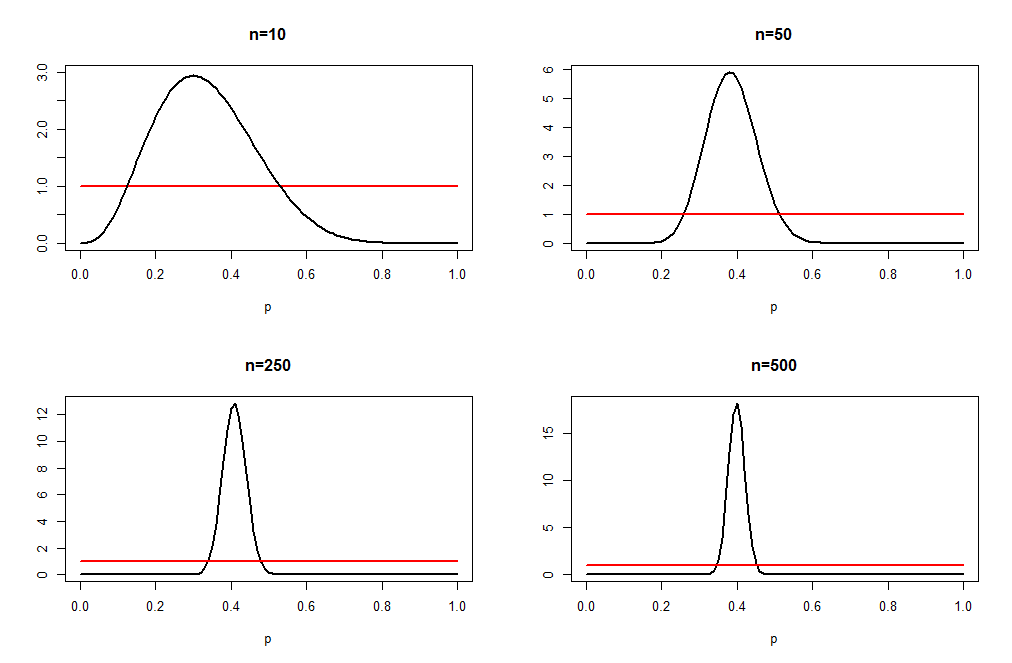
\includegraphics[width=\linewidth]{figures/post_priorunif.png}
\caption{\scriptsize Posterior densities for $\theta$,  for various sizes of the sample $n$ (prior distribution in red)}
  \end{figure}
 \end{frame}




%###########################################################
\begin{frame}\frametitle{Questions}

\begin{itemize}
 \item How to choose the prior ditribution?  
 \item  How to summarize the posterior distribution? How to do take decisions with the posterior distribution?
 \item Is it always easy to determine the posterior distribution? 
\end{itemize}

 
\end{frame}

%###########################################################

\subsection{About the prior distribution}
%###########################################################
\begin{frame}\frametitle{Choice of the prior distribution}
 \begin{columns}[t]
 \begin{column}{0.55\linewidth} 
  \begin{block}{}
\begin{itemize}
\item $\theta \in [0,1]$ :  $\theta \sim \mathcal{B}eta(a, b)$
\item $(a,b)$ are  hyperparameters
\item $ [\theta]  \propto  \theta^{a-1} (1-\theta)^{b-1} \ind_{[0,1]}(\theta)$ 
\item \vert How to chose $(a,b)$ ?  %$(a,b_k)$.  
\noir
\begin{itemize}
\item  If I don't know anything,  $a=b=1$ :  uniform distribution on $[0,1]$
 $$[\theta] \propto \ind_{[0,1]}(\theta)$$
 \item By tuning $a$ and $b$,  `` a priori'' give advantage to some values :  include  knowledge coming from previous studies or experts. 
 
% $$[\theta] \propto \prod_{k=1}^K \ind_{[0,1]}(p_k)$$
\end{itemize}
\end{itemize}
 \end{block} 
  \end{column}
  
\begin{column}{0.45\linewidth}
  \begin{block}{}
     \begin{figure}
 \centering
 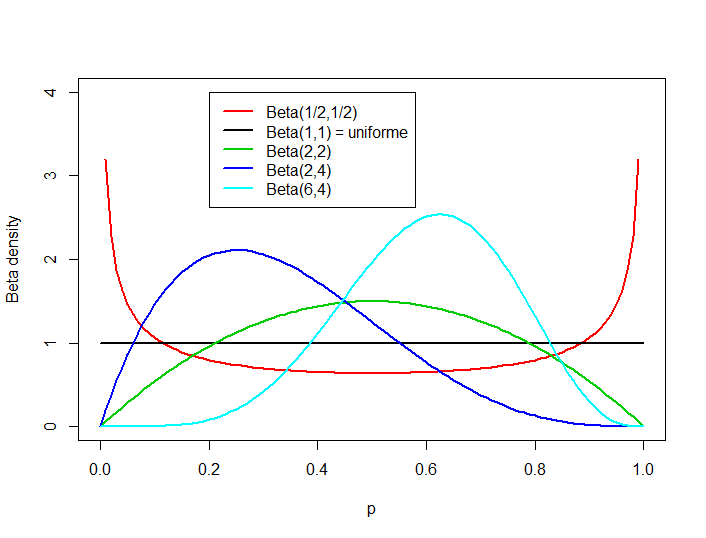
\includegraphics[width=\linewidth,height=\linewidth]{figures/plot_beta.png}
 \end{figure}
    \end{block}
  \end{column}
 \end{columns} 
\end{frame}


%###########################################################
\begin{frame}\frametitle{Posterior distribution}

\begin{eqnarray*}
 [\theta | \bY] &=& \frac{[\bY | \theta] [\theta]}{[\bY]} \propto [\bY | \theta] [\theta] \\
 &\propto&    \theta^{n_1} (1-\theta)^{n-n_1} \theta ^{a-1} (1-\theta)^{b-1}  \ind_{[0,1]}(\theta)\\ 
 &\propto&   \theta^{{\vert a+ n_1}-1} (1-\theta)^{{\vert b+n-n_1}-1}   \ind_{[0,1]}(\theta)\\
\end{eqnarray*}
We recognize 
$$\theta | \bY \sim \mathcal{B}eta(a + n_1, b+n-n_1)$$



\end{frame}

%###########################################################
\begin{frame}[fragile]\frametitle{Posterior distributions for various prior and $n$}
\centering
\begin{tabular}{cc}
   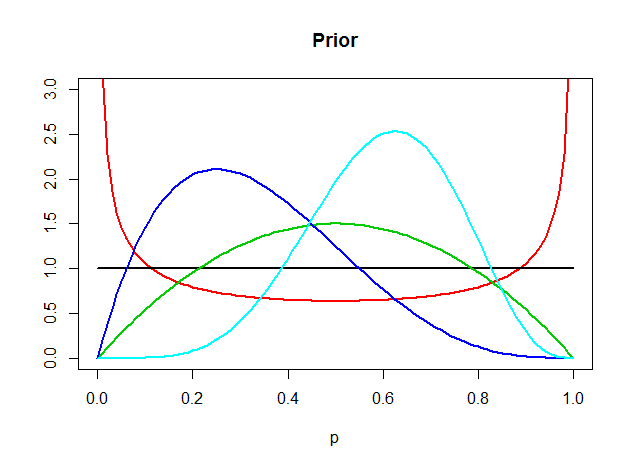
\includegraphics[width=0.4\linewidth]{figures/prior_beta.png} &
   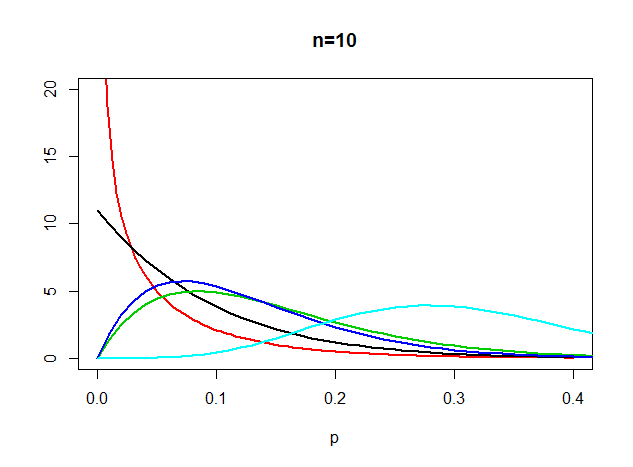
\includegraphics[width=0.4\linewidth]{figures/post_n=10.png} \\
      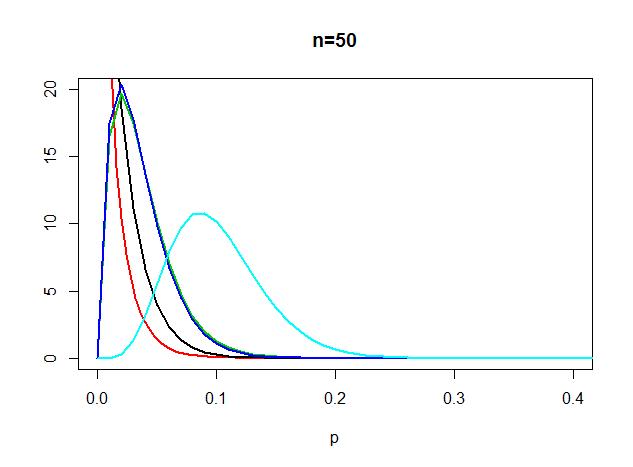
\includegraphics[width=0.4\linewidth]{figures/post_n=50.png}&
   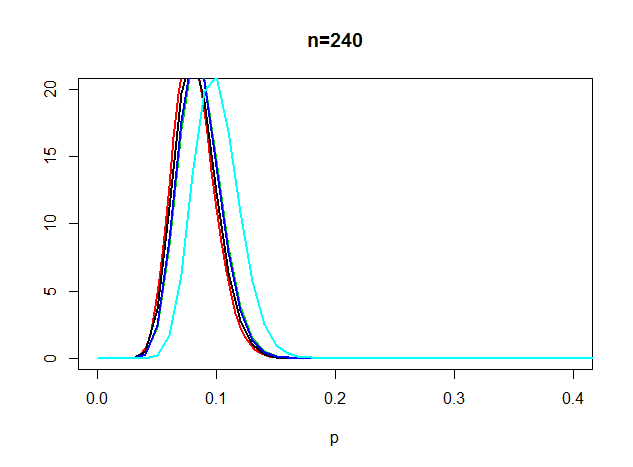
\includegraphics[width=0.4\linewidth]{figures/post_n=240.png} \\
\end{tabular}\\
\end{frame}

%###########################################################

%###########################################################
\begin{frame}\frametitle{Comments (1)}
\begin{itemize}
\item The  prior distribution on $\theta$ is updated  into a posterior distribution using the data
\item The posterior/prior distributions quantifies my incertitude on $\theta$
\item \vert Posterior\noir: compromise between the prior distribution and the data
\begin{eqnarray*}
p(\theta| \bY) &\propto& \pi(\theta) \ell(\by | \theta)\\
\log p(\theta | \by) &=& \log \pi(\theta)  +   \log \ell(\by | \theta) + C\\
\log p(\theta | \by) &=& \log \pi(\theta)  +  \sum_{i=1}^n \log \ell(y_i | \theta) + C
\end{eqnarray*}

\item The prior distribution has an influence on the posterior distribution if the number of observations $n$ is small

\item This influence vanishes if the number of observations increases 

\end{itemize}
\end{frame}
%###########################################################
\begin{frame}{Comments (2)}
 The prior distribution quantifies the prior (un)knowledge on $\theta$.
\begin{itemize} 
\item In case of complete prior incertitude : \vert non-informative prior \noir (Jeffreys: automatic construction. Improper prior) 
\item In case of external knowledge (previous experiments, experts) : \vert informative prior  
\end{itemize}
 
\end{frame}

%###########################################################
\begin{frame}\frametitle{Non informative prior}
If we do not know anything about $\theta$
  \begin{itemize}
\item Use an uniform prior as we did $\theta \sim \mathcal{U}_{[0,1]}$
\item The prior distribution can be improper  i.e $\int \pi(\theta) d \theta  = \infty$ provided the posterior distribution is a probability density
    \item Method to create an informative prior automatically:  \textbf{Jeffreys's prior}
    $$ \pi(\theta) \propto \sqrt{\det(I(\theta))}$$  where  $I(\theta)$ is the Fisher information (i.e. is big when the data contain a lot of information on the parameters )
    \begin{itemize}
    \item The prior gives more importance to values  such that  the data give a lot of informations about it:  minimizes the influence of the prior
    \end{itemize}
\end{itemize}
 
  
\end{frame}
%###########################################################

\subsection{Summary of the posterior distribution}

%###########################################################

\begin{frame}{Statistics for decisions}
 From my posterior distribution
 \begin{center}
 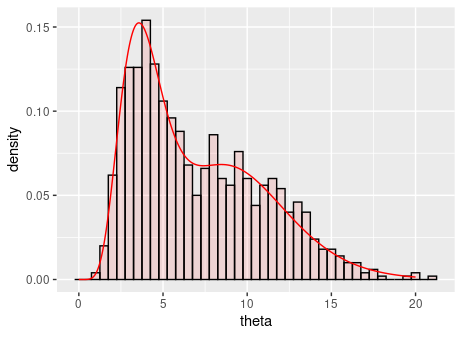
\includegraphics[width = 0.7 \textwidth]{figures/approx_post_MC.png}
 \end{center}
 
 \begin{multicols}{2}
    \begin{itemize}
      \item Parameter estimation
  \item Credible interval
  \item Hypothesis testing \footnote{\label{HOTS}Not evoked here}
  \item Model selection$^2$
    \end{itemize}
    \end{multicols}
   
 
\end{frame}


%###########################################################
\subsubsection{Estimation}
%###########################################################
 \begin{frame}\frametitle{Bayesian estimator}
 \begin{block}{Aim}
 Give an estimated value to $\theta$
 \end{block}
 
 Once we have the posterior distribution: 
 \begin{itemize}
 \item \vert Posterior expectation: \noir  $$E[\theta | \bY] = \int_{\theta} \theta [\theta | \bY]d\theta$$
 \item \vert Posterior median: \noir $$\P(\theta \leq q_{0.5} | \bY) = 0.5$$  
  \item \vert Maximum a posteriori MAP: 
    \noir $\arg\max_\theta \;  [\theta | \bY]$ 
  
 {\scriptsize  \begin{eqnarray*}
  \arg\max_\theta \;  [\theta | \bY] &=& \arg\max_{\theta} \; \log \ell(\bY | \theta)  + \log \pi(\theta) - \cancel{\vert \log P(\bY)}\\
%  &=&  \arg\max_{\theta} \; \log \ell(\bY | \theta)  + \log \pi(\theta)  \\
  &=& \arg\max_{\theta} \; \log \prod_{i=1}^n \P(Y_i | \theta)   + \log \pi(\theta)  \\
  &=& \arg\max_{\theta} \; \sum_{i=1}^n \log \P(Y_i | \theta)   + \log \pi(\theta)  
      \end{eqnarray*}}
 
  \end{itemize}
 
  \end{frame}
%###########################################################

  \begin{frame}\frametitle{Bayesian estimator in our example}
$$\theta \sim \mathcal{B}eta(a,b), \quad \quad \theta | \bY \sim \mathcal{B}eta(a + n_1, b+n-n_1)$$ 

  \begin{itemize}
 
\item\vert  Posterior expectation  \noir
$$ E[ \theta  | \bY] = \frac{a + n_1}{a + n_1+ b+n-n_1} = \frac{a + n_1}{a+b+n}$$
\item \vert MAP \noir
 $$\arg\max_\theta [\theta | \bY] =  \frac{a + n_1 - 1}{a + n_1+ b+n-n_1-2} = \frac{a + n_1-1}{a+b+n-2}$$
 \item \vert Posterior median \noir : no explicit expression 
 $$\approx \frac{a + n_1 - \frac{1}{3}}{a + n_1 +  b+n-n_1 - \frac{2}{3}} =  \frac{a + n_1 - \frac{1}{3}}{a +   b+n - \frac{2}{3}}$$
\end{itemize}
 
  \end{frame}
%###########################################################
      
   
\subsubsection{Credible interval}
  
%----------------------------------------------------------------------------- 
\begin{frame}[allowframebreaks]\frametitle{Credible interval }

  \begin{block}{Aim}
 Finding the shortest (if possible)  interval such that $$\P(\theta \in [a,b] | \bY) = 1- \alpha$$
 \end{block}
 
 Several ways to define it : 
 
\begin{block}{Highest posterior density interval  (HPD)}
It is the narrowest interval, which for a unimodal distribution will involve choosing those values of highest probability density including the mode.
 $ \mathcal{C} = \{\theta;\pi(\theta  | \bY)  \geq k\} $ where $k$ is the largest number such that $\int_{\theta; \pi(\theta  | \bY) \geq k} \pi(\theta | \bY) d\theta=1- \alpha$ 
\end{block}

\begin{figure}
\centering 
 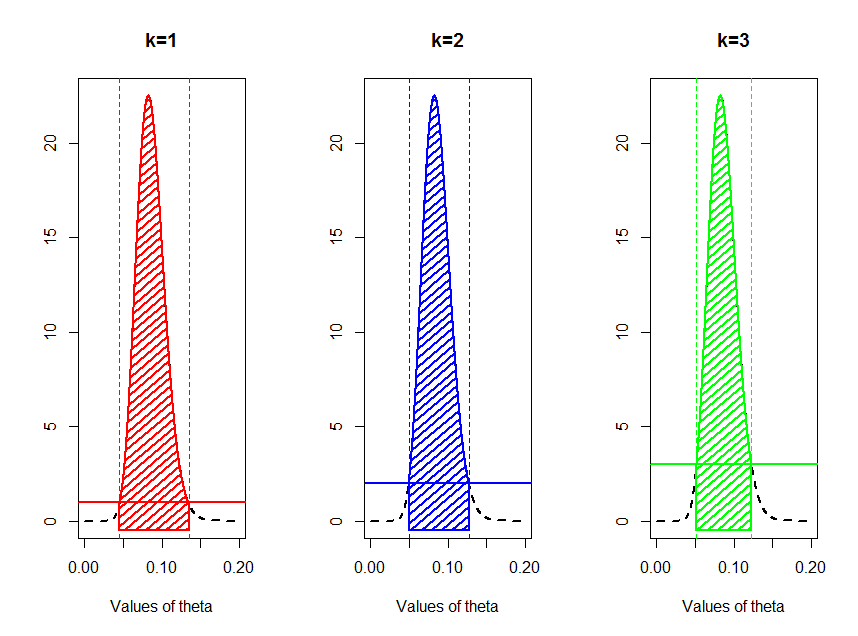
\includegraphics[width=\linewidth]{figures/HPD.png}
 \end{figure}
\end{frame}

\begin{frame}\frametitle{Highest posterior density region }

 \begin{figure}
\centering 
 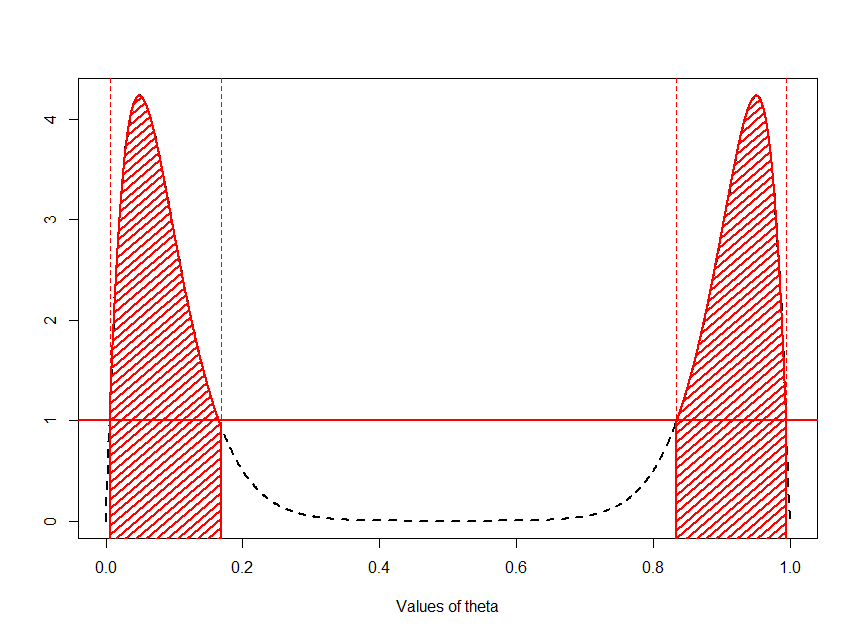
\includegraphics[width=0.6\linewidth]{figures/HPD_bimod.png}
 \end{figure}

\begin{itemize}
\item Be careful : if the posterior density is multi-modal, one can get the union of 2 intervals. 
\item Difficult to get in practice because we have to invert the density function
\end{itemize}

\end{frame}
%###########################################################
\begin{frame}

\begin{block}{Equal-tailed interval} 
Choosing the interval where the probability of being below the interval is as likely as being above it. This interval will include the median. 
\end{block}

\begin{figure}
\centering 
 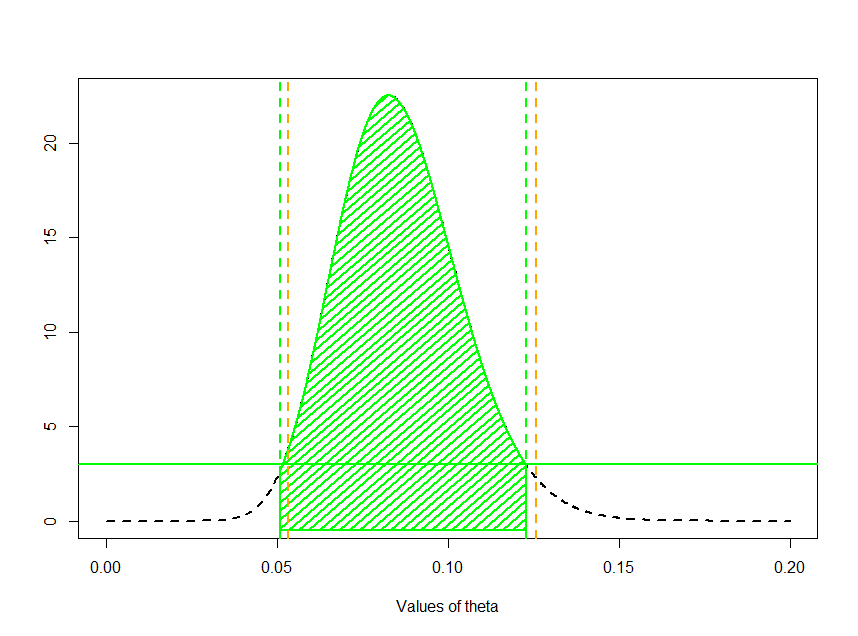
\includegraphics[width=0.8\linewidth]{figures/Equi_tailes.png}
 \end{figure}
 
  \hyperlink{BF}{\beamergotobutton{Hypothesis testing and model selection}}
 
\end{frame}
%###########################################################

%###########################################################

\begin{frame}{Take home messages}
\label{TakeHOME}
 

\begin{block}{}
\begin{itemize}
\item Bayesian statistics are only related to statistical inference (estimation, hypothesis testing...) 
\item A statistical model  is not Bayesian per se (except in neurosciences where some of them consider that the brain is ITSELF Bayesian)
\item Bayesian inference  is based on a prior distribution on the unknown quantities (parameters, models...) 
\item The prior distribution quantifies the knowledge on the unknown quantities  BEFORE the experiment. We can know nothing (non-informative prior) or  something from previous studies, from experts (informative prior). 
\item The sensibility to the prior has to be analysed to be aware of this influence
\end{itemize}
\end{block}
\end{frame}

%###########################################################

\begin{frame}{Focus on this class}
\begin{itemize}
\item Bayesian decision is a large topic. 
\item Focus of this course on the methods to obtain the posterior distribution.
\end{itemize}
 \end{frame}

%###########################################################
\subsection{Determining the posterior distribution}

\subsubsection{Conjugate case}

\begin{frame}{Conjugate prior : easy case}

In our example : beta prior \color{blue}$\rightarrow$ \color{black} beta posterior
\begin{itemize}
\item We talk about conjugate prior when the prior and the posterior distributions are in the same family 
\item \vert Examples \color{black}
\end{itemize}
$$
\begin{array}{|c|c|c|c|} 
\hline
\left[y| \theta\right]  & [\theta]  & [ \theta|y ]& \mathbb{E}[\theta|y]\\
 \hline 
 \mathcal{N}(\theta,\sigma^2)& \mathcal{N}(\mu,\tau^2)& \omega^2 = [\frac{1}{\sigma^2} + \frac{1}{\tau^2}]^{-1} & \omega^{2}(\frac{y}{\sigma^2} + \frac{\mu}{\tau^2})\\
 & &   \mathcal{N}(\omega^{2}(\frac{y}{\sigma^2} + \frac{\mu}{\tau^2}),\omega^2 )&\\
% %& & &\\
 \Gamma(n,\theta)  & \Gamma(\alpha, \beta) &   \Gamma(\alpha+y, \beta+n)& \frac{\alpha+x}{\beta+n}\\ 
% %%& & &\\
 \mathcal{B}in(n, \theta)&  \mathcal{B}(\alpha,\beta) & \mathcal{B}(\alpha + y, \beta + n - y )&  \frac{\alpha + y}{\alpha + n + \beta}\\
 \mathcal{P}(\theta) &  \Gamma(\alpha, \beta)&  \Gamma(\alpha + y, \beta + 1)&  \frac{\alpha + x}{\beta + 1}\\
 \hline
\end{array}$$
\color{dgreen}{ \footnotesize \href{https://en.wikipedia.org/wiki/Conjugate_prior}{See  Wikipedia for instance}}\color{black}

\end{frame}


%%%%%%%%%%%%%%%%%%%%%%%%%%%%%%%%%%%%%%%%%%%%%%%
\begin{frame}{To go further}

\begin{itemize}
\item For the exponential family of distributions, we have  a conjuguate prior \color{blue}$\rightarrow$ \color{black} very rare in practice
\item Note that the Gaussian regression model is congugate: 
\begin{eqnarray*}
 \bY &\sim& \mathcal{N}(X\beta,\sigma^2 \mathbb{I})\\
 \beta  | \sigma &\sim& \mathcal{N}(\beta_0,\sigma^2\Omega)
\end{eqnarray*}
Then, 


\item  For any more complex  model, (such as Latent Variable models)  the posterior distribution is not explicit
% \item People resort to 
% \begin{itemize}
%  \item Sampling methods
%  \item Approximation methods
% \end{itemize}
\end{itemize}
\end{frame}

%%%%%%%%%%%%%%%%%%%%%%%%%%%%%%%%%%%%%%%%%%%%%%%
\begin{frame}{Illustration on the mixture model}

{\footnotesize \vert In a few words\noir:  My data $y_i$ are issued from to populations, each population having its own mean. I do not know to which population each observation belongs. 
}

\begin{itemize}
 \item \vert Model \noir $Z_i \in \{1,2\}$
 \begin{eqnarray*}
 P(Z_i = 1) &=& \pi_1\\
 Y_i  | Z_i = k  &\sim&  \mathcal{N}(\mu_k,1)
 \end{eqnarray*}
\item \vert Parameters: \noir $\theta = (\pi_1,\mu_1,\mu_2)$
\item \vert Likelihood: \noir
 
\begin{eqnarray*}
[\bY | \theta] = \prod_{i=1}^n \left[\pi_1 \frac{1}{\sqrt{2\pi}}e^{-\frac{1}{2}(y_i-\mu_1)^2} + (1-\pi_1)\frac{1}{\sqrt{2\pi}}e^{-\frac{1}{2}(y_i-\mu_2)^2} \right]
\end{eqnarray*}

 
\item \vert Prior distribution: \noir
 $$\pi_1 \sim \mathcal{U}_{[0,1]}, \quad \mu_k \sim \mathcal{N}(0,\omega^2), \quad k=1,2$$
 \end{itemize}
\end{frame}

 
%----------------------------------------------------------------------------- 
\begin{frame}{Mixture distribution : posterior}

\begin{eqnarray*}
[\theta | \bY] &\propto&   [\bY | \theta] [\theta]\\
&\propto & \prod_{i=1}^n \left[\pi_1 \frac{1}{\sqrt{2\pi}}e^{-\frac{1}{2}(y_i-\mu_1)^2} + (1-\pi_1)\frac{1}{\sqrt{2\pi}}e^{-\frac{1}{2}(y_i-\mu_2)^2} \right]   \ind_{[0,1]}(\pi_1)  \\
&&  \frac{1}{\omega \sqrt{2\pi}}e^{-\frac{1}{2 \omega^2} \mu_1 ^2} \frac{1}{\omega \sqrt{2\pi}}e^{-\frac{1}{2 \omega^2} \mu_2 ^2}
\end{eqnarray*}


\begin{itemize}
\item  Non conjuguate model, posterior distribution not explicit.
\item  How to evalute, for instance the \vert posteriori mean:\noir $\int \theta [\theta | \bY] d\theta$?  
\end{itemize}
\end{frame}

 

\subsubsection{Outside the conjugate case}

%%%%%%%%%%%%%%%%%%%%%%%%%%%%%%%%%%%%%%%%%%%%%%%
\begin{frame}{How to determine a complex posterior distribution?}


\begin{itemize}
 \item Resort to algorithms to approximate the posterior distribution.
 \item 2 approaches
\begin{itemize}
 \item \vert Sampling methods\noir: supply realizations of the posterior distribution $\theta^{(1)}$, $\dots$, $\theta^{(m)}$, $\dots$, $\theta^{(M)}$.
 \item \vert Deterministic methods\noir: approximate  the density $p(\theta | \bY)$ in a given family of distribution. 
\end{itemize}
\end{itemize}
\end{frame}

%%%%%%%%%%%%%%%%%%%%%%%%%%%%%%%%%%%%%%%%%%%%%%%
\begin{frame}{Sampling methods}

\begin{block}{}
If we can simulate $\theta^{(m)} \sim_{i.i.d.} P(\theta | \by)$ for $m=1,\dots, M$, then 
$\frac{1}{M} \sum_{m=1}^M \delta_{\theta^{(m)}}(\cdot) \approx p(\cdot | \by)  $
(Glivenko-Cantelli theorem)
\end{block}

\centering
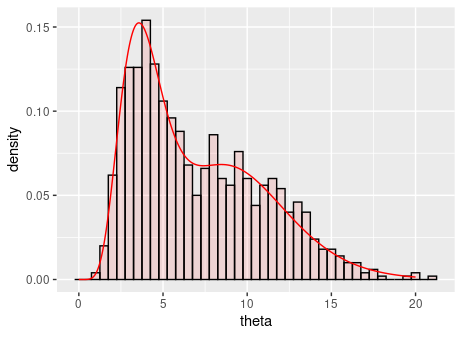
\includegraphics[width = 0.5\textwidth]{figures/approx_post_MC.png}

\begin{itemize}
\item \emph{Law of large numbers} : $\frac{1}{M} \sum_{m=1}^M  \theta^{(m)}$ approximates$^*$  $E[\theta | \by]$
\end{itemize}
\end{frame}

%%%%%%%%%%%%%%%%%%%%%%%%%%%%%%%%%%%%%%%%%%%%%%%

\begin{frame}{Monte Carlo Markov Chains methods }

Gibbs Sampler, Metropolis-Hastings algorithm...
\begin{itemize}
\item \vert\emph{Main idea}\color{black}: design a Markov Chain such that its stationary distribution is the posterior distribution
\item Generic methods
\item Supplies asymptotically realizations of the posterior distribution $\theta^{(1)}$, $\dots$, $\theta^{(m)}$, $\dots$, $\theta^{(M)}$
\item Made the success of the Bayesian inference
\end{itemize}
\end{frame}

%%%%%%%%%%%%%%%%%%%%%%%%%%%%%%%%%%%%%%%%%%%%%%%

\begin{frame}{Importance samplers}
\begin{itemize}
 \item Simulate ``particles''  $\theta^{(1)}, \dots, \theta^{(m)}, \dots, \theta^{(M)}$ with a ``simple'' distribution
  \item Give weights to the particles to correct the discrepancy between the distribution used to simulate and the posterior distribution
 \end{itemize}
\end{frame}
%%%%%%%%%%%%%%%%%%%%%%%%%%%%%%%%%%%%%%%%%%%%%%%
\begin{frame}{Deterministic approximation}

Variational Bayes for instance
 \begin{itemize}
 \item Approximate the density $p(\theta | \by)$ in a given family of distribution 
 \item Minimizes a divergence with the true posterior density.  
  \item Optimization
\end{itemize}
 

 
\end{frame}





 

%!TEX root = donnet_bayesianLVM_main.tex

%====================================================================
\section[MCMC]{Sampling the posterior distribution by MCMC algorithms} 
%====================================================================
 \subsection{Some more complex models}
%====================================================================
\begin{frame}{Example 1 : non linear model}
%====================================================================
Assume that we want to explain  the presence of hallucination by the patient age and the moment the disease began 
  \begin{itemize}
 \item For any individual $i$, $Y_i  =1$ if we observe hallucinations
 \item Co-variables: $X_ i = (A_i, D_i)$ are the age, and the moment the disease appeared in patient $i$
 \item \vert Generalized linear model :  Probit regression  \noir 
 
\begin{eqnarray*}
Y_i &\sim& \mathcal{B}ern(p_i) \\
p_i&=& \Phi(\theta_0 + \theta_1 A_i + \theta_2 D_i) = \Phi(^tX_i \btheta)
\end{eqnarray*} 
where  $\btheta = ^t(\theta_1,\theta_2,\theta_3)$ et  $\Phi : \R \mapsto [0,1]$ is the cumulative probability function of a $\mathcal{N}(0,1)$
  \end{itemize}
 
 \end{frame}
%====================================================================
\begin{frame}{Likelihood, prior, posterior}
%====================================================================
  \begin{itemize}
   \item $\btheta=(\theta_0,\theta_1,\theta_2)$
 \item \vert  Likelihood \noir
 
 \begin{eqnarray*}
 [\bY | \btheta] &=& \prod_{i=1}^n \Phi(\theta_0 + \theta_1 A_i + \theta_2 D_i)^{Y_i} (1- \Phi(\theta_0 + \theta_1 A_i + \theta_2 D_i))^{1-Y_i} 
 \end{eqnarray*}
 \item \vert Prior distribution on  $\btheta \in \R^3$\noir
 $$\pi(\btheta)  \sim \mathcal{N}(0_{\R^3}, \omega \mathbb{I}_3), \quad \mbox{ or } \quad \pi(\btheta) \propto 1$$
 
 
  \item \vert Posterior distribution on $\btheta$\noir
\begin{eqnarray*} 
[\btheta | \bY] &\propto&  [\bY | \theta] [\btheta] \\
 &\propto& \prod_{i=1}^n \Phi(\theta_0 + \theta_1 A_i + \theta_2 D_i)^{Y_i} (1- \Phi(\theta_0 + \theta_1 A_i + \theta_2 D_i))^{1-Y_i}
\end{eqnarray*}
 \centering
 \vert Non conjugated case, no  explicit expression of the posterior $[\btheta | \bY]$
 \end{itemize}
 \end{frame}
 
%====================================================================
\begin{frame}{Example 2: nlme}
%====================================================================
 
 Orange dataset
\begin{itemize}
 \item $y_{ij}$ : circumference of orange tree $i$ at age $t_{ij}$
 \item $i = 1,\dots,5$, $n_{i}=5$.
\end{itemize}

\centering
 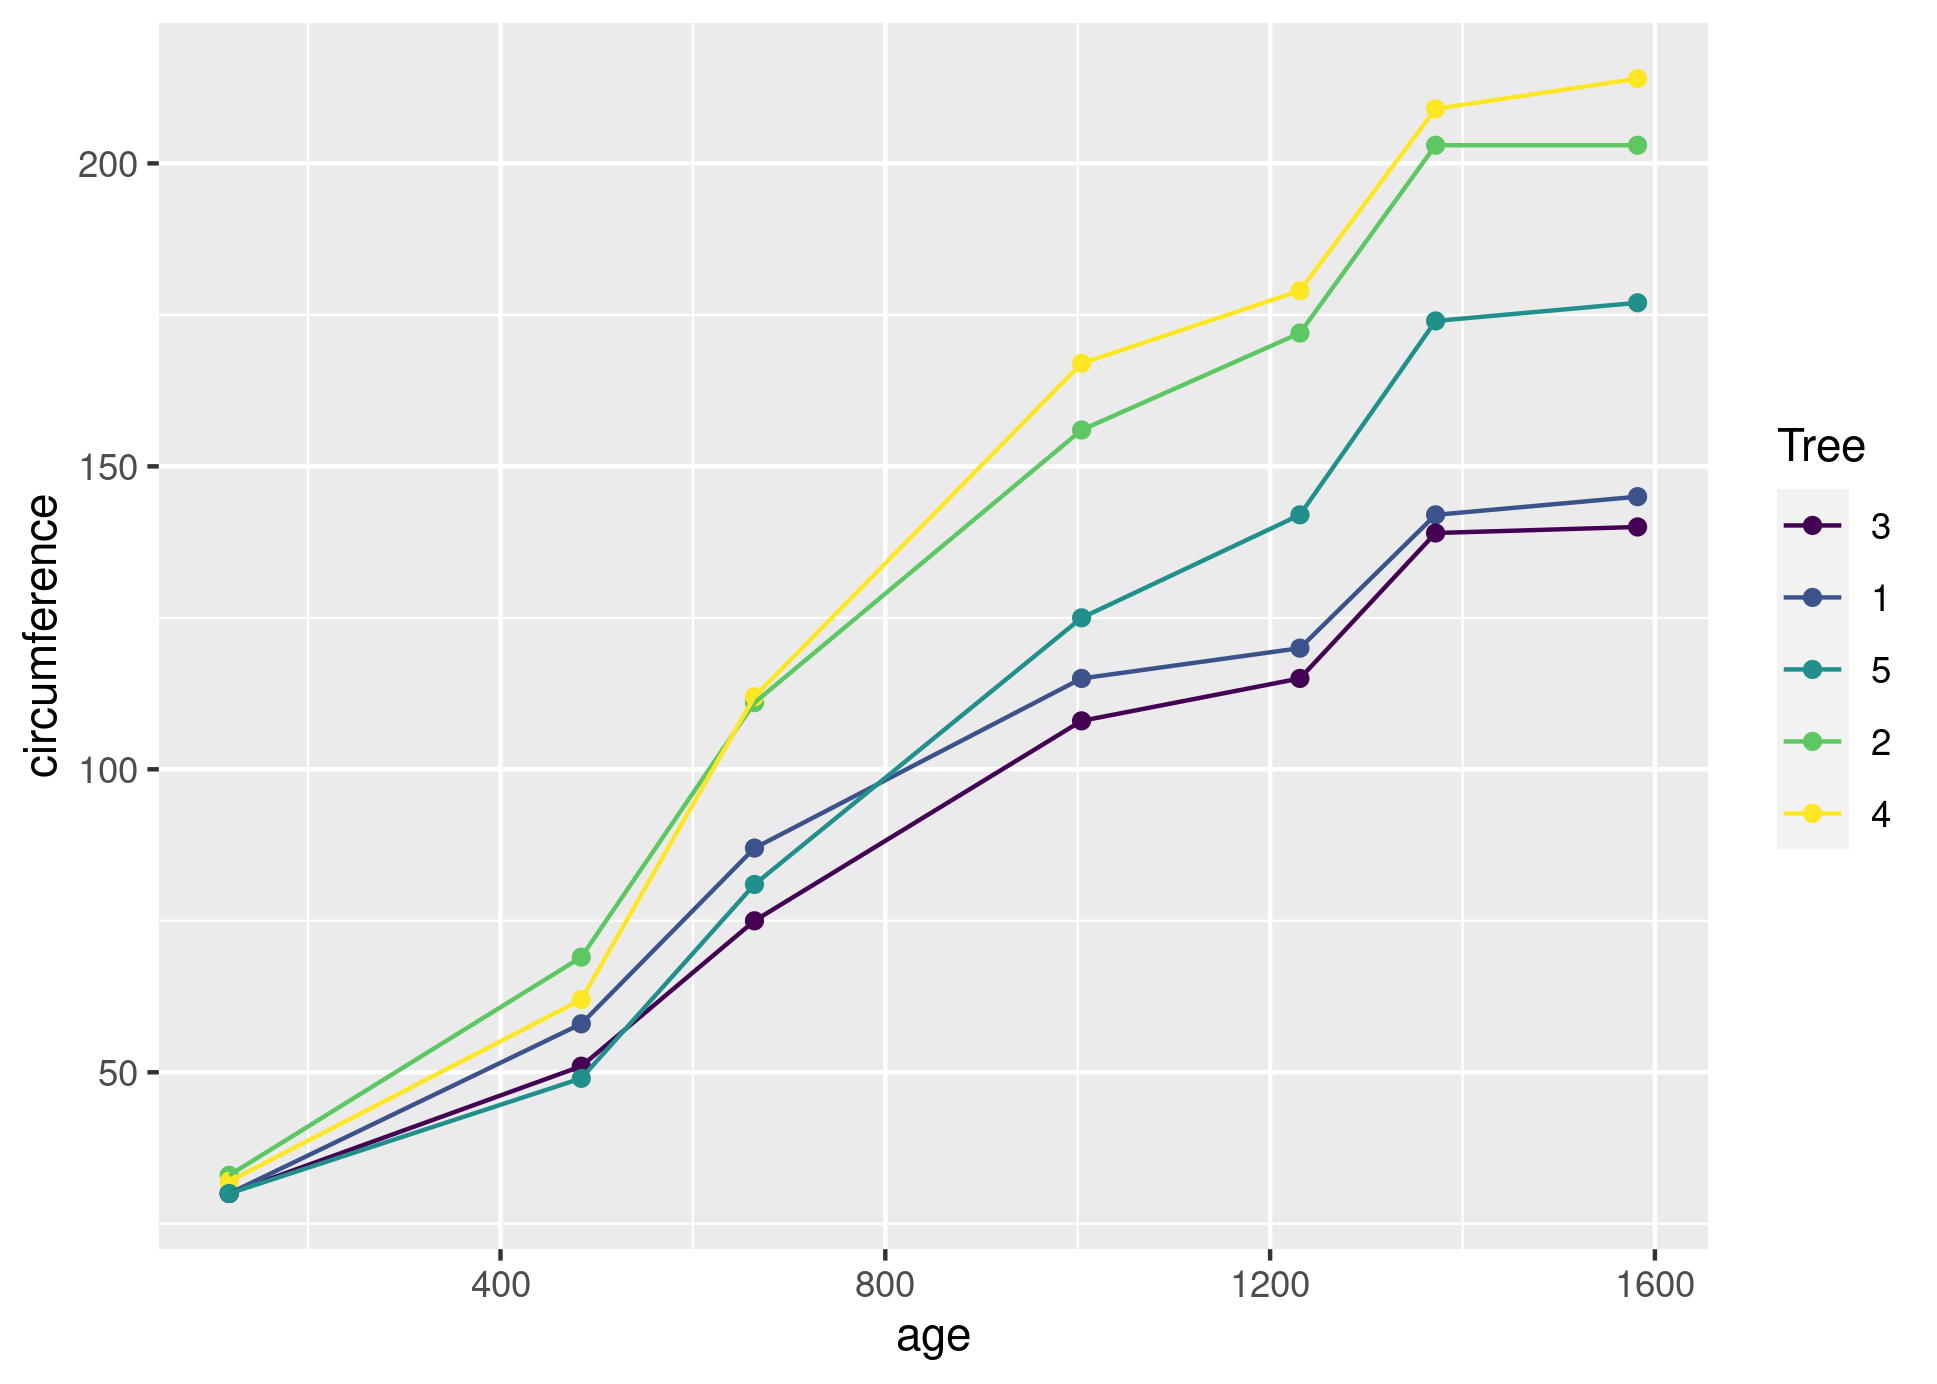
\includegraphics[width = 0.7 \linewidth]{figures/OrangeData.png}
 \end{frame}

 
%====================================================================
 \begin{frame}{Example 2: nlme}
%====================================================================
 
  \begin{columns}[t]
 \begin{column}{0.50\linewidth} 
  \begin{block}{}
   \begin{itemize}
  \item Logistic relation between $y$ and $t$
  $$ f(t;\phi) = \frac{a}{1+e^{-\frac{t-b}{c}}}$$
  \item  Gaussian noise
  \item Individual effect of each tree
 \end{itemize}
   
  \end{block}
\end{column}

  \begin{column}{0.50\linewidth} 
  \begin{block}{Latent variable model}
 
\begin{eqnarray*}
Y_{ij} &=& \frac{A + a_{i}}{1+e^{-\frac{t-(B+b_i)}{C+c_i}}} + \varepsilon_{ij}\\
\varepsilon_{ij} &\sim& \mathcal{N}(0,\sigma^2)\\
a_i &\sim_{i.i.d}& \mathcal{N}(0, \omega^2_a)\\
b_i &\sim_{i.i.d}& \mathcal{N}(0, \omega^2_b)\\
c_i &\sim_{i.i.d}& \mathcal{N}(0, \omega^2_c)
\end{eqnarray*}
   \end{block}
   \vspace{1em}
   
\end{column}
\end{columns}
 
 
 \begin{itemize}
  \item {\vert Latent variables} : $\ba  =  (a_1,\dots,a_5)$,$\bb = (b_1,\dots,b_5)$, $\bc = (c_1,\dots,c_5)$
  \item {\vert Parameters} :  $\theta = (A,B,C,\omega^2_a,\omega^2_b,\omega^2_c,\sigma^2)$
 \end{itemize}

 \end{frame}

%====================================================================
 \begin{frame}{Example 2: likelihood}
%====================================================================

{\small 
\begin{eqnarray*}
 p(\by | \ba,\bb,\bc;\theta) &=& \prod_{i=1}^5 \prod_{j=1}^{n_{i}} \frac{1}{2\pi \sqrt{\sigma^2}} \exp\left[-\frac{1}{2\sigma^2}\left(y_{ij}- f(t_{ij};A+a_i,B+b_i,C+c_i)\right)^2\right]\\
 p(\ba;\theta)  &=& \prod_{i=1}^5 \frac{1}{2\pi \sqrt{\omega_a^2}}  \exp\left[-\frac{1}{2\omega_a^2} a_i^2\right]\\
 p(\bb;\theta)  &=& \prod_{i=1}^5 \frac{1}{2\pi \sqrt{\omega_b^2}}  \exp\left[-\frac{1}{2\omega_b^2} b_i ^2\right]\\
 p(\bc;\theta)  &=& \prod_{i=1}^5 \frac{1}{2\pi \sqrt{\omega_c^2}}  \exp\left[-\frac{1}{2\omega_b^2} c_i^2\right]\\
  \ell(\by;\theta) &=& \int_{\ba,\bb,\bc} p(\by|\ba,\bb,\bc;\theta)p(\ba;\theta) p(\bb;\theta) p(\bc;\theta) d\ba\;  d\bb \;  d\bc 
\end{eqnarray*}}

\centering Not an explicit expression \color{dgreen} $\Rightarrow$ \color{black} Impossible to get an expression of the posterior distribution
 
 \end{frame}


%====================================================================
\begin{frame}{A few words on MCMC}
%====================================================================
 
\begin{itemize}
 \item Enabled the development of Bayesian inference in the  90's
 \item Stochastic algorithms
\end{itemize}

\begin{block}{Principle}
 \begin{itemize}
 \item  \vert Principle: \noir generates a Markov Chain  $\btheta^{(m)}$ whose ergodic distribution  (asymptotic, after a large number of iterations) is the distribution of interest  $[\btheta |\bY]$
 \item \vert What it will produce : \noir a sample  ($\btheta^{(1)} ,\dots, \btheta^{(M)}$) from the distribution $[\btheta | \bY]$
 \item \vert What will I do with it?  \noir  this sample supplies an approximation of the posterior distribution  (so : histograms, moments, quantiles...) 
 $$ \widehat{E[\btheta | \bY]} = \frac{1}{M}\sum_{m=1}^M \btheta^{(m)}$$
\end{itemize}

\end{block}


\end{frame}
 

 %====================================================================
 \subsection{Metropolis Hastings}
%====================================================================
\begin{frame}[allowframebreaks]{Metropolis-Hastings algorithm}
%====================================================================
\begin{itemize}
 \item  Belongs to the family of  {\vert M}onte {\vert C}arlo {\vert M}arkov {\vert C}hains
 \item \vert Idea\noir: explore the posterior distribution  with a random walk using a proposal distribution to move.
 \end{itemize}
 
 \begin{tabular}{ccc}
  
  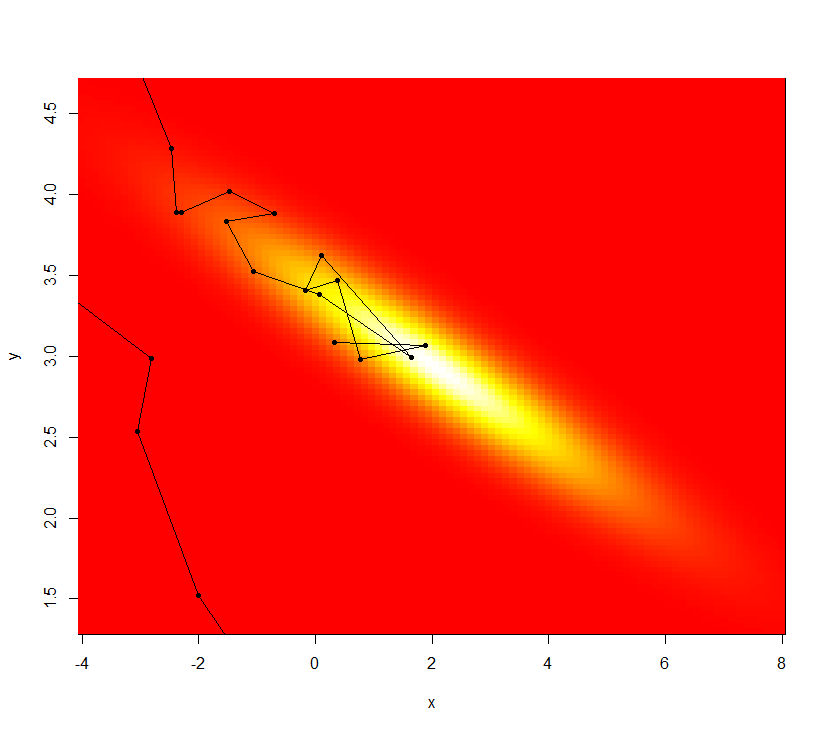
\includegraphics[width=0.3\textwidth]{figures/MCMC_chain_debut.png}&
  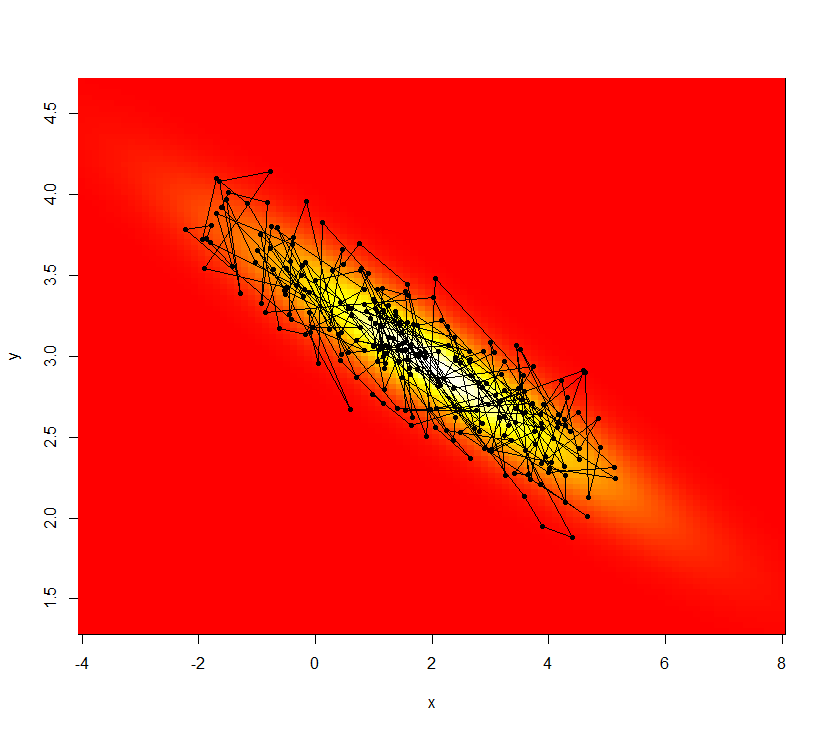
\includegraphics[width=0.3\textwidth]{figures/MCMC_chain_milieu.png}&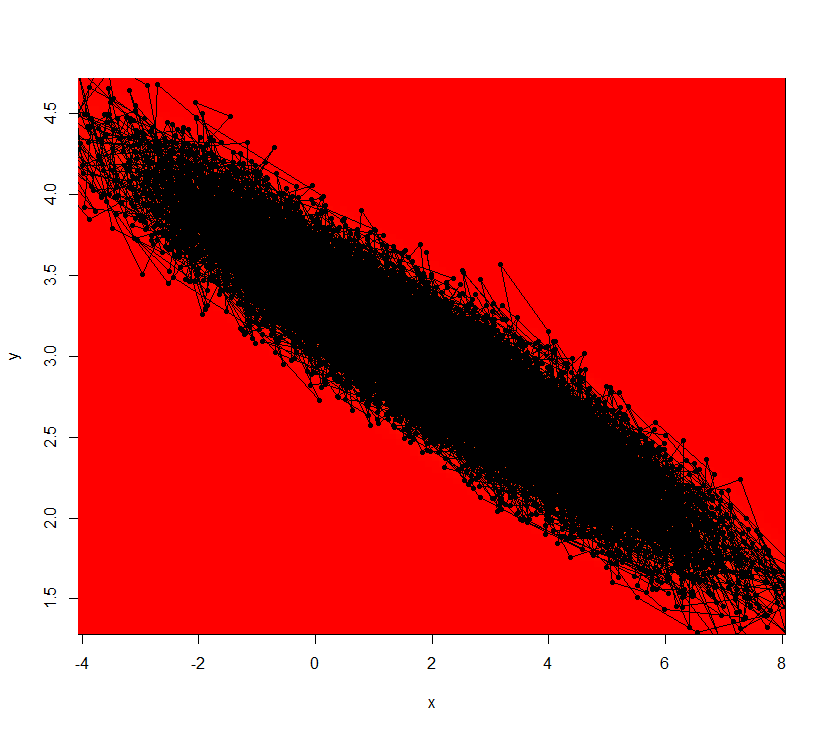
\includegraphics[width=0.3\textwidth]{figures/MCMC_plot_50000.png}
% 
 \end{tabular}

\begin{itemize}
 \item Let's chose an instrumental distribution  $q(\btheta' | \btheta)$  which can be easily simulated.  
  \end{itemize}
 
\begin{block}{A iteration $0$}
   Initialize  $\theta^{(0)}$ arbitrarily chosen  
\end{block}
     
     
 \begin{block}{At iteration  $m$}
 \begin{enumerate}
 \item Propose a candidate $\btheta^{c} \sim q(\btheta^{c} | \btheta^{(m-1)})$
 \item Calculate an acceptance probability :  
 $$ \rho(\btheta^c | \btheta^{(m-1)} )= \min\left\{1, \frac{[\btheta^{c} | \bY] }{[\btheta^{(m-1)}| \bY]} \frac{q(\btheta^{(m-1)} | \btheta^{c})}{q(\btheta^{c} | \btheta^{(m-1)})}\right\} $$
 \item  Accept the candidate with probability  $\rho(\btheta^c | \btheta^{(m-1)} )$, i.e. 
 $$u \sim \mathcal{U}_{[0,1]} \quad \mbox{et} \quad 
  \btheta^{(m)} = \left\{ \begin{array}{cl} \btheta^c & \mbox{ si } u<  \rho(\btheta^c | \btheta^{(m-1)} )\\
  \btheta^{(m-1)}  & \mbox{ sinon} 
  \end{array}
  \right.
  $$ 
\end{enumerate}
\end{block}
\end{frame}

  %====================================================================
 \begin{frame}{Why can I apply it?  }
 %====================================================================
  $$ \rho(\btheta^c | \btheta^{(m-1)} )= \min\left\{1, \frac{\vert [\btheta^{c} | \bY] }{\vert [\btheta^{(m-1)}| \bY]} \frac{q(\btheta^{(m-1)} | \btheta^{c})}{q(\btheta^{c} | \btheta^{(m-1)})}\right\} $$
  

\begin{eqnarray*}
 \frac{\vert [\btheta^{c} | \bY] }{\vert [\btheta^{(m-1)}| \bY]} &=& \frac{[\bY| \btheta^{c} ][\btheta^{c}]/\cancel{\vert [\bY]} }{[\bY| \btheta^{(m-1)} ][\btheta^{(m-1)}]/\cancel{\vert [\bY]}}\\
 &=& \frac{[\bY| \btheta^{c} ][\btheta^{c}]  }{[\bY| \btheta^{(m-1)} ][\btheta^{(m-1)}]}
 \end{eqnarray*}

 \begin{itemize}
  \item Easy to compute provided I know how to evaluate the likelihood
  \item Metropolis-Hastings :  universal (can be used in a large number of cases $=$ models)
   \end{itemize}
\vert 
\end{frame}

%====================================================================
 \begin{frame}{Random walk : particular choice of $q$}
 %====================================================================
  
 \vert Required qualities on $q$:  \noir  easy to propose a candidate: easy to  simulate, explicit probability density, with a support larger than the one of the distribution of interest 
 
 
 \begin{itemize}
 \item 
  $$ \theta^{c}  = \theta^{(m-1)} + \xi, \quad \quad \xi\sim \mathcal{N}_d(0_d, \tau^2 \mathbb{I}_d)$$
 %\item  where here  $\hat{\Sigma}$ is the asymptotic covariance matrix of the MLE  $\hat \btheta$
  \item In this case, symmetric kernel: $q(\btheta^{c} | \btheta^{(m-1)}) = q(\btheta^{(m-1)}| \btheta^{c} )$. 
  \end{itemize}
% \item \vert Example 2: independant kernel   \noir 
% $$q(\btheta^{c} | \btheta^{(m-1)})  =[\btheta^{c} ]$$  
 
 \begin{block}{Warning}
The choice of the transition kernel  $q(\cdot | \cdot)$ strongly influences the theoretical and practical convergence properties.  
\end{block}
\end{frame}
 
 
%====================================================================
\begin{frame}{Visualisation of the principle}
%====================================================================

We have a look at the wonderful interactive viewer by Chi Feng. 
\href{https://chi-feng.github.io/mcmc-demo/app.html?algorithm=RandomWalkMH&target=banana}{\beamergotobutton{chi-feng interactive MCMC}}


\end{frame}


%====================================================================
\begin{frame}{MH : convergence} 
%====================================================================
 \begin{itemize}
  \item By construction : $[\theta | \bY]$ is stationary 
  \item Explicit transition kernel
   $K(\theta' | \theta)$
  \item Prove that for any Borel set $A$
  $$ \int_{\theta' \in A} \int_\theta K(\theta'|\theta) p(\theta  | \by)  d\theta  d \theta' = \int_{\theta' \in A}p(\theta' | \by) d \theta'$$
 \end{itemize}
\end{frame}
%====================================================================
\begin{frame}{MH : kernel transition $K(\theta' | \theta)$} 
%====================================================================
Kernel transition such that
\begin{eqnarray*}
  \btheta^c &\sim& q(\btheta^c | \btheta)\\
  Z &\sim& \mathcal{B}ern(\alpha(\theta^c | \theta))\\
 \btheta' &=& Z \btheta^c    + (1-Z)  \btheta
 \end{eqnarray*}
 
Let's prove that  
  \begin{block}{}
$$K(\theta' | \theta) =   \alpha(\theta' | \theta) q(\theta'|\theta)  + r(\theta) \delta_{\theta}(\theta')$$
where
$$r(\theta) = \int_{\theta^c} (1-\alpha(\theta^c | \theta)) q (\theta^c | \theta) d \theta^c$$
\end{block}

 
\end{frame}
%====================================================================
 \begin{frame}{Kernel transition. Proof} 
%====================================================================
 For any measurable function $\phi$ we need $\mathbb{E}[\phi(\theta') | \theta]  = \int \phi(\theta')K(\theta' | \theta) d\theta'$

{\small 
\begin{eqnarray*}
 \mathbb{E}[\phi(\theta') | \theta]  &=&    \mathbb{E}_{\theta^c,Z}[\phi(Z \btheta^c    + (1-Z)  \btheta)] \pause \\ 
 &=&    \mathbb{E}_{\theta^c,Z}[Z \phi(\btheta^c)    + (1-Z)  \phi(\btheta)] \pause\\
&=& \int_{\theta^c} \left[\phi(\btheta^c)\mathbb{P}(Z = 1 | \theta) +  \phi(\btheta) \mathbb{P}(Z = 0 | \theta)\right] q(\btheta^c | \btheta) d \theta^c \pause \\ 
 &=&  \int_{\theta^c}  \phi(\btheta^c)\alpha(\theta^c | \theta) q(\btheta^c | \btheta) d \theta^c  + \phi(\theta)\underbrace{ \int_{\theta^c} (1-\alpha(\theta^c | \theta)) q (\theta^c | \theta) d \theta^c}_{r(\theta)} \pause\\
 &=& \int_{\theta'} \phi(\theta') \alpha(\theta' | \theta) q(\theta'|\theta)d\theta'  + r(\theta) \phi(\theta) \pause \\
&=&  \int_{\theta'} \phi(\theta')    \alpha(\theta' | \theta) q(\theta'|\theta)  + r(\theta) \int_{\theta'} \phi(\theta') \delta_{\theta}(\theta')  d\theta' \pause \\
&=&  \int_{\theta'} \phi(\theta')  \left\{ \alpha(\theta' | \theta) q(\theta'|\theta)  + r(\theta) \delta_{\theta}(\theta')\right\} d\theta'   
\end{eqnarray*}
 }



\end{frame}

%==================================================================== 
\begin{frame}{MH : stationarity}
%====================================================================


We have to prove that  for any subset $A$, 

$$ \int_{\theta' \in A}\int_{\theta} K(\theta' | \theta) p(\theta|y) d\theta d\theta'= \int_{\theta' \in A} p(\theta' | y) d\theta'$$
 
 
 
\end{frame}
 
 

%==================================================================== 
\begin{frame}{Proof of stationarity I}
%====================================================================


\begin{eqnarray*}
&& \int_{\theta' \in A}\int_{\theta} K(\theta' | \theta) p(\theta|y) d\theta d\theta'\\
&=& \iint_{(\theta,\theta') }\ind_{A}(\theta') \left[  \alpha(\theta' | \theta) q(\theta'|\theta)  + r(\theta) \delta_{\theta}(\theta')\right] p(\theta| y) d\theta d\theta'\pause\\
&=& \underbrace{\iint_{(\theta,\theta') }\ind_{A}(\theta')   \alpha(\theta' | \theta) q(\theta'|\theta) p(\theta| y) d\theta d\theta'}_{=B} \\
&& + \underbrace{\iint_{(\theta,\theta')}\ind_{A}(\theta') r(\theta) \delta_{\theta}(\theta') p(\theta| y) d\theta d\theta'}_{=C}\pause\\
\end{eqnarray*}
\end{frame}

%====================================================================
\begin{frame}[allowframebreaks]{Proof of stationarity II}
%====================================================================
We set 
$D  = \left\{(\theta,\theta') | p(\theta'|y) q(\theta|\theta') \leq p(\theta|y) q(\theta'|\theta)\right\}$
such that
$$
 \alpha(\theta' | \theta)  = \left\{
 \begin{array}{ll}
  \frac{ p(\theta'|y) q(\theta|\theta')}{p(\theta|y) q(\theta'|\theta)} & \forall(\theta,\theta') \in D\\
    1 &\forall(\theta,\theta') \in D^c
 \end{array}
 \right.
$$

 Note that $(\theta,\theta')\in D \Leftrightarrow (\theta',\theta)\in D^c$. 

We divide the $B=  \iint_{(\theta,\theta')}\ind_{A}(\theta')   \alpha(\theta' | \theta) q(\theta'|\theta) p(\theta| y) d\theta d\theta'$ term into two parts: 
\begin{eqnarray*}
 B &=& \iint_{(\theta',\theta) \in D }\ind_{A}(\theta')   \alpha(\theta' | \theta) q(\theta'|\theta) p(\theta| y) d\theta d\theta' \\
 && +\iint_{(\theta',\theta) \in D^c }\ind_{A}(\theta')   \alpha(\theta' | \theta) q(\theta'|\theta) p(\theta| y) d\theta d\theta'\pause \\
 &=&\underbrace{\iint_{(\theta',\theta) \in D }\ind_{A}(\theta')    \frac{ p(\theta'|y) q(\theta|\theta')}{\cancel{p(\theta|y)} \cancel{q(\theta'|\theta)}} \cancel{q(\theta'|\theta) }\cancel{p(\theta| y)} d\theta d\theta'}_{B_1}
 \\
 && +  \underbrace{\iint_{(\theta,\theta') \in D^c  }\ind_{A}(\theta' ) q(\theta' |\theta) p(\theta | y) d\theta d\theta' }_{B_2}
 \end{eqnarray*}
\end{frame}
%====================================================================
\begin{frame}{Proof of stationarity III}
%====================================================================
Using the fact that $(\theta,\theta')\in D \Leftrightarrow (\theta,\theta')\in D^c$. 
we make a variable change in $B_2$ : $(\theta,\theta') \rightarrow (\theta',\theta)$
\begin{eqnarray*}
 B &=& \underbrace{\iint_{(\theta',\theta) \in D }\ind_{A}(\theta')  p(\theta'| y)q(\theta|\theta') d\theta d\theta'}_{B_1} \\
 && + \underbrace{\iint_{(\theta',\theta) \in D }\ind_{A}(\theta)  p(\theta'| y) q(\theta |\theta') d\theta d\theta'}_{B_2}
\end{eqnarray*}



\end{frame}

%====================================================================
\begin{frame}{Proof of stationarity IV : about $C$}
%====================================================================


\begin{eqnarray*}
 C&=& \iint_{(\theta,\theta')}\ind_{A}(\theta') r(\theta) \delta_{\theta}(\theta') p(\theta| y) d\theta d\theta'\\
 &=& \int_{\theta}  r(\theta) \ind_{A}(\theta)p(\theta| y)  d\theta \\
 &=& \int_{\theta}  \left[ \int_{\theta'} \underbrace{\left(1-\alpha(\theta' | \theta)\right)}_{= 0,  \forall (\theta,\theta') \in D^c} q(\theta'|\theta) d\theta' \right] \; \ind_{A}(\theta)p(\theta| y)  d\theta\\ 
 &=& \iint_{(\theta,\theta') \in D} \left(1-\alpha(\theta' | \theta)\right)  q(\theta'|\theta)  \ind_{A}(\theta)p(\theta| y)  d\theta d\theta'\\
 &=& \underbrace{\iint_{(\theta,\theta') \in D}  q(\theta'|\theta)\ind_{A}(\theta)p(\theta| y)  d\theta d\theta' }_{C_1} \\
 && - \iint_{(\theta,\theta') \in D} \alpha(\theta' | \theta)   q(\theta'|\theta)\ind_{A}(\theta)p(\theta| y)  d\theta d\theta'  \quad  \quad (=B_2) 
\end{eqnarray*}

\end{frame}
%====================================================================
\begin{frame}{Proof of stationarity IV : conclusion}
%====================================================================
$$C = C_1 - B_2$$ 
\begin{eqnarray*}
C_1 &=& \iint_{ D}  q(\theta'|\theta)\ind_{A}(\theta)p(\theta| y)  d\theta d\theta' =   \iint_{D^c}  q(\theta|\theta')\ind_{A}(\theta')p(\theta'| y)  d\theta d\theta' 
\end{eqnarray*}
So 
{\small \begin{eqnarray*}
&& \int_{\theta' \in A}\int_{\theta} K(\theta' | \theta) p(\theta|y) d\theta d\theta' = B + C  = B_1 + \cancel{B_2} + C_1 - \cancel{B_2} \\
 &=& \iint_{  D }\ind_{A}(\theta')  p(\theta'| y)q(\theta|\theta') d\theta d\theta' +  \iint_{  D^c}  q(\theta|\theta')\ind_{A}(\theta')p(\theta'| y)  d\theta d\theta' \\
 &=& \iint \ind_{A}(\theta')  p(\theta'| y)q(\theta|\theta') d\theta d\theta'\\
 &=& \int_{\theta'} \ind_{A}(\theta') \underbrace{\int_{\theta} q(\theta|\theta')d\theta}_{=1}  p(\theta'| y)d\theta' = \int_A p(\theta'| y)d\theta'
 \end{eqnarray*}}
 \begin{flushright} 
cqfd
\end{flushright}
\end{frame}


%==================================================================== 
 \begin{frame}{Convergence}
 %====================================================================
 \begin{block}{Theoretical convergence }
 \begin{itemize}
  \item By construction : $[\theta | \bY]$ is stationary
  \item The theoretical convergence depends on the distribution of interest and the instrumental distribution  . \color{dgreen}  \cite{robert1999monte} \color{black}
 %\item For the random walk, Pour la marche aléatoire précédemment décrite, l'ergodicité est garantie si la loi d'intérêt est positive et  bornée sur tout compact de son support.  
\end{itemize}
\end{block}
\begin{block}{Practical convergence}
  
\end{block}
\end{frame}


 




  

%====================================================================
\begin{frame}[fragile]\frametitle{About the acceptance rate}
%====================================================================
 
 
 For the random walk
 $$ \theta^{c}  = \theta^{(m-1)} + \xi, \quad \quad \xi\sim \mathcal{N}_d(0_d, \tau^2 \mathbb{I}_d)$$
 

\begin{itemize}
\item $\tau$ small : we are moving very slowly in the parameters space because the steps are small. I accept a lot but I won't visit all the parameter space
\item $\tau$  big : we are moving slowly in the parameter space because the steps are big. The algorithm does not accept a lot, we are not moving enough 
\item $\tau$ medium' : we reach quickly the stationary distribution 
% \item \vert Practical strategy:  \noir
% \begin{itemize}
% \item Covariance structure $\Sigma$ coming from the MLE or from a first MCMC. 
% \item Heuristic based on theoretical works on gaussian distributions \cite{brooks}
% \item Tune $\tau$ to reach this acceptance rate
% 
% \end{itemize}
\end{itemize}
\end{frame}




%====================================================================
\begin{frame}[fragile]\frametitle{Trajectories  $(\btheta^{(m)})_{m\geq 0}$}
\centering
%====================================================================

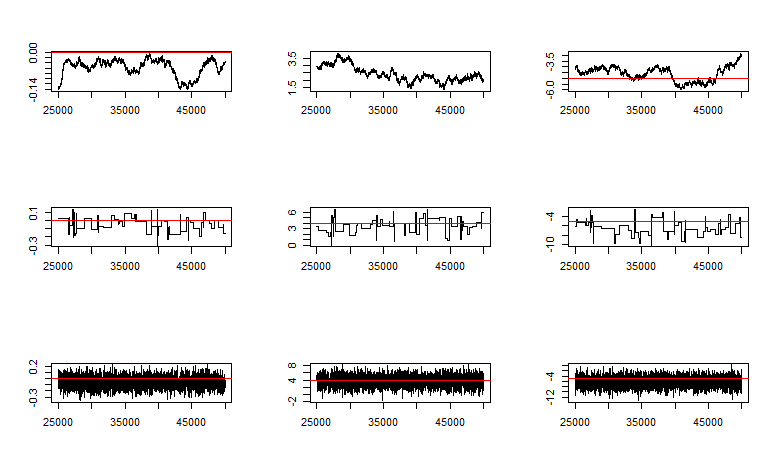
\includegraphics[width=\linewidth]{figures/probit_mcmc.png} 


Chains obtained for  $3$ values of  $\tau$ (resp. 0.01,1.5,10). We remove a burn-in period (25000 iterations over the total 50000 iterations)
\end{frame}


%====================================================================
\begin{frame}[fragile]\frametitle{Remarks}
 \begin{itemize}
  \item Target an acceptance rate of  25 \% in problems of small dimension, 50\% in large dimension problems. 
  \item Can also consider mixtures of kernels
$\rho_1 < \rho_2 < \rho_3$

$$\xi  \sim p_1 \mathcal{N}(0,\rho_1) + p_2 \mathcal{N}(0,\rho_2)+ (1-p_1-p_2) \mathcal{N}(0,\rho_3)$$
\item Be careful if the parameter leaves in a constrained set. 
\end{itemize}
\end{frame}


%====================================================================
\begin{frame}[fragile]\frametitle{Exercice}
 
Let us consider the Poisson regression : 
\begin{eqnarray*}
y_i &\sim& \mathcal{P}(\mu_i) \\
\log \mu_i &= & x_i \beta\\
\beta &\sim& \mathcal{N}(0, \sigma^2I_p) 
\end{eqnarray*}
 
\begin{itemize}
 \item Write (in R) a MCMC such that its asymptotic distribution is $p(\theta | y)$.
 \item Tune the size of the random walk to observe changes in the behavior
 \item See codes in \verb|BayesRegressionPoisson_MH.R|
\end{itemize}
  


 
\end{frame}



 




%====================================================================
\subsection[Gibbs]{Gibbs sampler} 
%==================================================================== 
\begin{frame}\frametitle{General Gibbs algorithm}
%====================================================================

If we want to sample a distribution  $p(\theta_1,\dots,\theta_d|\by)$  such that all the conditional distributions $g_j(\theta_1 | \theta_{\{-j\}},\by)$ are explicit, then the Gibbs algorithm is: 
\begin{block}{}
\begin{enumerate}
\item[] \vert Iteration 0:  \noir Initialize $\theta_1^{(0)} \dots, \theta_d^{(0)} $ 
\item[] \vert Iteration $m$ $(m=1\dots M)$: \noir  Given the current values of   $\theta_1^{(m-1)}, \dots, \theta_d^{(m-1)}$, 
\begin{itemize}
\item Simulate $\theta^{(m)}_1 \sim g_1(\theta_1 | \theta_2^{(m-1)}, \dots,x_d^{(m-1)},\by )$
\item Simulate  $\theta^{(m)}_2 \sim g_2(\theta_2 | \theta_1^{(m)}, \theta_3^{(m-1)}\dots,\theta_d^{(m-1)} ,\by)$
\item Simulate $\theta^{(m)}_3 \sim g_3(\theta_3 | \theta_1^{(m)},  \theta_2^{(m)}, \theta_4^{(m-1)}\dots,\theta_d^{(m-1)},\by)$
\item $\cdots$
\item  Simulate $\theta^{(m)}_d \sim g_d(\theta_d | \theta_1^{(m)}, \dots,\theta_{d-1}^{(m )},\by )$
\end{itemize}
\end{enumerate}
\end{block}
The stationary distribution is the joint one $p(\theta_1,\dots,\theta_p|\by)$



\end{frame}



%====================================================================
\begin{frame}\frametitle{Gibbs for latent variables}  
%====================================================================
Assume that we introduce latent variables $\bZ$ in the model such that   $[\bZ | \bY, \btheta]$ and  $[\btheta | \bY, \bZ]$  have an explicit form and can be easily simulated. 

\begin{block}{}
\begin{enumerate}
\item[] \vert Iteration 0:  \noir Initialise $\btheta^{(0)}$  et $\bZ^{(0)}$
\item[] \vert Iteration $m$ $(m=1\dots M)$: \noir  Given the current values of $\bZ^{(m-1)}$, $\btheta^{(m-1)}$
\begin{itemize}
\item Simulate $\bZ^{(m)} \sim [\bZ| \btheta^{(m-1)}, \bY]$
\item Simulate  $\btheta^{(m)} \sim [\btheta | \bZ^{(m)}, \bY]$
\end{itemize}
\end{enumerate}
\end{block}
We will get a sample of $(\bZ^{(m)}, \btheta^{(m)})_{m \geq 1}$ under the posterior distribution  $[\btheta, \bZ  | \bY]$ and so marginally $\btheta^{(m)} \sim [\btheta | \bY]$

\end{frame}

%====================================================================
\begin{frame}\frametitle{Exercice : Stationarity of $p(\theta,Z | Y)$}  
%====================================================================
\begin{enumerate}
 \item Explicit the kernel transition of the chain. 
 \item Prove that $p(\theta,Z | Y)$ is stationary.  
\end{enumerate}
\end{frame}

%====================================================================
\begin{frame}\frametitle{Convergence}  
%====================================================================
Ergodicity  and convergence studied in \cite{robert1999monte}.    

\end{frame}


%====================================================================
\begin{frame}\frametitle{Illustration : Gibbs sampler for a Poisson mixture model}
%====================================================================


\begin{itemize}
 \item  Mixture distribution 
 \begin{eqnarray*}
 Y_i &\sim&_{i.i.d.} \sum_{k=1}^K \pi_k \mathcal{P}(\mu_k)\\
  \end{eqnarray*}

\item Prior distribution
 \begin{eqnarray*}
 \mu_k &\sim& \Gamma(\alpha,\beta)\\
 \pi &\sim& \mathcal{D}ir(\nu, \dots, \nu)
 \end{eqnarray*}
 
\item Posterior distribution
$$[\pi, \mu_1, \dots \mu_K | Y] \propto \prod_{i=1}^n\left(\sum_{k=1}^K \pi_k e^{-\mu_k} \frac{\mu_k^{Y_i}}{Y_i!}\right) \prod_{k=1}^K\pi_k^{\nu-1}  \prod_{k=1}^K \mu_k^{\alpha-1} e^{-\beta \mu_k}
$$ 

\centering 

 \vert Not explicit
 
\end{itemize}
\end{frame}

%====================================================================
\begin{frame}\frametitle{Gibbs sampler for a Poisson mixture : latent variable version}
%====================================================================
\begin{itemize}
   \item Latent variables version
  \begin{eqnarray*}
 Y_i | Z_i = k &\sim&_{i.i.d.} \mathcal{P}(\mu_k)\\
 P(Z_i = k) &=& \pi_k\\
 (Z_{i1}, \dots,Z_{iK}) &\sim & \mathcal{M}(1, \pi) 
 \end{eqnarray*}
 with $Z_{ik} = \ind_{Z_i = k}$
 \item Conditional posterior distributions
\begin{equation*}
 \begin{array}{ccccl}
p(\mu,\pi | Y, Z) &\propto& p(Y,Z,\mu,\pi) &=& p(Y | Z, \mu) p(Z | \pi) p(\mu)  p(\pi)\\
p(Z | Y, \mu,\pi ) &\propto& p(Y,Z,\mu, \pi) &=& p(Y | Z, \mu) p(Z | \pi) \cancel{p(\theta)} \\
 \end{array}
\end{equation*}
\end{itemize}
\end{frame}

%====================================================================
\begin{frame}\frametitle{Gibbs sampler for a Poisson mixture: $p(\mu | Y,Z)$}
%====================================================================
 
 $$p(\mu | Y,Z) \propto p(Y | Z;\mu)   p(\mu)$$
 
 \begin{itemize} 
  \item \vert $ p(Y | Z, \mu)$ \noir 
 \begin{eqnarray*}
p(Y|Z,\mu) &=& \prod_{i=1}^n \frac{1}{Y_i!}e^{- \mu_{Z_i}} \mu_{Z_i}^{Y_i}\quad \pause  \propto \quad \prod_{k=1}^K \prod_{i=1,  Z_ik = 1}^n e^{- \mu_{k}} \mu_{k}^{Y_i}\pause \\
%&\propto&\prod_{k=1}^K  \left(e^{- \mu_{k}\sum_{i=1}Z_{ik}}\right)  \mu_{k}^{\sum_{i=1}Z_{ik}Y_i}\pause \\
&\propto&\prod_{k=1}^K e^{- \mu_{k}N_k}\mu_{k}^{S_k}
 \end{eqnarray*}
 with $N_k =\sum_{i=1}^nZ_{ik}$, $S_k = \sum_{i=1}^nZ_{ik}Y_i$ 
 
 \item \vert $p(\mu)$ \noir
 $$p(\mu) \propto \prod_{k=1}^K \mu_k^{\alpha-1} e^{-\beta \mu_k}$$
 
 \end{itemize}
 \end{frame}
 
%====================================================================
\begin{frame}\frametitle{Gibbs sampler for a Poisson mixture: $p(\mu | Y,Z)$}
%====================================================================
 
 $$p(\mu | Y,Z) \propto p(Y | Z;\mu)   p(\mu)$$
 
 
\begin{eqnarray*}
p(\mu | Y,Z) &\propto& \prod_{k=1}^K e^{- \mu_{k}N_k}\mu_{k}^{S_k}\prod_{k=1}^K \mu_k^{\alpha-1} e^{-\beta \mu_k}\\
&\propto& \prod_{k=1}^K e^{- \mu_{k}(N_k+\beta)}\mu_{k}^{\alpha + S_k-1}\\
\mu_k | Z,Y &\sim&_{i.i.d.} \Gamma(\alpha + S_k-1, N_k+\beta)
\end{eqnarray*}
 
\end{frame}
 
%====================================================================
\begin{frame}\frametitle{Gibbs sampler for a Poisson mixture: $p(\pi | Y,Z)$}
%====================================================================


$$ p(\pi | Y,Z) \propto  p(Z | \pi) p(\pi)$$

\begin{itemize}
\item \vert $ p(Z | \pi)$\noir 
   \begin{eqnarray*}
p(Z | \pi) &=& \prod_{i=1}^n \pi_{Z_i} \prod_{k=1}^K\prod_{i=1  | Z_{ik}=1}^n \pi_k \propto    \prod_{k=1}^K \pi_k^{N_k}
 \end{eqnarray*}
\item \vert $ p(\pi)$\noir 
$$p(\pi)\propto  \prod_{k=1}^K \pi_k^{\nu-1}$$
\item \vert $ p(\pi | Y,Z)  $\noir 
\begin{eqnarray*}
 p(\pi| Y,Z) &\propto& \prod_{k=1}^K \pi_k^{N_k + \nu-1}\\ 
 \pi  | Y,Z &\sim& \mathcal{D}ir(\nu +N_1, \dots, \nu + N_K)
\end{eqnarray*}
\end{itemize}
 \end{frame}

%====================================================================
\begin{frame}\frametitle{Gibbs sampler for a Poisson mixture: $p(Z | Y, \theta)$}
%====================================================================

\begin{itemize}
 \item 
\begin{eqnarray*}
p(Z | Y,\theta) &\propto&  p(Y | Z, \mu) p(Z | \pi) \\
&\propto& \prod_{i=1}^n e^{- \mu_{Z_i}} \mu_{Z_i}^{Y_i}  \pi_{Z_i}
\end{eqnarray*}
\item $Z_i$ independent conditionnally to $Y$ and $Z_i \in \{1, \dots, K\}$
\item 
\begin{eqnarray*}
   P(Z_i = k | Y,\theta)&\propto&  e^{- \mu_{k}} \mu_{k}^{Y_i}  \pi_{k}\\
   & = &  \frac{e^{- \mu_{k}} \mu_{k}^{Y_i}  \pi_{k}}{\sum_{k'=1}^K e^{- \mu_{k'}} \mu_{k'}^{Y_i}  \pi_{k'}}
\end{eqnarray*}
\end{itemize}
\end{frame}

 
%====================================================================
\begin{frame}\frametitle{Gibbs sampler for a Poisson mixture}
%====================================================================
\begin{block}{}
\begin{enumerate}
\item[] \vert Iteration 0:  \noir Initialize $\theta^{(0)}$  et $Z^{(0)}$
\item[] \vert Iteration $m$ $(m=1\dots M)$: \noir  Given current values of $Z^{(m-1)}$, $\theta^{(m-1)}$
 \begin{itemize}
 \item Simulate $ Z^{(m)} \sim [ Z| \theta^{(m-1)},  Y]$
 $\forall i=1,\dots,n$, $\forall g=1,\dots, G$
 \begin{eqnarray*}
   P(Z_i = k | Y,\theta^{(m-1)})&\propto&  e^{- \mu^{(m-1)}_{k}} (\mu^{(m-1)}_{k})^{Y_i}  \pi^{(m-1)}_{k}\\
  \end{eqnarray*}
%  }
 \item Simulate  $\theta^{(m)} \sim [\theta |  Z^{(m)},  Y]$
 {\scriptsize 
  \begin{itemize}
  \item  $N^{(m)}_k = \sum_{i=1}^n \ind_{Z^{(m)}_i=k}$ et  $S^{(m)}_{k} = \sum_{i=1}^n \ind_{Z^{(m)}_i=k}Y_{i}$
  \item  $ \mu^{(m)}_{k} | Z^{(m)},Y  \sim \Gamma\left(\alpha + S^{(m)}_{k}, b + N^{(m)}_k\right)$
  \item $ \pi^{(m)} | Z, Y  \sim \mathcal{D}ir(N^{(m)}_1 + \nu ,\dots,N^{(m)}_K + \nu) $
 \end{itemize}}
\end{itemize}
 \end{enumerate}
 \end{block}
  \end{frame}
  
%==================================================================== 
  \begin{frame}\frametitle{Exercice}
%====================================================================
Write the Gibbs corresponding to the SBM model
 $$Y_{ij} | Z_i = k, Z_j = l \sim \mathcal{P}(\mu_{kl})\quad , \quad P(Z_i = k) = \pi_k$$
\begin{enumerate}
 \item Write  the complete likelihood
 \item Propose prior distributions
 \item Calculate $P(\mu_{kl} | Y,Z)$
 \item Calculate $P(\pi | Y,Z)$
\item Are the $Z_i$'s independant conditionnally to $Y$? How will you proceed?  
 \end{enumerate}

  \end{frame}


%====================================================================
\begin{frame}\frametitle{Remarks on the Gibbs sampler}
%====================================================================
\begin{itemize}
\item For multidimensional distributions
\item Does not work if the number of parameters is variable % (ici, nombre de groupe $G$ fixé)
\item Constraining on the conditional distributions  (have to be explicit)
\item No tuning of the algorithm: + and -
\end{itemize}


\vspace{1em}


\color{dgreen}{Visualization}
\href{https://chi-feng.github.io/mcmc-demo/app.html?algorithm=GibbsSampling&target=banana}{\beamergotobutton{chi-feng interactive MCMC (Gibbs)}}
\end{frame}

  


%====================================================================
\subsection{Metropolis-Hastings within Gibbs}   
%====================================================================


%====================================================================
\begin{frame}\frametitle{Metropolis-Hastings within Gibbs} 
%====================================================================

 Convenient for latent variable models. Gibbs and Metropolis-Hastings combined
 
 \begin{block}{}
\vert Iteration 0:  \noir Initialise $\theta^{(0)}$  et $\bZ^{(0)}$\\

\vert Iteration $m$ $(m=1\dots M)$: \noir  Given the current values of $\bZ^{(m-1)}$, $\theta^{(m-1)}$
\begin{itemize}
 \item On the latent variables $\bZ$
        \begin{itemize}
        \item Propose $\bZ^{(c)} \sim q(\bZ| \bZ^{(m-1)},\theta^{(m-1)})$
        \item Accept with probability such that $[\bZ  |\theta  , \bY]$ is the stationary distribution 
        \end{itemize}
\item For each component of $\theta$
         \begin{itemize}
          \item Propose $\theta_k^{(c)} \sim q(\theta_k| \theta^{(m-1)}_{-\{k\}}, \bZ^{(m)})$
            \item Accept with probability such that $[\theta_k |\theta_{-\{k\}}, \bZ, \bY]$ is the stationary distribution  %$\theta_k \sim [\theta | \bZ^{(m)}, \bY]$
        \end{itemize}
\end{itemize}
\end{block}
We will get a sample of $(\bZ^{(m)}, \theta^{(m)})_{m \geq 1}$ under the posterior distribution  $[\btheta, \bZ  | \bY]$ and so marginally $\theta^{(m)} \sim [\theta | \bY]$

 \end{frame}
  
%====================================================================
 \begin{frame}{ Great but and now...}
%==================================================================== 
 \begin{itemize}
  \item Many packages to automatically construct the MCMC from your model. 
  \item Very flexible and adapted to latent variable models
  \item Based on the writing of the model : automatically designed proposals
 \end{itemize}
 
  \end{frame}
  
%====================================================================
\begin{frame}{Software}
%====================================================================
\begin{itemize}
  \item \href{http://www.mrc-bsu.cam.ac.uk/software/}{WinBUGS} : Bayesian inference Using Gibbs Sampling for Windows.  `Point-and-click’ windows interface version. May also be called from   
\includegraphics[width=0.05\linewidth]{figures/Rlogo-1.png}.  
  \item  With    
\includegraphics[width=0.05\linewidth]{figures/Rlogo-1.png} : package \textsf{R2WinBUGS}
  \item  \href{http://www.openbugs.net/w/FrontPage}{OpenBUGS} 
 \item \href{http://mcmc-jags.sourceforge.net/}{JAGS} : Just An Other Gibbs Sampler. More recent.From   
\includegraphics[width=0.05\linewidth]{figures/Rlogo-1.png}: r2JAGS or rJAGS...
 \item \href{https://mc-stan.org/}{STAN} : developed by Andrew Gelman, coding more complex but more powerful. 
 \end{itemize}
  
 \end{frame}
 
%====================================================================
\begin{frame}{In pratice}
%====================================================================
 \centering

Have a look at the file  
exempleLinearModelIrispresentation.html

 

  
\end{frame}
  
%====================================================================
\subsection{Tuning and assessing the convergence of MCMC}
%====================================================================
\begin{frame}{Tunning}
 
\begin{itemize}
 \item As we saw : step-size will have a non-neglectable influence on the convergence. 
 \item Solution : run the algorithm for a few iterations, check the acceptance rate 
\begin{itemize}
  \item If the acceptance rate is too low, decrease the step-size. 
  \item If the acceptance rate is too high, increase the step-size. 
\end{itemize}
\item \color{dgreen} \textbf{Be careful}\color{black}: not possible to adapt the acceptance rate   along the iterations, because in that case, it would not be a Markov Chain anymore (theoretical convergence conditions do not hold anymore)
\end{itemize}
\end{frame}


%====================================================================
\begin{frame}{Burn-in}
%====================================================================
\begin{itemize}
 \item Period where the chain will reach the stationary distribution
 \item Need to remove the first iterations (check the traces to calibrate)
\end{itemize}
 
\end{frame}
%====================================================================
\begin{frame}{Thinning}
 %====================================================================
\begin{itemize}
 \item With our sample $\theta^{(1)}, \dots, \theta^{(M)}$ we want to compute expectations, kernel density estimates of the posterior, etc...
 $$ \frac{1}{M}\sum_{m=1}^M \phi(\theta^{(m)})$$
 \item The convergence of such estimates is ensured (LGN) if the $\theta^{(m)}$ are independent and identically distributed.  
 \item In our case : $\theta^{(m)}$ realisations of a Markov Chain, so not independent. 
 \item To break the dependence, \color{dgreen} \textbf{thin}\color{black}: take one realization over ... (to be set). 
 \end{itemize}

\end{frame}
%====================================================================
\begin{frame}{Number of iterations}
%====================================================================
Must take into account

\begin{itemize}
 \item The complexity of the model (number of parameters to sample)
 \item The burn-in period you need
 \item The thinning parameter you need
 \item The time you have
\end{itemize}
From 10000 to \dots  millions?
\end{frame}
%====================================================================
\begin{frame}{Assessing convergence}
%====================================================================
\begin{itemize}
 \item Plot of the chains, parameter by parameter
 \item Plot the autocorrelations plots
 \item Compute numerical indicators
\end{itemize}

\end{frame}
%====================================================================
\begin{frame}{Gelman-Rubin convergence diagnostic}
%====================================================================
\begin{itemize}
 \item Relies on several chains run in parallel
 \item Let $c$ be the index for the chain. 
  \item Must be initialized from \emph{over dispersed initial values $\theta^{c(0)}$} with respect to the targeted distribution. 
  \item Formulae compare the variances intra and inter chains
   \begin{itemize}
  \item Within-chain variance  averaged over the chains:
  $$s^2_c = \frac{1}{M-1}\sum_{m=1}^M (\theta^{c(m)}- \overline{\theta^{c}})^2 \quad W = \frac{1}{C}\sum_{c=1}^C s^2_c$$
  \item Between-chain variance:  $$B = \frac{M}{C-1} \sum_{c = 1}^C (\overline{\theta^{c}} - \overline{\overline{\theta}})^2$$  
  \item Variance of $\theta | y$ is estimated as a weighted mean of these two quantities
  $$\widehat{\mbox{var}}\!(\theta|y)
= \frac{M-1}{M}\, W \, + \, \frac{1}{M} \, B.$$ 
\item \emph{Potential scale reduction statistic} is defined by
$$\hat{R}
\, = \,
\sqrt{\frac{\widehat{\mbox{var}}\!(\theta|y)}{W}}.$$

\item If all chains are at equilibrium $\hat{R} \approx 1$. Otherwise, if the chains have not converged to a common distribution, the  
$\hat{R} \geq 1$
\item \fbox{Compare $\hat{R}$ with $1.1$.}
\end{itemize}
\end{itemize}
\end{frame}
%====================================================================
\begin{frame}{Geweke convergence diagnostic}
%====================================================================
\begin{itemize}
 \item  Perform a test on two parts of the chain. 
 \item Assume that the chain is of $M$ iterations
 \item Take $M\alpha_1$  first iterations and $M \alpha_2$ last iterations (such that $\alpha_1 + \alpha_2 <1$  
\item Compute the mean of $\theta$ on the two parts
 \item If we are at the stationary distribution, then the two means should be equal
 \item Correction by the variances (taking into account the dependance between the realisations
 \item Geweke is the $Z$-statistic of the test.
 \item A z-score higher than the absolute value of 1.96 is associated with a p-value of < .05 (two-tailed). The absolute value of $Z$ should therefore be lower than  1.96.
 \end{itemize}
\end{frame}


%!TEX root = donnet_bayesianLVM_main.tex
\section[Deterministic approx.]{Deterministic approximation of the posterior distribution}


\subsection{Variational Bayes}

%################################################
\begin{frame}{Approximating the posterior : variational Bayes}
 
In a latent variable model, one wants to approximate
$p(\bZ, \theta | \by)$. 

\begin{itemize}
 \item Denote $\tilde{q}(\bZ, \theta)$ the approximation of $p(\bZ, \theta | \by)$. 
 \item We want to minimize
 $$ KL\left(\tilde{q}(\bZ, \theta), p(\bZ, \theta | \by)\right)$$
 where $KL$ is the Kullback Leibler divergence
 \item \vert Essential identity \noir
 $$ \underbrace{\log p(\by)}_{Cste} = KL\left(\tilde{q}(\bZ, \theta), p(\bZ, \theta | \by)\right) + \int \tilde{q}(\bZ, \theta) \log \frac{p(\by, \bZ, \theta)}{\tilde{q}(\bZ, \theta)} d\theta d\bZ$$
 \item Minimizing  $KL$ is equivalent to maximizing $$J(\by,\tilde{q}(\bZ, \theta))  = \int \tilde{q}(\bZ, \theta) \log \frac{p(\by, \bZ, \theta)}{\tilde{q}(\bZ, \theta)} d\theta d\bZ$$ 
 
 
 \end{itemize}
\end{frame}

%################################################
\begin{frame}{Approximating the posterior : variational Bayes}
$$J(\by,\tilde{q}(\bZ, \theta))  = \int \tilde{q}(\bZ, \theta) \log \frac{p(\by, \bZ, \theta)}{\tilde{q}(\bZ, \theta)} d\theta d\bZ$$ 

 \begin{itemize}
 \item $\log  p(\by, \bZ |  \theta) $ is explicit in a latent model
\item \vert \ Key point  \noir  Choose $\tilde{q}(\bZ, \theta)$ such that $J(\by,\tilde{q}(\bZ, \theta))$ can be computed explicitely. 
\end{itemize}
 
\end{frame}

%################################################

\begin{frame}{Approximating the posterior}

\begin{itemize}
 \item Mean field approximation:  $$\tilde{q}(\bZ, \theta) = \tilde{q}(\bZ) \tilde{q}( \theta)$$ (simplification)
 \item Alternatively maximize in $ \tilde{q}(\bZ)$ and $ \tilde{q}(\theta)$
 \item Minimizing a functional with respect to a function $\rightarrow$ Calculus of variations
 \item Equivalent to iterate
 
 \begin{enumerate}
 \item $\tilde{q}(\bZ) \propto \exp \left[\int \log  p(\by, \bZ |  \theta) \tilde{q}(\theta) d\theta \right]$
 \item $\tilde{q}(\theta) \propto \pi(\theta) \exp \left[\int \log  p(\by, \bZ |  \theta) \tilde{q}(\bZ) d\bZ \right]$
\end{enumerate}

\end{itemize}  

\end{frame}


% %################################################
% 
% \begin{frame}{Approximating the posterior}
% Maximise $J(\by, \tilde{q}(\bZ), \tilde{q}( \theta))$ with respect to both $\tilde{q}(Z)$ and
% $\tilde{q}( \theta)$ that play completely symmetric roles. We deal here with
% $q_Z$. In term the terms of Euler's problem, we have
% $$
% L(Z, q_Z) = q_Z(Z) \int q_\theta(\theta) \log \frac{P(Y, Z,
%   \theta)}{q_Z(Z) q_\theta(\thetabf)} \dd \theta.
% $$
% The solution must satisfy
% $$
% \frac{\partial L}{\partial q_Z} L(x, q_Z) 
% = \int q_\theta(\thetabf) \log P(Y, Z,
%   \thetabf) \dd \thetabf
% - \int q_\theta(\thetabf) \log q_\theta(\thetabf) \dd \thetabf
% - [\log q_Z(Z) - 1 ] \int q_\theta(\thetabf) \dd \thetabf
% = 0
% $$
% that is
% \begin{equation} \label{Eq:LnQZ}
%   \log q_Z(Z) = \int q_\theta(\thetabf) \log P(Y, Z, \thetabf)
%   \dd \thetabf  + \text{cst},
% \end{equation}
% so
% \begin{equation} \label{Eq:QZ}
%   q_Z(Z) \propto \exp \int q_\theta(\thetabf) \log
%   P(Y, Z, \thetabf) \dd \thetabf. 
% \end{equation}
% Similarly we get
% $$
% q_\theta(\thetabf) \propto \exp \int q_Z(Z) \log P(Y, Z, \thetabf) \dd
% Z
% $$
% so the two optimal distributions $q_Z$ and $q_\theta$ depend on each other.
% 
%  
%  
% 
% \end{frame}

%################################################

\subsection{Application}
\begin{frame}{Application to the Poisson mixture}

We consider the following  Poisson mixture model
\begin{eqnarray*}
Y_{i} | Z_i = k &\sim& \mathcal{P}(\mu_k)\\
P(Z_i = k) &=&  \pi_k\\ 
Z_{ik} &=& \ind_{Z_i=k}
\end{eqnarray*}

with the prior distributions: 

\begin{eqnarray*}
\mu_k &\sim& \Gamma(a_k,b_k)\\
(\pi_1, \dots, \pi_K) &\sim& \mathcal{D}ir(e_1, \dots, e_K)
\end{eqnarray*}

  
  
 \end{frame} 


%################################################

\begin{frame}{About $\tilde{q}(\theta)$}

{\footnotesize 
$\tilde{q}(\bZ) = \prod_{i=1}^n \tilde{q}_i(Z_i)$
with $\tilde{q}_i(Z_i=k) = \tau_{ik}$
\begin{eqnarray*}
\mathbb{E}_{\tilde{q}(Z)}\left[\log p(\by,\bZ | \theta) \right]&=& \sum_{i=1}^n \sum_{k=1}^K \tau_{ik}(-\mu_k + y_i \log \mu_k) +  \sum_{i,k} \tau_{ik} \log \pi_k + Cste\\
&=& \sum_{k}^K \left(-\mu_k \sum_{i=1}^n  \tau_{ik} + \log \mu_k \sum_{i=1}^n  \tau_{ik} y_i \right)+ \sum_{k=1}^K \log \pi_k \sum_{i=1}^n \tau_{ik} 
\end{eqnarray*}
So
\begin{eqnarray*}
\tilde{q}(\theta) &\propto& \pi(\theta) \exp \left[\mathbb{E}_{\tilde{q}(Z)}\left[\log p(\by,\bZ | \theta) \right]\right] \\
&\propto& \prod_{k=1}^K e^{-\mu_k \sum_{i=1}^n \tau_{ik} }\mu_k^{\sum_i y_i \tau_{ik}} \prod_{k=1}^K e^{-\mu_k b_k} \mu_k^{a_k-1} \pi_k ^{e_k-1}\\
&\propto& \underbrace{\prod_{k=1}^K \pi_k ^{\tilde{e}_k-1}}_{\mathcal{D}ir(\tilde{e}_1, \dots,\tilde{e}_K)} \prod_{k=1}^K  \underbrace{e^{-\tilde{b}_k \mu_k}  \mu_k^{\tilde{a}_k-1}}_{\Gamma(\tilde a_k, \tilde b_k)}
\end{eqnarray*}
with $$\tilde{e}_k = e_k + \sum_{i=1}^n \tau_{ik},\quad \tilde{a}_k  = a_k + \sum_{i=1}^ny_{i} \tau_{ik}\quad \tilde{b}_k  = b_k + \sum_{i=1}^n   \tau_{ik} $$ 
}

\end{frame}
%################################################

  \begin{frame}{About $\tilde{q}(\bZ )$}
  
  {\footnotesize 
  \begin{eqnarray*}
  &&\mathbb{E}_{\tilde{q}(\theta)}\left[\log p(\by,\bZ | \theta) \right]=\\
  &=& \sum_{i=1}^n \sum_{k=1}^K - Z_{ik}\mathbb{E}_{\tilde{q}(\theta)}[\mu_k] + Z_{ik} y_i \mathbb{E}_{\tilde{q}(\theta)}[\log \mu_k]  +  Z_{ik} \mathbb{E}_{\tilde{q}(\theta)}[\log \pi_k] + Cste \\ 
  &=&  \sum_{i=1}^n \sum_{k=1}^K  Z_{ik} \underbrace{ \left[-\frac{\tilde{a}_k}{\tilde{b}_k} + y_i \left[\Psi(\tilde{a}_k) - \log(\tilde{b}_k) +  \Psi(\tilde{e}_k)- \Psi(\overline{\tilde{e}})\right] \right]}_{\rho_{ik}}
  \end{eqnarray*}
   where $\Psi$ is the digamma function.
  }
  
  {\footnotesize 
  \begin{eqnarray*}
  \tilde{q}(\bZ) &\propto& \exp \left[\int \log  p(\by, \bZ |  \theta) \tilde{q}(\theta) d\theta \right]\\
  &\propto& e^{\sum_{i=1}^n \sum_{k=1}^K Z_{ik} \rho_{ik}}\\
  &\propto&\prod_{i=1}^n \prod_{k=1}^K (e^{\rho_{ik}})^{Z_{ik}}\\
  \tau_{ik} = P_{\tilde{q}(\bZ)}(Z_{ik}=1) &\propto& e^{\rho_{ik}}
  \end{eqnarray*}
  }
   
  \end{frame}
 
% %################################################
% 
\begin{frame}{Remarks on the methods}

  \begin{itemize}
   \item Algorithm (VBEM) iterates the two previously described steps.
   \item Optimization algorithm provides an approximation of the posterior distribution. 
    \item Quick but wrong
    \item Under-estimate the posterior variance
     \item If considering minimizing  
    $$ KL\left(p(\bZ, \theta | \by),\tilde{q}(\bZ, \theta)\right)$$ \vert $\Rightarrow $ \noir Expectation Propagation \href{https://en.wikipedia.org/wiki/Expectation_propagation}{EP on wikipedia} 
    \end{itemize}
    \end{frame}
%   ################################################
   \begin{frame}{Remarks in the implementation}
    
    \begin{itemize}
      \item Calculus adapted to each model. Less universal than MCMC. 
     \item Variational bayes  \textsf{R} Packages  : LaplacesDemon by Henrik Singmann \vert $\Rightarrow$ \noir Not working on our example
     \end{itemize}
   
  \end{frame}

  
  \subsection{Laplace Approximation}

  
  \begin{frame}{In a few words}
   
   
   \begin{itemize}
    \item Uses the  Laplace approximation  (Taylor extension around the MAP)
    \item OK for Gaussian Latent Model:
    \begin{eqnarray*}
     Y_i | x, \theta_2 &\sim& p(\cdot | x_i, \theta_2)\\
     x | \theta_1  &\sim& p(x | \theta_1) = \mathcal{N}(0,\Sigma)\\
     \theta = (\theta_1,\theta_2) &\sim& p(\theta)
    \end{eqnarray*}
  
  \item Many models are included
  
  \textbf{Exemple} : generalized linear model
 
 \begin{eqnarray*}
  Y_i &\sim& \mathcal{N}(\phi(\mu_i), \sigma^2)\quad   \mu_i = \alpha + \sum_{k=1}^K\beta_k z_{ki} \\
  x  = (\alpha,\beta_1, \dots,\beta_K) &\sim& \mathcal{N}(0,\Sigma)\\
  \theta_2   = \frac{1}{\sigma^2} &\sim&  \Gamma(a,b)
  \end{eqnarray*}
 
    
\item Particularly adapted to spatial models    
   \end{itemize}

   
  \end{frame}



%####################################################
\section{Importance sampling and Sequential Monte Carlo}
%####################################################
\subsection{Importance sampling : basics}
%####################################################
\begin{frame}[allowframebreaks]\frametitle{Importance sampling}
%####################################################


\begin{itemize}


\item For any function  $\varphi$ (...), $$E_{\theta | \bY} [\varphi(\theta)] = \int_\Theta \varphi(\theta) \vert \pi(\theta|\bY) d\theta\noir = \int_\Theta \varphi(\theta) \frac{\pi(\theta|\bY)}{\eta(\theta)}\vert \eta(\theta) d\theta\noir  $$
\item with  $\eta$ easily simulable distribution, such that its support contains the one of $\pi(\theta|\bY)$,  whose density can be computed.  
\end{itemize} 
 \framebreak
 

\vert  Monte Carlo estimator \noir  : $\theta^{(1)}, \dots , \theta^{(M)} \sim_{i.i.d.} \eta$
 
\begin{eqnarray*}
\widehat{E}_n[\varphi(\theta)] &=& \frac{1}{M}  \sum_{m=1}^M \frac{\pi(\theta^{(m)}| \bY)}{\eta(\theta^{(m)})}   \varphi(\theta^{(m)})\\&=&   \frac{1}{M}  \frac{1}{p(\bY)} \sum_{m=1}^M   \underbrace{\frac{ \ell(\bY | \theta^{(m)}) \pi(\theta^{(m)})}{ \eta(\theta ^{(m)})}}_{w^{(m)} }  \varphi(\theta^{(m)}) 
\end{eqnarray*}
 \vert But \noir  $p(\bY) $ without explicit expression:  $$p(\bY)  = \int  \ell(\bY | \theta) \pi(\theta)d\theta = \int \frac{ \ell(\bY | \theta) \pi(\theta)}{\eta(\theta)} \eta(\theta)d\theta  $$
$$\widehat{p(\bY)} =\frac{1}{M} \sum_{m=1}^n\frac{ \ell(\bY | \theta^{(m)}) \pi(\theta^{(m)})}{\eta(\theta ^{(m)})}  = \frac{1}{M}\sum_{m=1}^N w^{(m)}$$

  \begin{eqnarray*}
\widehat{E}_{\theta|\bY}[\varphi(\theta)] &=&  \frac{1}{M}  \sum_{m=1}^M  \frac{w^{(m)}}{p(\bY)} \varphi(\theta^{(m)})\\
\widehat{\widehat{E}}_{\theta | \bY} [\varphi(\theta)] &=& \frac{\cancel{\frac{1}{M}}  \sum_{m=1}^M  \rouge w_n^{(m)} \noir \varphi(\theta^{(m)})} { \cancel{\frac{1}{M}}  \rouge \sum_{m=1}^M  w^{(m)} \noir}\\
&=&   \sum_{m=1}^M  W^{(m)}  \varphi(\theta^{(m)})   \mbox{ avec } W^{(m)} = \frac{w^{(m)}}{ \sum_{m=1}^M w^{(m)}} 
\end{eqnarray*}
\begin{center}\vert Consistant Estimator \end{center}
\end{frame}

%####################################################
\begin{frame}\frametitle{Importance Sampling}
%####################################################

\begin{block}{Summary}
 Approximate $\pi(\theta | \bY)$ by a weighted sample $(\theta^{(m)}, W^{(m)})_{m=1\dots M}$ such that
$$ \theta^{(m)} \sim_{i.i.d.} \eta(\cdot)$$ 
$$W^{(m)} = \frac{w^{(m)}}{ \sum_{m=1}^M w^{(m)}}$$
$$ w^{(m)} = \frac{ \ell(\bY | \theta^{(m)}) \pi(\theta^{(m)})}{ \eta(\theta ^{(m)})}$$
\end{block}
\end{frame}


%####################################################
\begin{frame}{Importance Sampling: example}
%####################################################

\centering
 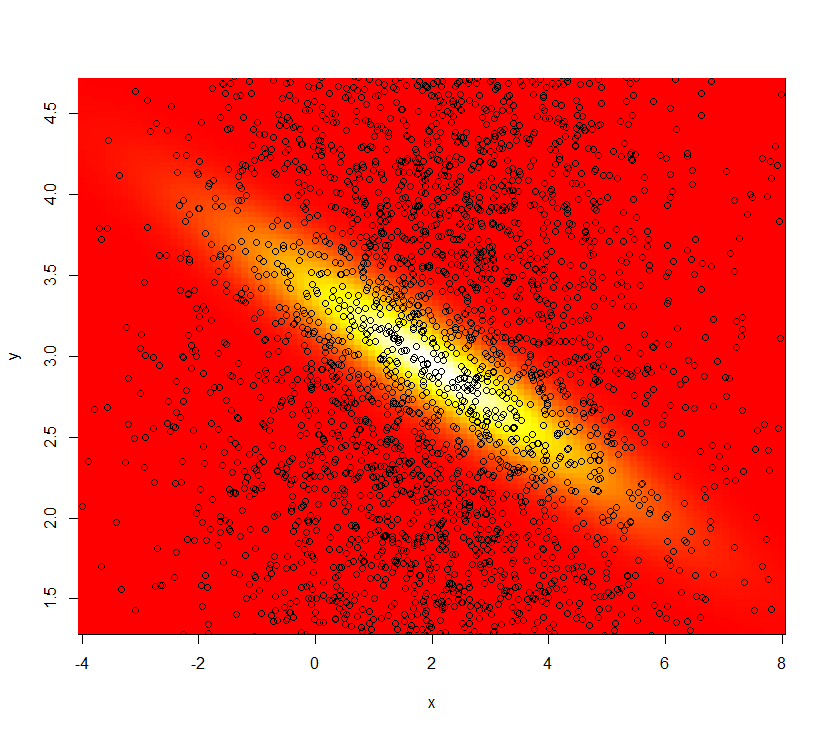
\includegraphics[width=0.8\textwidth]{figures/IS_sampling.png}
 
 Simulated particles, without their weights
 \end{frame}

 
%####################################################
 \begin{frame}{Importance Sampling: posterior}
%####################################################
 
\begin{figure}
   \begin{minipage}[c]{.46\linewidth}
 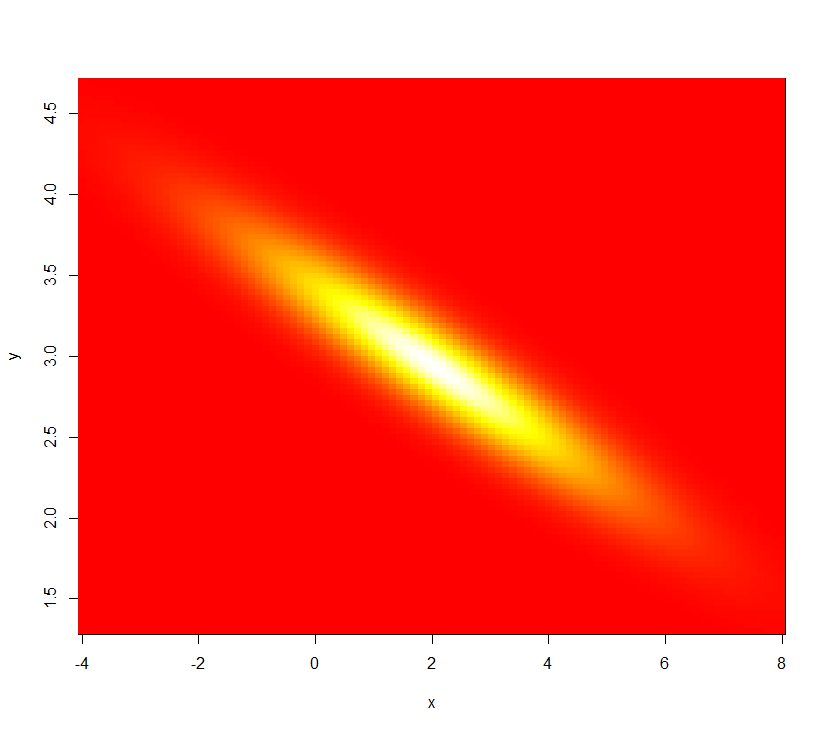
\includegraphics[width=\textwidth]{figures/post_2D_true.png}
   \end{minipage} \hfill
   \begin{minipage}[c]{.46\linewidth}
  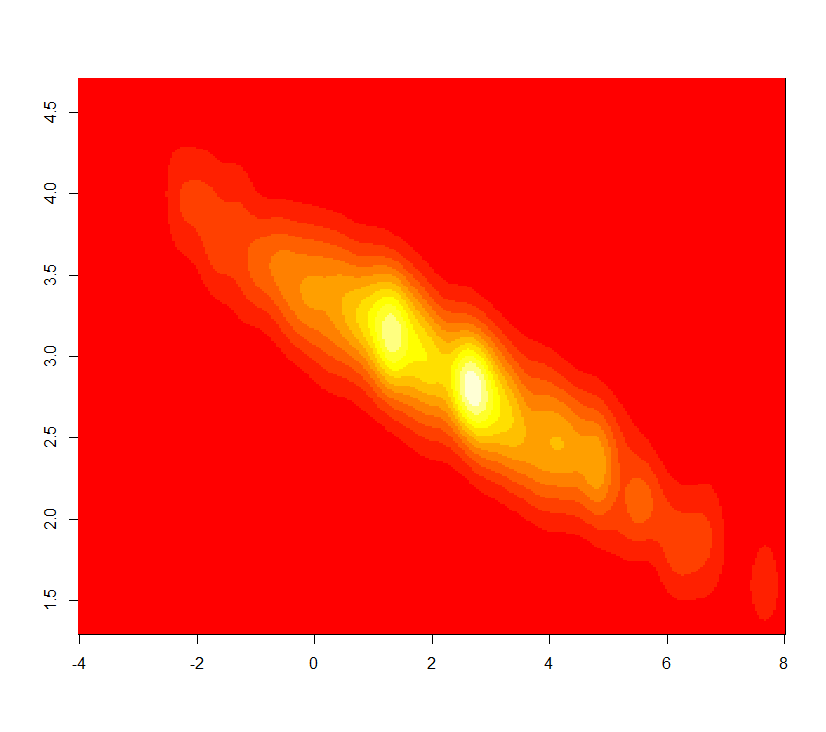
\includegraphics[width=\textwidth]{figures/post_2D_IS.png}
   \end{minipage}
   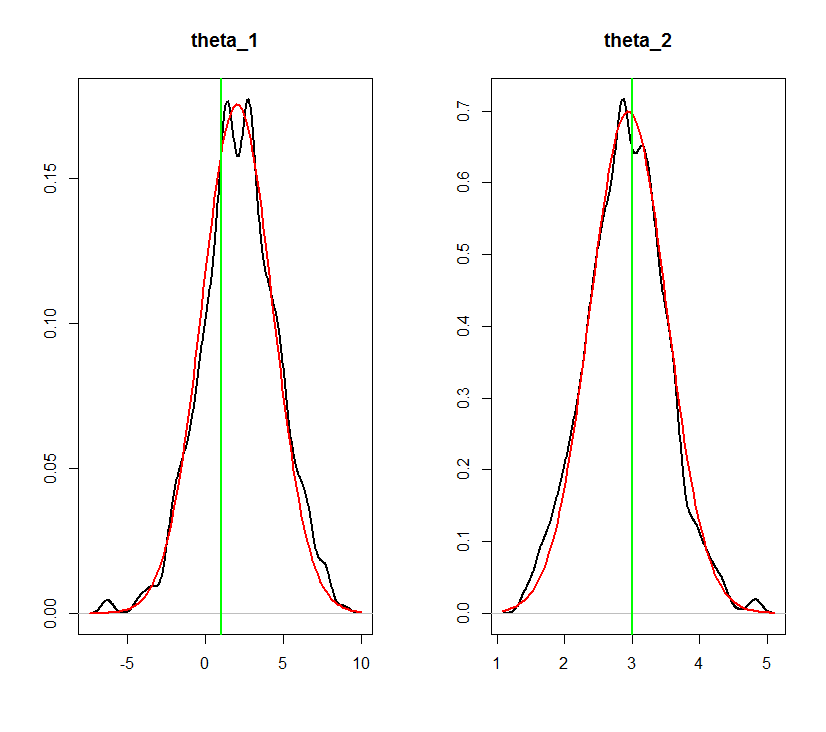
\includegraphics[width=\textwidth,height=3.8cm]{figures/post_IS_vraie.png}
\end{figure}
\end{frame}

%####################################################
\begin{frame}{Importance Sampling: an example that does not work}
%####################################################

\centering
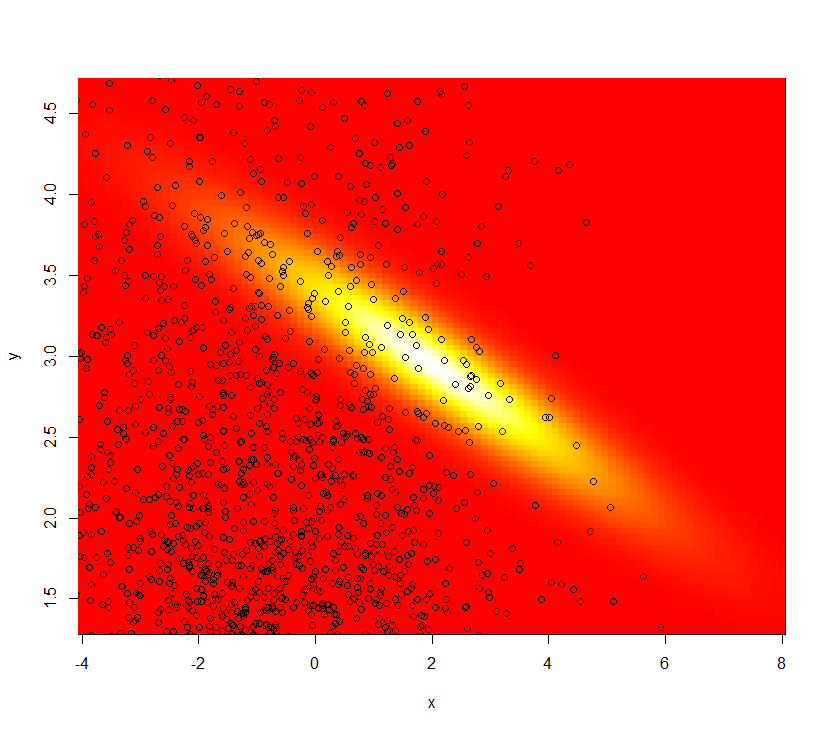
\includegraphics[width=0.8\textwidth]{figures/IS_sampling_2.png}
 
Simulated particles, without their weights 
\end{frame}

 
%####################################################
\begin{frame}{Importance Sampling: un example that does not work}
%####################################################
\begin{figure}
   \begin{minipage}[c]{.46\linewidth}
 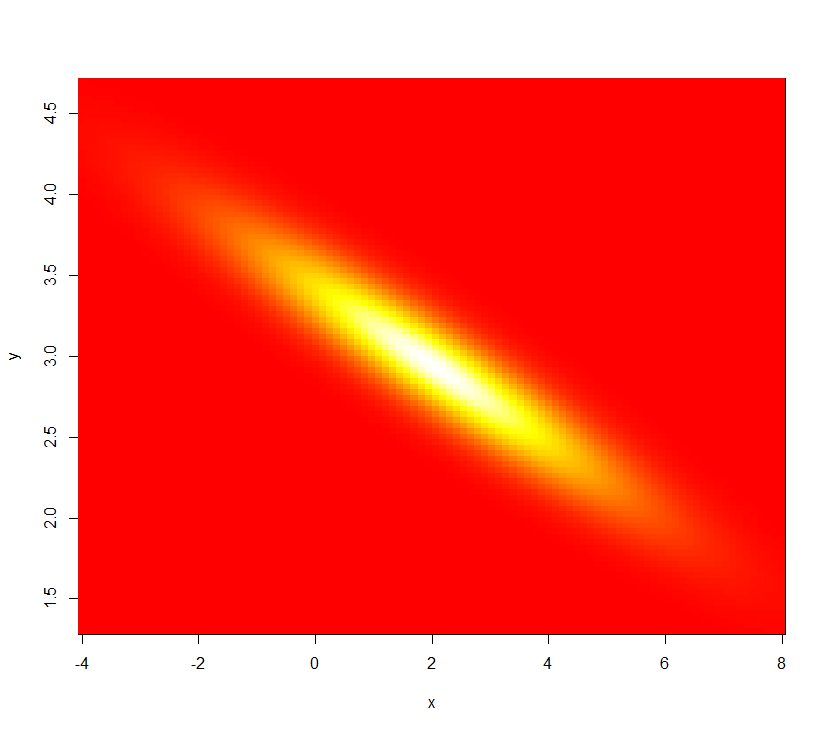
\includegraphics[width=\textwidth]{figures/post_2D_true.png}
   \end{minipage} \hfill
   \begin{minipage}[c]{.46\linewidth}
  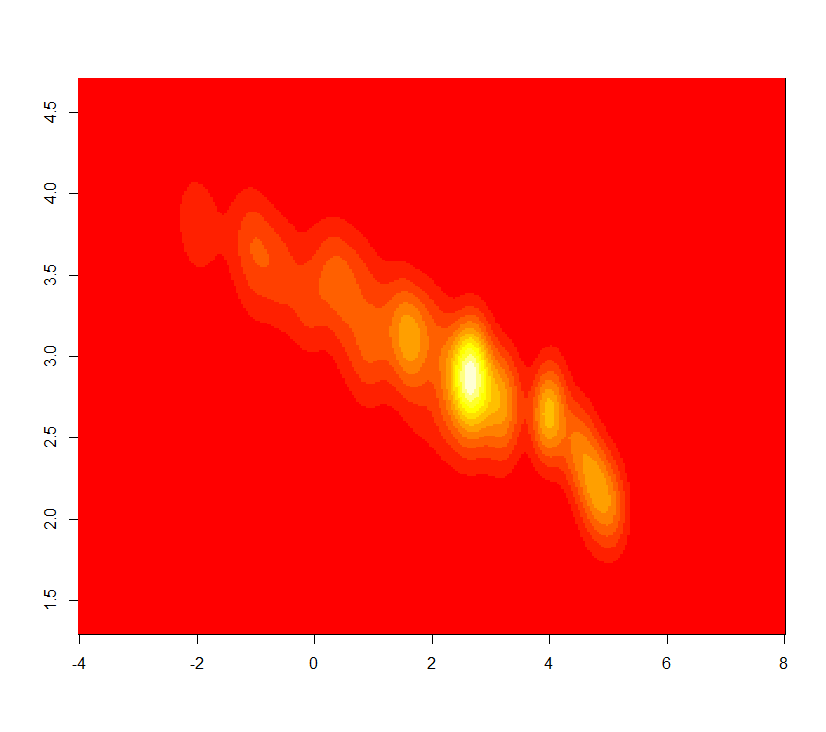
\includegraphics[width=\textwidth]{figures/post_2D_IS_2.png}
   \end{minipage}
   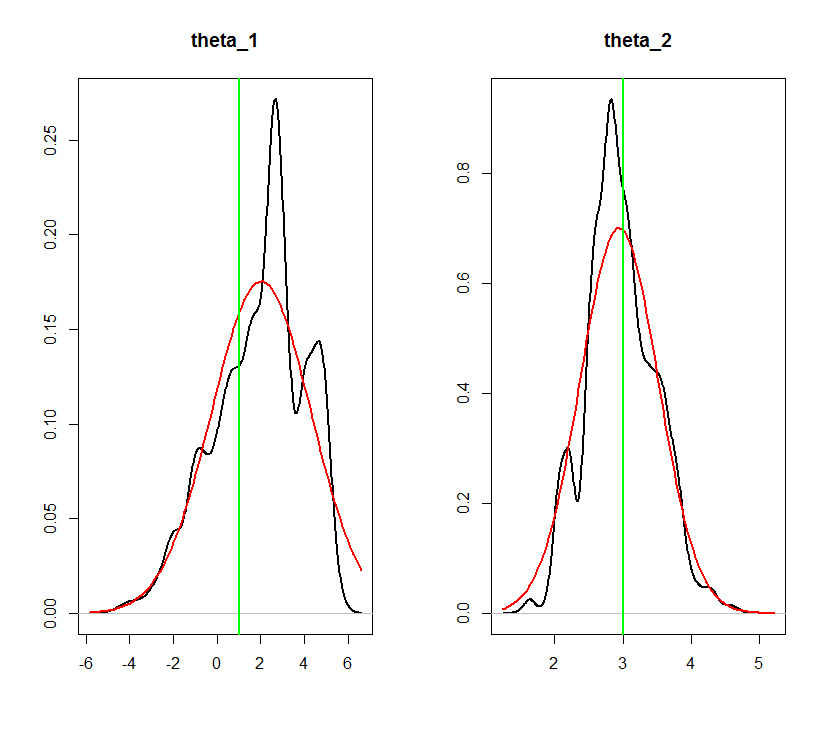
\includegraphics[width=\textwidth,height=3.8cm]{figures/post_IS_vraie_2.png}
\end{figure}
\end{frame}



%####################################################
 \begin{frame}[allowframebreaks=0.8]{Importance sampling methods: comments}
%####################################################

\begin{itemize}
\item Convergence ensured by the large numbers law. 
\item But the quality of the estimator (variance) for a given $M$ ?   
\item  Problem if some weights are very large while others are very small. 
\begin{itemize}
\item Calculus of the \vert Effective Sample Size\noir: 
$$ ESS = \frac{1}{ \sum_{m=M}^N \left(W^{(m)}\right)^2 }$$
\item $EES \in [1,M]$. 
\item The weighted sample $(W^{(m)},  \theta^{(m)})$  corresponds to a no-weighted sample of size  $ESS$ 
\end{itemize}
\item Essential to chose  $\eta$ carefully such that   $\ell(\bY| \theta^{(m)}) \pi(\theta^{(m)})$ not two small. 
\item Not possible in large dimension problems: need to sequentially build $\eta$ \vert Sequential Monte Carlo \noir
\item \vert Advantage: \noir easy estimation of $p(\bY)$ par $\sum_{m=1}^M w^{(m)}$
\end{itemize}
\end{frame}

%####################################################
\subsection[VB-IS]{Sequential Importance Sampling}
%####################################################
\begin{frame}\frametitle{}
%####################################################


\begin{block}{Problematic}
Can we use the variational approximation of the posterior distribution in a IS procedure. Can we correct its tendancy to under-estimate the posterior variance?  
\end{block}

Let  $\eta^{VB}$ be the VB posterior approximation of  $\pi(\theta|\bY)$. 

\begin{block}{Naive idea}
\begin{itemize}
\item IS using  $\eta_{VB}$ as a sampling distribution
\item  \vert But\noir : $\eta_{VB}$ has a support smaller than the one of  $\pi(\theta|\bY)$ 
\end{itemize}
\end{block}
\begin{block}{Naive idea 2}
\begin{itemize}
\item Using a dilated version of  $\eta_{VB}$
\item  Problems : how? how much? 
\item The problems of neglected dependencies remains
\end{itemize}
\end{block}

\end{frame}
%####################################################
\begin{frame}{IS with $\eta_{VB}$ }
%####################################################

\centering 
 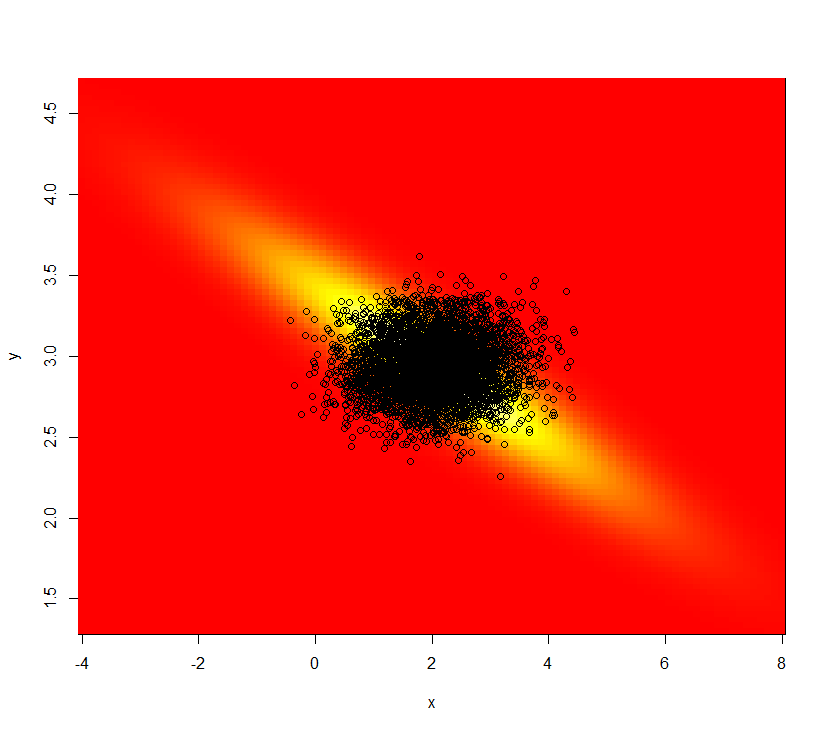
\includegraphics[width=0.8\textwidth]{figures/IS_sampling_VBEM.png}
 
 Particles simulated not weighted 
  \end{frame}
 %----------------------------------------------------------------------

%####################################################
\begin{frame}{IS with $\eta_{VB}$}
%####################################################

\begin{figure}
   \begin{minipage}[c]{.46\linewidth}
 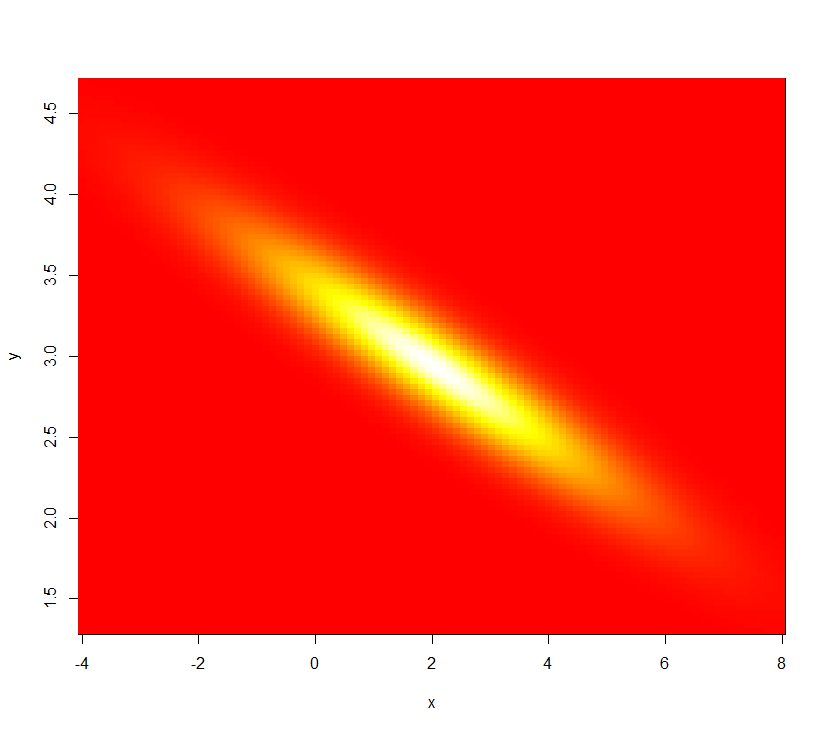
\includegraphics[width=\textwidth]{figures/post_2D_true.png}
   \end{minipage} \hfill
   \begin{minipage}[c]{.46\linewidth}
  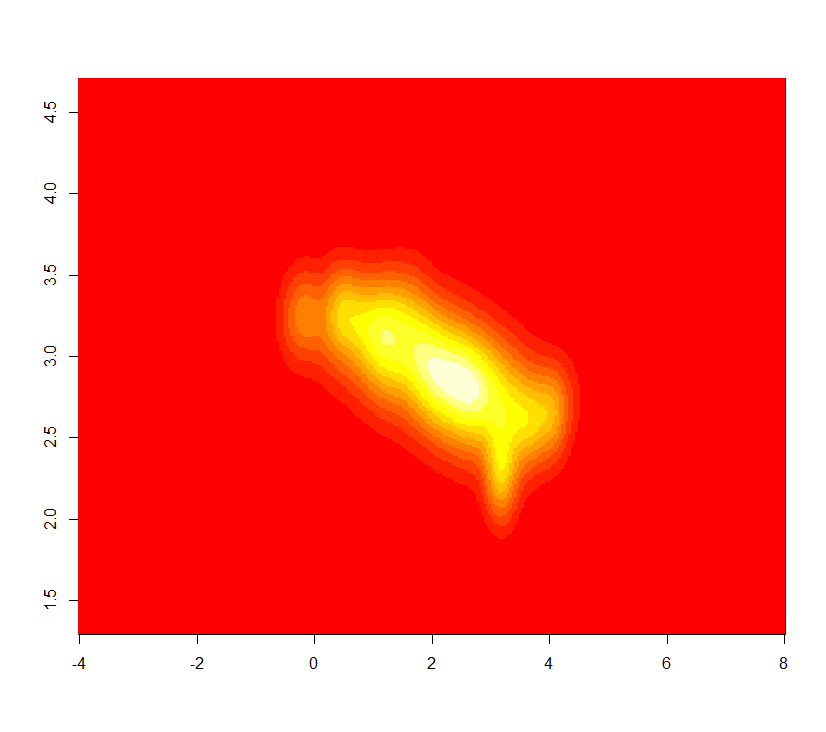
\includegraphics[width=\textwidth]{figures/post_2D_IS_VBEM.png}
   \end{minipage}
   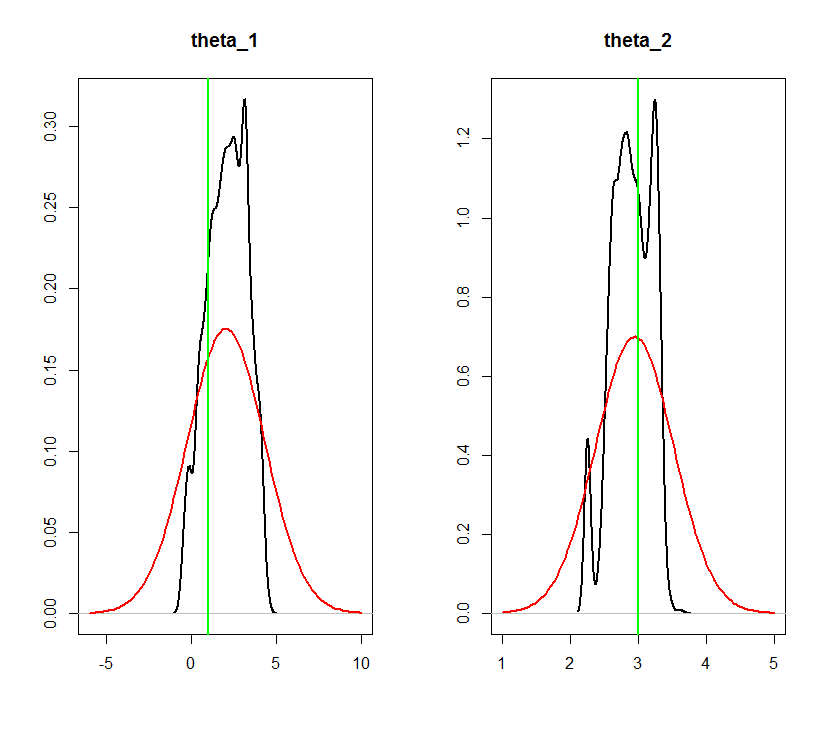
\includegraphics[width=\textwidth,height=3.5cm]{figures/post_IS_vraie_VBEM.png}
\end{figure}
\end{frame}



%####################################################
\begin{frame}\frametitle{One solution}
%####################################################


\begin{block}{Sequential sampling of a sequence of distributions} 
Let $\alpha_n$ be a increasing sequence such that
$\alpha_0 = 0  $ et $\alpha_N=1 $. 

Sample sequentially 
$$\pi_n(\theta)  \propto   \eta_{VB}(\theta)^{1- \alpha_n} (\ell(\bY | \theta) \pi(\theta))^{\alpha_n} = \frac{\gamma_n(\theta)}{Z_n}$$ 
using at each step  $n$  a sampling distribution  $\eta_n$ ``judicious''. 
\end{block}

\vert Remarks: \noir
\begin{itemize}
\item $\log\pi_n(\theta) = Cste +   (1- \alpha_n)  \log \eta_{VB}(\theta) + \alpha_n  \log (\ell(\bY | \theta) \pi(\theta))$
\item $n=0$ : $\pi_n(\theta)   =   \eta_{VB}(\theta)$.  Easy to simulate.  
\item $n=N$ : $ \pi_n(\theta)   \propto   \ell(\bY | \theta) \pi(\theta) = \pi(\theta| \bY)$: \vert goal reached
\item If $\alpha_n$ does not increase too fast $\pi_n(\theta) \approx \pi_{n+1}(\theta)$. 
 \end{itemize}
\end{frame}




%####################################################
\begin{frame}\frametitle{From $\eta_n$ to $\eta_{n+1}$}
%#################################################### 
 Assume that at itération $n$,  we have built  $\eta_n$ efficient for  $\pi_n$ :  $$\theta_n^{(1)}, \dots, \theta_n^{(M)} \sim \eta_n(\theta)$$ 
\vspace{1em}

At iteration  $n+1$,  we want to simulate  $\pi_{n+1}(\theta)$ using that previous sample
\begin{itemize}
\item \vert Intuition \noir: if $\pi_n \approx \pi_{n+1}$ simulate $\theta_{n}^{(m)}$ in a neighbourood of  $\theta_{n+1}^{(m)}$, i.e. using a Markovian kernel
$$ \theta_{n+1}^{(m)} | \theta_n^{(m)} \sim K_{n+1}(\theta_n^{(m)}, \theta_{n+1}^{(m)})$$
\item[] Example : $ \theta_{n+1}^{(m)} = \theta_n^{(m)} + \varepsilon_i$ with $\varepsilon_i \sim\mathcal{N}(0,\rho^2)$ 
\item  \vert New weights: \noir  $$w_{n+1}(\theta) = \frac{\gamma_{n+1}(\theta)}{\eta_{n+1}(\theta)} $$

\item \vert But \noir 
$$\eta_{n+1}(\theta_{n+1})  = \int_{\Theta}\eta_n(\theta_n) K _{n+1}(\theta_n,\theta_{n+1}) d\theta_n$$

\begin{center}
No explicit expression
\end{center}
\end{itemize}

\end{frame} 

%####################################################
\begin{frame}{After $N$ iterations}
%####################################################
\begin{itemize}
\item At iteration $0$,  simulate   $\theta_0^{(1)}, \dots, \theta_0^{(M)} \sim \eta_{VB}(\cdot) = \pi_0(\cdot)$ 
\item At iteration $1$,  use the instrumental distribution: 
$$\eta_{1}(\theta_{1})  = \int_{\Theta}\pi(\theta_0)  K_1(\theta_0,\theta_{1}) d\theta_0$$
\item At iteration $N$, use: 
$$\eta_{N}(\theta_{N})  = \int_{\Theta^{N-1}} \pi(\theta_0) \prod_{n=1}^{N}  K_n(\theta_{n-1},\theta_{n}) d\theta_{0:N-1}$$
 \end{itemize}
\end{frame}


%####################################################
\begin{frame}{SMC by \vert {\small \cite{delmoral06}}\noir}
%####################################################

\begin{itemize}
\item Prove that one can apply the previous algorithm without having to comptue  $\eta_{n}(\theta_{n})$
\item \vert Main idea  \noir:  introduce an atifical backward Markovian kernel  $L_{n-1}(\theta_n, \theta_{n-1})$ such that $\int_{\Theta} L_{n-1}(\theta_n, \theta_{n-1}) d\theta_{n-1} = 1$

\item Sample 
$$\widetilde{\pi}_n(\vert \theta_0,\dots,\theta_{n-1}, \noir \theta_n) =\pi_n(\theta_n)\prod_{k=0}^{n-1}L_{k}(\theta_{k+1}, \theta_{k})$$

\item By properties of the `backward'' kernel, the marginal version   of $ \widetilde{\pi}_n(\theta_0,\dots, \theta_n)$ is  $\pi_n$ 
{\scriptsize
\begin{eqnarray*}
\int_{\Theta ^{n-1}}\widetilde{\pi}_n( \theta_0,\dots,\theta_{n-1}, \theta_n) d\theta_{0:n-1} &=& \int_{\Theta^{n-1}} \pi_n(\theta_n)\prod_{k=0}^{n-1}L_{k}(\theta_{k+1}, \theta_{k})d\theta_{0:n-1}\\
&=& \pi_n(\theta_n) \underbrace{\int_{\Theta^{n-1}}\prod_{k=0}^{n-1}L_{k}(\theta_{k+1}, \theta_{k})d\theta_{0:n-1}}_{=1}
\end{eqnarray*}
}

\item $\widetilde{\pi}_n$ is defined on  $\Theta^n$, of increasing dimension at each iteration
\end{itemize}


\end{frame}

%####################################################
\begin{frame}{SMC by {\small \cite{delmoral06}}}
%####################################################
$$\widetilde{\pi}_n(\vert \theta_0,\dots,\theta_{n-1}, \noir \theta_n) =\pi_n(\theta_n)\prod_{k=0}^{n-1}L_{k}(\theta_{k+1}, \theta_{k}) = \frac{\widetilde \gamma_n(\theta)}{\widetilde Z_n}$$
\begin{itemize}
\item Assume that at iteration  $n-1$ we have  $\left\{ W_{n-1}^{(m)}, \theta^{(m)}_{1:n-1}\right\}$ approximating  $\widetilde{\pi}_{n-1}$

\item At time $n$, we propose $$\theta_{n}^{(m)} \sim K_n(\theta_{n-1}^{(m)}, \theta_{n}^{(m)})$$
\item $\eta_n(\theta_0, \dots,\theta_n) =  K_n(\theta_{n-1}, \theta_{n}) \eta_{n-1}(\theta_0, \dots,\theta_{n-1})$
\item  Un-normalized weights: 
\begin{eqnarray*}
w_{n}(\theta_{0:n})& =& \frac{\widetilde{\gamma}_n(\theta_{0:n})}{\eta_n(\theta_{0:n})} \\ 
&=&  \frac{\widetilde{\gamma}_{n-1}(\theta_{0:{n-1}})}{\eta_{n-1}(\theta_{0:n-1})} \vert \frac{L_{n-1}(\theta_{n}, \theta_{n-1})}{ K_n(\theta_{n-1}, \theta_{n})}\frac{\gamma_n(\theta_n)}{\gamma_{n-1}(\theta_{n-1})} \noir \\
&=&w_{n-1}(\theta_{0:n-1}) \vert \widetilde{w}_{n-1}(\theta_{n-1},\theta_n) \noir
\end{eqnarray*}

\end{itemize}

\end{frame}

%####################################################
\begin{frame}{Choosing $K_n$}
%####################################################
\begin{itemize}
\item\vert {Independant kernels} \noir : $$K_n(\theta_{n-1},\theta_n) = K_n(\theta_{n-1})$$
\vert $\Rightarrow$ \noir Poorly efficient for complicated distributions : no learning. 
\item \vert Local random network \noir : $$\theta_n = \theta_{n-1} + \mathcal{N}(0,\rho^2)$$
\vert $\Rightarrow$  \noir Choice of  $\rho^2$? Does not use  $\pi_n$ 
\item\vert MCMC type kernel \noir :  $K_n$ such that  $\pi_n$ is invariant. 
\begin{itemize}
\item If  $\pi_{n-1} \approx \pi_n$ and the chain moves fastly then we can hope  that $\eta_n \approx \pi_n$. 
\item But,  anyway, the divergence between  $\eta_n$ and $\pi_n$ is corrected. 
\item Allows to use practical knowledge and theory from  MCMC
\end{itemize}
\end{itemize}
\end{frame}



%####################################################
\begin{frame}{Choosing $L_{n-1}$}
%####################################################

\begin{itemize}
\item Purely artificial, but used to avoid the inegration against  $\eta_n$ when calculating the weights
\item Price to pay: increase of the domain  $\Theta \rightarrow \Theta^n$ and increasing of the weight variance
\item Possibility to give the expression of the optimal $L^{opt}_{n-1}$ minimizing the weigth variance $w_n(\theta_{0:n})$  (without explicit expression)
\item In practice, look for  $L_{n-1} \approx L^{opt}_{n-1}$ or the one simplifying the calculus
\end{itemize}
\end{frame}

%####################################################
\begin{frame}[allowframebreaks]{Choosing $L_{n-1}$ for a MCMC type kernel}
%####################################################
\begin{itemize}
\item For  $K_n$ MCMC-kernel of stationnary ditribution $\pi_n$,   on choose 
$$L_{n-1}(\theta_n,\theta_{n-1}) = \frac{\pi_n(\theta_{n-1}) K_n(\theta_{n-1},\theta_n)}{\pi_n(\theta_n)} =\frac{\gamma_n(\theta_{n-1}) K_n(\theta_{n-1},\theta_n)}{\gamma_n(\theta_n)}  $$
\item Then
\begin{eqnarray*}
\int_{\theta_{n-1}} L_{n-1}(\theta_n,\theta_{n-1}) d \theta_{n-1} &=& \frac{  \int_{\theta_{n-1}} \pi_n(\theta_{n-1}) K_n(\theta_{n-1},\theta_n)d \theta_{n-1}}{\pi_n(\theta_n)} \\
&=&  \frac{\pi_n(\theta_n)}{\pi_n(\theta_n)} \mbox{ by stationarity of $\pi_n$ /  $ K_n$ } \\
&=& 1 
\end{eqnarray*}

\item Consequences on the non-normalized weights
\begin{eqnarray*}
w_{n}(\theta_{0:n}) &=&w_{n-1}(\theta_{0:n-1})   \vert \frac{L_{n-1}(\theta_{n}, \theta_{n-1})}{ K_n(\theta_{n-1}, \theta_{n})}\frac{\gamma_n(\theta_n)}{\gamma_{n-1}(\theta_{n-1})} \noir \\
&=&w_{n-1}(\theta_{0:n-1})  \frac{ \gamma_n(\theta_{n-1}) }{\cancel{\gamma_n(\theta_n)}}\frac{\cancel{\gamma_n(\theta_n)}}{\gamma_{n-1}(\theta_{n-1})}  \\
&=& w_{n-1}(\theta_{0:n-1})\frac{ \eta_{VB}(\theta_{n-1})^{1- \alpha_n} (\ell(\bY | \theta_{n-1}) \pi(\theta_{n-1}))^{\alpha_n}}{ \eta_{VB}(\theta_{n-1})^{1- \alpha_{n-1}} (\ell(\bY | \theta_{n-1}) \pi(\theta_{n-1}))^{\alpha_{n-1}}}\\
&=& w_{n-1}(\theta_{0:n-1}) \left[\frac{\ell(\bY | \theta_{n-1}) \pi(\theta_{n-1})}{\eta_{VB}(\theta_{n-1})} \right]^{\alpha_n-\alpha_{n-1}} 
\end{eqnarray*}



\item Do not depend on  $\theta_n$ : can be computed before the move. 


\end{itemize}
\end{frame}




%####################################################
\begin{frame}\frametitle{Algorithm  SMC : initialization}
%####################################################

\begin{block}{Initialization :  $n=0$}
\begin{itemize}
\item Pour $m=1\dots N$, $\theta_0^{(m)} \sim _{i.i.d} \eta_{VB}(\cdot)$
\item Calculer $w_0^{(m)} =1 $ et  $W_0^{(m)}=\frac{1}{M}$. 
\end{itemize}
\end{block}

\end{frame}

\begin{frame}\frametitle{Algorithm SMC}
\begin{block}{At iteration $n$}

\begin{itemize}
\item $\forall m=1\dots M$, calculate $$w^{(m)}_n =w_{n-1}(\theta^{(m)}_{0:n-1}) \left[\frac{\ell(\bY | \theta^{(m)}_{n-1}) \pi(\theta^{(m)}_{n-1})}{\eta_{VB}(\theta^{(m)}_{n-1})} \right]^{\alpha_n-\alpha_{n-1}}  $$
\item Deduce $W_n^{(i)}$ and compute the effective sample size: $ESS(W_n^{(i)})$. 
\item If $ESS>seuil$ :   $\theta_n^{(m)} = \theta_{n-1}^{(m)}$
\item If $ESS<seuil$ : 
\begin{itemize}
\item \vert Resample:  \noir$\widetilde{\theta}_{n}^{(m)} \sim \sum_{i=1}^M W_n^{(i)}\delta_{\{\theta_{n-1}^{(i)}\}}$ and $w_n^{(m)}=1$ $\forall m=1\dots M$. 
\item \vert Propagation: \noir $\theta^{(m)}_n \sim K_n(\widetilde{\theta}_{n}^{(m)}, \cdot)$ where $K_n$ is made of a kew iterations of a MH of stationnary distribution  $\pi_n$. 
\end{itemize}
 
\end{itemize}
\end{block}
\end{frame}

%####################################################
\begin{frame}{Adaptative version}
%####################################################

At each iteration, push $\alpha_n$ until the ESS falls under a threshold  $ESS<seuil$. 

\begin{block}{At iteration $n$}
\begin{itemize}
\item Find  $\alpha_n$ such that: $\alpha_n = \inf_{\alpha > \alpha_{n-1}} \{ ESS_n(\alpha)<seuil\} $
with 
{\scriptsize $$w^{(m)}_{n,\alpha} =  \left[\frac{\ell(\bY | \theta^{(m)}_{n-1}) \pi(\theta^{(m)}_{n-1})}{\eta_{VB}(\theta^{(m)}_{n-1})} \right]^{\alpha-\alpha_{n-1}}, \quad W_{n,\alpha}^{(m)} =\frac{w^{(m)}_{n,\alpha}}{\sum_{m=1}^M w^{(m)}_{n,\alpha}}$$ 
$$  ESS_n(\alpha) = \frac{1}{ \sum_{m=M}^N \left(W_{n,\alpha}^{(m)}\right)^2 } $$}
\item \vert Re-sample: \noir$\widetilde{\theta}_{n}^{(m)} \sim \sum_{i=1}^M W_{n,\alpha_n}^{(i)}\delta_{\{\theta_{n-1}^{(i)}\}}$ and $w_n^{(m)}=1$  $\forall m=1\dots M$. 
\item \vert Propagate: \noir $\theta^{(m)}_n \sim K_n(\widetilde{\theta}_{n}^{(m)}, \cdot)$ where $K_n$ is made of a few iterations of a MH of stationnary distribution  $\pi_n(\theta)= \eta_{VB}(\theta)^{1- \alpha_n} (\ell(\bY | \theta) \pi(\theta))^{\alpha_n}$. 
 
\end{itemize}
\end{block}
\end{frame}






\subsection[Illustration]{Numerical illustration : toy example}

%####################################################
\begin{frame}{Simulated data}
%####################################################
\begin{itemize}
\item Mixture of 4-dimensional Bernoulli distributions
\item $n$ = number of individuals
\item $K$ = number of mixture components
\item $Y_{ij}$: observation of individual  $i$ of component $j$. 
\item $Z_{ik}$ : equal $1$ if $i$ belongs to  group  $k$. $Z_{i\;\bullet}=(Z_{i1},\dots,Z_{iK})$
\item $\forall i=1,\dots,n, \forall j=1\dots 4$ 
$$Y_{ij}| Z_{i\bullet} \sim_{i.i.d} \mathcal{B}ern(Z_{i\bullet} \gamma_{\bullet\; j})$$
$$P(Z_i=k) = \pi_k$$ 
\item $\theta=(\bpi , \gamma)$ with $\bpi = (\pi_1,\dots,\pi_K)$ and  $\gamma$ probability matrix of size  $K\times 4$
\end{itemize}
\end{frame}


%####################################################
\begin{frame}{Prior and variational posterior}
%####################################################
\begin{block}{Prior}
\begin{eqnarray*}
(\pi_1\dots,\pi_K) &\sim& \mathcal{D}(1,\dots,1),\quad d_k \in \mathbb{R}^{+*}\\
\gamma_{kj} &\sim&_{i.i.d.} \; \mathcal{B}(1,1),\quad (j,k) \in\{1,\dots,J\} \times \{1,\dots,K\}
\end{eqnarray*}
\end{block}

\begin{block}{Posterior distribution given by VBEM $\eta_{VB}(\btheta,\bZ | \bY)$} 
\begin{eqnarray*}
(\pi_1\dots,\pi_K) &\sim& \mathcal{D}ir(\widetilde{d}_1,\dots,\widetilde{d}_K),\quad \widetilde{d}_k \in \mathbb{R}^{+*}\\
\gamma_{kj} &\sim&_{i.i.d.} \; \mathcal{B}eta(\widetilde{a}_{kj},\widetilde{b}_{kj}),\quad (j,k) \in\{1,\dots,J\} \times \{1,\dots,K\}\\
\bZ_{i,\bullet} &\sim& \mathcal{M}ult(\widetilde{\tau}_{i\bullet}), \quad \sum_{i=1}^n \widetilde{\tau}_{ik} = 1
\end{eqnarray*}
\end{block}
\end{frame}

%####################################################
\begin{frame}{Tuning of the algorithm}
%####################################################

\begin{itemize}
\item $N=2000$ particles

\item Kernel $K_n$ : $5$ iterations of a standard Gibbs (explicit conditional distributions)
\item ESS threshold: 1000  \vert $\Rightarrow$ \noir   39 iterations. 
\item Less than 5 minutes
\end{itemize}

\centering
 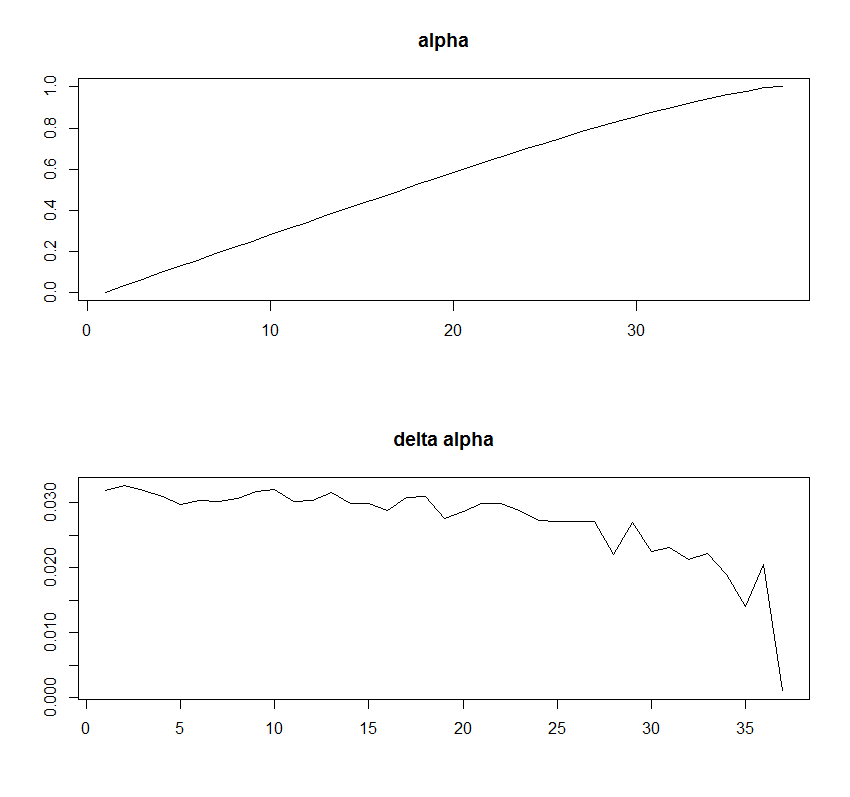
\includegraphics[width=0.6\textwidth]{figures/traj_alpha_example.png}
\end{frame}

%####################################################
\begin{frame}{Comparison with a standard Gibbs}
%####################################################

\begin{itemize}
\item 5 chains, $39\times 2000$ iterations to respect the tame  computational budget
\item Chains initialized on  $\theta^{(0)} \sim \eta_{VB}(\cdot)$
\item Convergence checked empirically
\item In the end : thining $=5$.  Sample of size $2000$. 
\end{itemize}
 
\end{frame}



%####################################################
\begin{frame}{Posterior}
%####################################################
\centering
 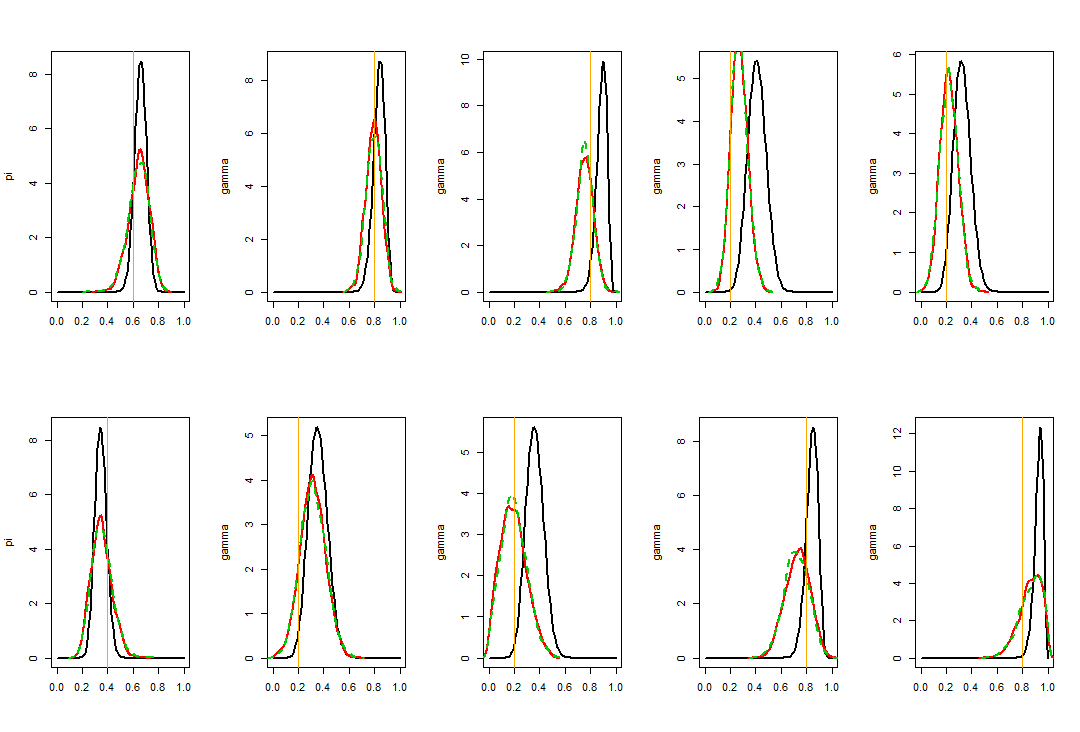
\includegraphics[width= \textwidth]{figures/post_example.png}
 
 Black : VB, Green SMC, red  MCMC
 
 See \cite{donnet2017using} for more examples
\end{frame}





 %----------------------------------------------------------------------------- 
 
 
 
\section{Conclusion}


\begin{frame}{About latent variable models}
 
 \begin{itemize}
  \item Latent variables naturally arise is many models
  \item Require specific inference methods because 
  \begin{itemize}
  \item the likelihood is not explicit anymore (NLME) 
  \item the likelihood can not be computed in a reasonnable time (SBM) 
  \item we are interested in the posterior distribution of the latent variables $p(\bZ | \bY)$ (mixture models)
 \end{itemize}
\end{itemize}

\end{frame}

  %----------------------------------------------------------------------------- 
 
 \begin{frame}{About the Bayesian inference}
  
  \begin{itemize}
  \item MCMC are VERY flexible tools to infer latent variable models
  \item Universal package for ANY model
  \item \vert However \noir
  \begin{itemize}
  \item Reach their limit for models with large latent space. 
  \item For a complicated model the MCMC will  require tunnings to make it converge, SMC may be more efficient
  \end{itemize}
  
  \item People trying to propose universal tools for other methods to get the posterior distribution (\href{https://www.r-inla.org/}{\textcolor{dgreen}{INLA}}  for gaussian latent variable models for instance...) 
  \item New tools  gathering all the possibilities :  \href{https://mc-stan.org/}{Stan}, \href{https://cran.r-project.org/web/packages/LaplacesDemon/index.html}{LaplaceDemon}...
  \end{itemize}
  
  
 \end{frame}

 



\begin{frame}[allowframebreaks=0.90]{Références}
\bibliographystyle{apalike}
 \small{\bibliography{biblio2}}
  \end{frame}
  
  
  
\end{document}

  
  \section[]{Basics in probability}




\begin{frame}\label{basics probability}
\frametitle{Random variable with a finite support}
\begin{itemize}
\item  $Z$ taking possibly a finite number of values, say $\{1, \dots,K \}$. 
\item  Distribution described by  $$\left(P(Z=k)\right)_{k=1\dots K}$$ such that $\sum_{k=1}^K P(Z=k)=1$. \vert Probability mass function \noir 
\item Or equivalently, by $\left(P(Z\leq k)\right)_{k=1\dots K}$ \vert Cumulative distribution function \noir
\item \vert Expectation\noir:  $$E[Z] = \sum_{k=1}^K k (P(Z\leq k)$$
\item \vert Example\noir: Binomial distribution : number of successes in a flip coin game over $n$ trials
\end{itemize}
\end{frame}

\begin{frame}\frametitle{Discrete random variable}
\begin{itemize}
\item  $Z$ taking possibly a infinite number of discrete values, say $\mathbb{N}$. 
\item Distribution described by $\left(P(Z=k)\right)_{k \in \mathbb{N}}$ such that $\sum_{k=1}^\infty P(Z=k)=1$. 
\item Or equivalently by $\left(P(Z\leq k)\right)_{k  \in \mathbb{N} }$
\item  \vert Expectation: \noir   $E[Z] = \sum_{k=1}^\infty k (P(Z\leq k)$
\item \vert Example\noir: Poisson distribution : $$\forall k \in \mathbb{N}, P(Z=k) = e^{-\lambda}\frac{\lambda^k}{k!}$$
\end{itemize}
\end{frame}


\begin{frame}\frametitle{Continuous random variable}
\begin{itemize}
\item $Z$ taking possibly all the values of an interval (bounded or not)  say $\Omega$. 
\item $P(Z=x)=0$ $\forall x \in \Omega$
\item \vert Density probability function \noir $f : \R \mapsto \R^{+}$ such that 
\begin{eqnarray*}
f(x) &=& 0,\quad  \forall x  \notin \Omega\\
\int_{\Omega} f(x) dx&=&1\\
P(Z\leq x )  &=& \int_{-\infty}^x f(t) dt
\end{eqnarray*}

\item $F : \R \mapsto [0,1]$, $F(t) = \int_{-\infty}^t f(x) ds$ is the \vert cumulative distribution function. \noir
\item Its expectation is $E[Z] = \int t f(t) dt$
\item \vert Examples\noir: Gaussian, exponential,uniform,  Beta distribution
\end{itemize}




\hyperlink{Introduction}{\beamerreturnbutton{Back to presentation}}

\end{frame}


\subsubsection{Hypotesis testing}
\begin{frame}[allowframebreaks]\frametitle{Bayesian Hypotesis testing}


\begin{itemize}
\item Assume that
\begin{enumerate}
\item  we know that without treatment the hallucination rate is around 0.1. 
\item  we only observe individuals under treatment
\end{enumerate}
\item One interesting hypothesis testing would be
$$ (\mathcal{H}_0): \theta < 0.1 \quad \mbox{versus} \quad   (\mathcal{H}_1): \theta >= 0.1$$ 
\end{itemize}

\begin{block}{Bayes Factor}
The Bayes factor is equal to
\begin{eqnarray*}
 B_{10}^\pi &=&\left.\frac{\P(\theta \in \Theta_1 | \bY)}{\P(\theta \in \Theta_0 | \bY)}\middle/ \frac{\P(\theta \in \Theta_1)}{\P(\theta \in \Theta_0)}\right.\\
%&=& \left. \frac{\int_{\Theta_1} \pi(\theta | \bY)d\theta }{\int_{\Theta_0} \pi(\theta | \bY)d\theta}\middle/ \frac{\P(\theta \in \Theta_1)}{\P(\theta \in \Theta_0)}\right.
\end{eqnarray*}
where $\Theta_0 = [, 0.1]$ and $\Theta_1 = [0.1, 1]$.  
\end{block}


\end{frame}

%###########################################################
\begin{frame}[allowframebreaks]\frametitle{Remarks on the Bayes factor}

\begin{itemize}
\item The Bayes Factor is a likelihood ratio
\begin{eqnarray*}
 B_{10}^\pi &=&\left.\frac{\P(\theta \in \Theta_1 | \bY)}{\P(\theta \in \Theta_0 | \bY)}\middle/ \frac{\P(\theta \in \Theta_1)}{\P(\theta \in \Theta_0)}\right.\\
&=& \left. \frac{\int_{\Theta_1} \pi(\theta | \bY)d\theta }{\int_{\Theta_0} \pi(\theta | \bY)d\theta}\middle/ \frac{\P(\theta \in \Theta_1)}{\P(\theta \in \Theta_0)}\right.\\
&=& \left. \frac{\int_{\Theta_1} \frac{\ell(\bY | \theta)\pi(\theta)}{\cancel{p(\bY)}} d\theta }{\int_{\Theta_0}  \frac{\ell(\bY | \theta)\pi(\theta)}{\cancel{p(\bY)}}d\theta}\middle/ \frac{\P(\theta \in \Theta_1)}{\P(\theta \in \Theta_0)}\right.\\
&=& \left. \frac{\int_{\Theta_1} \ell(\bY | \theta)\pi(\theta)  d\theta }{\int_{\Theta_0} \ell(\bY | \theta)\pi(\theta)d\theta}\middle/ \frac{\P(\theta \in \Theta_1)}{\P(\theta \in \Theta_0)}\right.
\end{eqnarray*}
\item In classical statistics, the likelihood is maximized (likelihood ratio test), here it is integrated over the prior distribution. 
\end{itemize}

\end{frame}

%###########################################################
\begin{frame}[fragile]\frametitle{Bayes factor in our example :  Rcode}

\begin{verbatim}
 prior_theta_0 = pbeta(0.1,1,1)
 prior_theta_1 = 1- pbeta(0.1,1,1)
 post_theta_0 = pbeta(0.1,a_post,b_post) 
 post_theta_1 = 1-pbeta(0.1,a_post,b_post)
 B10 =  1/(prior_theta_1/prior_theta_0)*
 post_theta_1/post_theta_0
 [1] 1.527133
\end{verbatim}
\end{frame}




%###########################################################



\begin{frame}\frametitle{Interpretation of Bayes factors}
 
 Jeffreys' scale {\tiny [Jeffreys (1961)]  } {\tiny [Kass and Raftery (1995)] }
 

 $$
\begin{array}{|l|c|}
   \hline
\log_{10}(B_{10}) & \mbox{Degree  of evidence in favor of Hypothesis }\\
\hline 
  \mbox{from } 0 \mbox{ to } 0.5 & \mbox{weak}     \\
 \mbox{from }  0.5 \mbox{  to }  1 &  \mbox{substantial}  \\
 \mbox{from }  1 \mbox{  to } 2   & \mbox{strong	} \\
  >2 & \mbox{Decisive}\\
   \hline
\end{array}$$


\textbf{Remarks}: 
\begin{itemize}
\item Far from being  justified on strict principles
\item $B_{10}=1/ B_{01}$: $\mathcal{H}_0$ and $\mathcal{H}_1$ are symetric.
\end{itemize}
\end{frame}


\subsubsection{Model Selection}
%%%%%%%%%%%%%%%%%%%%%%%%%%%%%%%%%%%%%%%%%%%%%%%
\begin{frame}[allowframebreaks]\frametitle{Model Selection}


\begin{itemize}
\item Assume that the observations come from two populations : one taking medecine and the other taking placebo  
\item We introduce the following notations: $\forall i=1,\dots n$: 
$$Z_i =\left\{ \begin{array}{cc} 
1 & \mbox{if  individual $i$ takes the medecine}\\
0 &  \mbox{if  individual $i$ takes the placebo}
\end{array}
\right.
$$
\item Two models in competition:  

$$(\mathcal{M}_1) \; 
Y_i \sim \mathcal{B}ern(\theta), \quad \quad (\mathcal{M}_2)\left\{ \begin{array}{cc} 
 Y_i|Z_i=0 &\sim \mathcal{B}ern(\theta_0)\\
 Y_i|Z_i=1 &\sim \mathcal{B}ern(\theta_1)
 \end{array}\right.
$$
with $\theta_0 \neq \theta_1$
\end{itemize}


\begin{block}{Question}
Which model is the most probable, given the data we observe?
\end{block}

\end{frame}

%###########################################################
\begin{frame}\frametitle{Model Selection}

\begin{itemize}
\item Model $\mathcal{M}_2$ has already been studied
\item In model $\mathcal{M}_2$ we have to unknown parameters  $(\theta_0,\theta_1)$
\item Prior on $(\theta_0,\theta_1)$ : $\pi(\theta_0,\theta_1) = \ind_{[0,1]}(\theta_0) \ind_{[0,1]}(\theta_1)$
\item Likelihood function
\begin{eqnarray*}
\ell(\bY; \theta_0, \theta_1) &=& \prod_{i=1, Z_i=0}^{n_0} \theta_0^{Y_i}(1-\theta_0)^{1-Y_i} \prod_{i=1, Z_i=1}^{n_1} \theta_1^{Y_i}(1-\theta_1)^{1-Y_i}\\
&=& \theta_0^{n_{10}}(1-\theta_0)^{n_0-n_{10}}   \theta_1^{n_{11}}(1-\theta_1)^{n_1-n_{11}}
\end{eqnarray*}
where 
\begin{itemize}
\item $n_{11}$ is the number of individuals with treatment and with hallucinations,
\item  $n_{10}$ is the number of individuals without treatment and with hallucinations,
\item  $n_1$ is the number of individuals with treatment, 
\item $n_0$ is the number of individuals without treatment. 
\end{itemize}
\item Posterior distribution : we recognize $2$ independent beta distributions
$$ \theta_1 | \bY \sim \mathcal{B}eta(n_{11}, n_1-n_{11}) \quad   \theta_0 | \bY \sim \mathcal{B}eta(n_{10}, n_0-n_{10}) $$

\end{itemize}
\end{frame}
%###########################################################

\begin{frame}\frametitle{Bayes Factor for model selection}

\begin{itemize}
\item Put a prior probability on each model $P(\mathcal M _1)$  and $P(\mathcal M _2)$ such that $P(\mathcal M _1)+ P(\mathcal M _2)=1$
\item We define Bayes factor as
$$ B_{21} = \left.\frac{\P(\mathcal{M}_2| \bY)}{\P(\mathcal{M}_1 | \bY)}\middle/ \frac{\P(\mathcal{M}_1)}{\P(\mathcal{M}_2)}\right.
$$

where
\begin{eqnarray*}
\P(\mathcal{M}_2| \bY)  =  \frac{P(\bY | \mathcal{M}_2)P(\mathcal{M}_2)}{P(\bY | \mathcal{M}_2)P(\mathcal{M}_2) + P(\bY | \mathcal{M}_1)P(\mathcal{M}_1)}
\end{eqnarray*}
\item And so : 
$$ B_{21} =  \frac{\P(\bY|\mathcal{M}_2)}{\P( \bY | \mathcal{M}_1)}  $$ 
with, in our case : 
$$ \P( \bY | \mathcal{M}_1) = \int \ell_1(\bY| \theta) \pi_1(\theta) d\theta$$ 
$$  \P( \bY | \mathcal{M}_2) = \int \ell_2(\bY| \theta_0, \theta_1) \pi_2(\theta_0,\theta_1)  d\theta_0 d\theta_1$$ 
\end{itemize}
\end{frame}
%###########################################################

\begin{frame}\frametitle{Remarks on Bayes Factor for model selection}

\begin{itemize}
\item Finally I need to be able to compute the normalizing constant (marginal likelihood) for model selection! 
\item ``Naturally'', Bayes factor will encourage the simplest models {\tiny \vert [Berger and Jefferys (1991)] \noir}
\item Automatic penalization due to the integration over the parameters 
\item Asymptotic approximation : when $n \rightarrow \infty$
Laplace development : \vert   $\Rightarrow$ \noir BIC criteria
 
 $$\log (B_{21})  \approx  \log \frac{\ell_2(\bY|\hat{\theta_2})} {\ell_1(\bY|\hat{\theta_1})} - \frac{p_2-p_1}{2}\log(n) $$ %+ K(\hat{\theta_1},\hat{\theta_2})$$

\small where $p_k$ is the number of parameters of model $\mathcal{M}_k$ and $\hat{\theta_k}$ is the maximum likelihood estimator of model $\mathcal{M}_k$. \normalsize
\item \vert But \noir  :  requires the MLE, does not take into account the prior, only in regular models, definitions of $n$ and $p$ can be difficult  when the data are not i.i.d.  \normalsize
\end{itemize}
\end{frame}


 \hyperlink{TakeHOME}{\beamergotobutton{B ack to presentation}}

  
\end{document}
% 
% 
% \section{Modèle de  mélange}
% 
% %----------------------------------------------------------------------------- 
%    \begin{frame}\frametitle{Modèle de mélange}
%    \begin{itemize}
%   \item \vert Hypothèses  \noir 
% \begin{enumerate}
% \item Les individus sont indépendants
% \item Les symptômes sont indépendants
% \item Les individus appartiennent à des groupes $g=1\dots G$ qui conditionnent leurs distributions
% \end{enumerate}
% \item On introduit 
% %$$Z_{ig} = \left\{\begin{array}{cl} 1 & \mbox{si le patient $i$ appartient au groupe  $g$} \\  0 & \mbox{sinon.} \end{array}\right.$$    
% %ou bien
%  \begin{itemize}
%   \item $$Z_{i} = \left.\begin{array}{cl} g & \mbox{si le patient $i$ appartient au groupe  $g$}  \end{array}\right.$$    
% \end{itemize}
% \item Alors \vert (modèle de mélange) \noir $\forall i=1\dots n, \forall k=1\dots K$ 
% $$\left\{ \begin{array}{cl}
% Y_{ik} | Z_i=g &\sim \mathcal{B}er(p_{kg})\\
% Z_i &\sim _{i.i.d}  \mathcal{M}_G(1; \pi_1,\dots,\pi_G)
% \end{array}
% \right.
% $$
% où $\mathcal{M}_G(1; \pi_1,\dots,\pi_G)$ est la distribution multinomiale à $G$ modalités et $1$ observation: $$\P(Z_i=g)=\pi_g, \quad \mbox{et} \quad \sum_{g=1}^G \pi_g = 1$$
%  \end{itemize}  
% \end{frame}
% %----------------------------------------------------------------------------- 
%       
% \begin{frame}\frametitle{Vraisemblance} 
% 
% \begin{itemize}
% \item \vert Paramètres: \noir$\theta = (p_{kg},\pi_g)_{k=1\dots K, g=1\dots G}$ 
% \item \vert Vraisemblance: \noir 
% \begin{itemize}
% \item $[Y_{ik}| \theta] = \sum_{g=1}^G \pi_g p_{kg}^{Y_{ik}}(1- p_{kg})^{1-Y_{ik}} $
% \item \begin{eqnarray*}
% [\bY | \theta] = \prod_{i=1}^n \prod_{k=1}^K \sum_{g=1}^G \pi_g p_{kg}^{Y_{ik}}(1- p_{kg})^{1-Y_{ik}} 
% \end{eqnarray*}
%  \end{itemize}
%  \end{itemize}
%  \end{frame}
%  %----------------------------------------------------------------------------- 
%  
% \begin{frame}{Loi  a priori}
% 
%  \begin{eqnarray*}
%  p_{kg} & \sim & \mathcal{B}eta(a_{kg},b_{kg}) \\
%  (\pi_1,\dots,\pi_G)&\sim & \mathcal{D}ir(\alpha_1,\dots,\alpha_G) \\
%  \end{eqnarray*}
%  
%  \begin{block}{où $\mathcal{D}ir$ est la loi de Dirichlet }
% \begin{itemize}
% \item Support : simplexe $\mathcal{S}_G = \left\{(\pi_1,\dots,\pi_{G-1},\pi_G)  \in [0,1] ^{G} | \sum_{g=1}^{G-1} \pi_g < 1, \pi_G = 1- \sum_{g=1}^{G-1} \pi_g\right\}$ 
% \item $[\pi_1,\dots,\pi_G] \propto \prod_{g=1}^G \pi_g^{\alpha_g-1}$ avec $\pi_G = 1 - \sum_{g=1}^{G-1} \pi_g$
% \item $E[\pi_g] = \frac{\alpha_g}{\alpha_0}$ où $\alpha_0 = \sum_{g=1}^G \alpha_g$  
% \item $Var[\pi_g] = \frac{\alpha_g(\alpha_0-\alpha_g)}{\alpha_0^2 (\alpha_0+1)}$   
% \item Uniforme: $\alpha_1= \dots= \alpha_G=1$
% \item Non informative au sens de Jeffreys: $\alpha_1= \dots= \alpha_G=1/2$
% \end{itemize}
% \end{block}
% 
% \end{frame}
% 
% %----------------------------------------------------------------------------- 
% \begin{frame}{Loi  a posteriori}
% 
% \begin{itemize}
% \item 
% 
% \begin{eqnarray*}
% [\theta | \bY] &\propto&   [\bY | \theta] [\theta]\\
% &\propto & \left[ \prod_{i=1}^n \prod_{k=1}^K \sum_{g=1}^G \pi_g p_{kg}^{Y_{ik}}(1- p_{kg})^{1-Y_{ik}}\right]  \prod_{g,k=1}^{G,K} \ind_{[0,1]}(p_{kg})  \\
% && \prod_{g=1}^G \pi_g^{\alpha_g-1}\ind_{\mathcal{S}_G}(\pi_1,\dots,\pi_G)  
% \end{eqnarray*}
% \item  Modèle non conjugué, loi a posteriori non explicite dans ce cas
% \item  \vert Moyenne a posteriori: \noir approximation  numérique de $\int \theta [\theta | \bY] d\theta$?  
% \item Approche \vert Monte Carlo \noir 
% \begin{itemize}
% \item Soit $\theta^{(1)},\dots, \theta^{(M)}$ $M$-échantillon de $[\theta | \bY]$  alors $(\theta^{(1)}\dots,\theta^{(M)})$ fournit une bonne approximation de $[\theta | \bY]$ (théorème de Glivenko-Cantelli dans $\R$)
% \item \emph{Loi des grands nombres} : $\frac{1}{M} \sum_{m=1}^M  \theta^{(m)}$ converge$^*$ vers $E[\theta | \bY]$
% \end{itemize}
% \end{itemize}
% \end{frame}
% 
% 
% %----------------------------------------------------------------------------- 
% \begin{frame}{Génération de $[\theta | \bY]$}
% 
% \begin{itemize}
% \item Génération directe impossible : on n'a pas reconnu de loi
% 
% \item On n'a pas exploité l'existence des données latentes (idée EM)
% $$\bZ = (Z_1,\dots ,Z_n) \in \{1,\dots G\}^n$$ 
% \end{itemize}
% \begin{block}{Remarque}Si on obtient un échantillon de $$(\theta^{(1)},\bZ^{(1)}), \dots, (\theta^{(M)},\bZ^{(M)}) \sim [\theta, \bZ | \bY]$$  alors \vert marginalement \noir 
% $$\theta^{(1)},\dots \theta^{(M)} \sim [\theta | \bY]$$
% \end{block}
% 
% \end{frame}
% 
% 
% 
% %----------------------------------------------------------------------------- 
% \begin{frame}\frametitle{Génération de $[\theta ,\bZ| \bY]$}
% \begin{itemize}
% \item \begin{eqnarray*}
%  [\theta, \bZ | \bY] &\propto& [\bY | \bZ, \theta] [\bZ, \theta] = [\bY | \bZ, \theta] [\bZ |  \theta] [\theta]\\
%  &\propto& \left[\prod_{i=1}^n \prod_{k=1}^K p_{k Z_i}^{Y_{ik}}(1- p_{kZ_i})^{1-Y_{ik}}\right] \left[\prod_{i=1}^n \pi_{Z_i}\right]  
%   \prod_{k=1}^K  \prod_{g=1}^G   \ind_{[0,1]}(p_{kg})  \\&& \prod_{g=1}^G \pi_g^{\alpha_g-1}\ind_{\mathcal{S}_G}(\pi_1,\dots,\pi_G)  
%  \end{eqnarray*}
% \item \vert Pas de loi connue pour $(\theta,\bZ)$
% \end{itemize}
% 
% \end{frame}
% 
% 
% %----------------------------------------------------------------------------- 
% \begin{frame}\frametitle{Lois conditionnelles  $[\theta  | \bZ, \bY]$ et $[\bZ  | \btheta, \bY]$  }
% 
%  {\scriptsize \begin{eqnarray*}
%  [\theta | \bZ,  \bY] &\propto& [\bY | \bZ, \theta] [\bZ, \theta] = [\bY | \bZ, \theta] [\bZ |  \theta] [\theta]\\
%  &\propto& \left[\prod_{i=1}^n \prod_{k=1}^K p_{k Z_i}^{Y_{ik}}(1- p_{kZ_i})^{1-Y_{ik}}\right] \left[\prod_{i=1}^n \pi_{Z_i}\right]  
%   \prod_{k=1}^K  \prod_{g=1}^G   \ind_{[0,1]}(p_{kg})  \\&& \prod_{g=1}^G \pi_g^{\alpha_g-1}\ind_{\mathcal{S}_G}(\pi_1,\dots,\pi_G)   \\
%   &\propto&   \left[ \prod_{k=1}^K\prod_{g=1}^G \prod_{i=1, Z_i=g}^n p_{kg}^{Y_{ik}}(1- p_{kg})^{1-Y_{ik}}\right] \left[\prod_{g=1}^n \prod_{i=1, Z_i=g}^n \pi_{g}\right] \\ 
% &&  \prod_{k=1}^K  \prod_{g=1}^G   \ind_{[0,1]}(p_{kg})   \prod_{g=1}^G \pi_g^{\alpha_g-1}\ind_{\mathcal{S}_G}(\pi_1,\dots,\pi_G)  \\
% &\propto&  \vert \prod_{k=1}^K \prod_{g=1}^G \underbrace{p_{kg}^{n_{kg}}(1- p_{kg})^{n_g-n_{kg}}  \ind_{[0,1]}(p_{kg})}_{\mathcal{B}(n_{kg}+1, n_g-n_{kg}+1)} \rouge  \underbrace{\prod_{g=1}^n   \pi_{g}^{n_g} \pi_g^{\alpha_g-1}\ind_{\mathcal{S}_G}(\pi_1,\dots,\pi_G)}_{\mathcal{D}(n_{1}+\alpha_1, \dots, n_G+\alpha_G)} 
%  \end{eqnarray*}
%  avec $n_g$ le nombre d'individus du groupe $g$ et $n_{kg}$ le nombre d'individus du groupe $g$ présentant le symptôme $k$. 
% }
% \end{frame}
% %----------------------------------------------------------------------------- 
% \begin{frame}\frametitle{Loi  conditionnelle   $[\theta  | \bZ, \bY]$  }
% \begin{block}{$[\theta  | \bZ, \bY]$ }
% \begin{itemize}
% \item  $$ p_{kg} | \bZ,\bY  \sim \mathcal{B}eta(n_{kg}+1, n_g-n_{kg}+1), \forall (k,g)$$
% avec $n_g = \sum_{i=1}^n \ind_{Z_i=g}$ et  $n_{kg} = \sum_{i=1}^n \ind_{Z_i=g}Y_{ik}$
% \item $$ (\pi_1,\dots, \pi_{G})| \bZ,\bY  \sim \mathcal{D}ir(n_{1}+\alpha_1, \dots, n_G+\alpha_G) $$
% \end{itemize}
% \end{block}
% \end{frame}
% %----------------------------------------------------------------------------- 
% \begin{frame}\frametitle{Loi  conditionnelle  $[\bZ | \theta, \bY]$  }
% 
% On cherche $\forall i=1,\dots, n, \forall g=1\dots G$,
% $$ \P(Z_i=g | \bY, \theta)$$ 
% 
% $\forall g=1\dots G$, 
% \begin{eqnarray*}
% \P(Z_i=g |\bY,\theta)  &=&  \P(Z_i=g |Y_i,\theta) \propto   \P(Y_i | Z_i=g, \theta) \P(Z_i=g |\theta)\\
% & \rouge \propto \noir &\left[ \prod_{k=1}^K p_{kg}^{Y_{ik}} (1-p_{kg})^{1-Y_{ik}}\right] \pi_g  := w_{ig}\\
% \P(Z_i=g |\bY,\theta)   &=& \frac{w_{ig}}{\sum_{g=1}^G w_{ig}}
% \end{eqnarray*}
% \end{frame}
% 
% 
% %----------------------------------------------------------------------------- 
% \begin{frame}\frametitle{Lois conditionnelles  $[\theta  | \bZ, \bY]$  et $[\bZ | \theta, \bY]$ }
% \begin{block}{$[\theta  | \bZ, \bY]$ }
% \begin{itemize}
% \item  $$ p_{kg} | \bZ,\bY  \sim \mathcal{B}eta(n_{kg}+1, n_g-n_{kg}+1), \forall (k,g)$$
% avec $n_g = \sum_{i=1}^n \ind_{Z_i=g}$ et  $n_{kg} = \sum_{i=1}^n \ind_{Z_i=g}Y_{ik}$
% \item $$ (\pi_1,\dots, \pi_{G})| \bZ,\bY  \sim \mathcal{D}ir(n_{1}+\alpha_1, \dots, n_G+\alpha_G) $$
% \end{itemize}
% \end{block}
% 
% 
% \begin{block}{$[\bZ | \theta, \bY]$ }
% \begin{eqnarray*}
% \P(Z_i=g |\bY,\theta)&  \propto  &\left[ \prod_{k=1}^K p_{kg}^{Y_{ik}} (1-p_{kg})^{1-Y_{ik}}\right] \pi_g  := w_{ig},  \quad   g=1,\dots ,G\\
% \P(Z_i=g |\bY,\theta)   &=& \frac{w_{ig}}{\sum_{g=1}^G w_{ig}}
% \end{eqnarray*}
% \end{block}
% 
% 
% \end{frame}
% 
% %----------------------------------------------------------------------------- 
% \begin{frame}\frametitle{Algorithme de Gibbs}
% 
% \begin{block}{}
% \begin{enumerate}
% \item[] \vert Itération 0:  \noir Initialiser $\theta^{(0)}$  et $\bZ^{(0)}$ (par un EM par exemple) 
% \item[] \vert Itération $m$ $(m=1\dots M)$: \noir  Etant données des valeurs courantes de $\bZ^{(m-1)}$, $\theta^{(m-1)}$
% \begin{itemize}
% \item Simuler $\bZ^{(m)} \sim [\bZ| \theta^{(m-1)}, \bY]$
% $\forall i=1,\dots,n$, $\forall g=1,\dots, G$
% {\scriptsize 
% \begin{eqnarray*}
% \P(Z^{(m)}_i=g |\bY,\theta^{(m-1)})&  \propto  &\left[ \prod_{k=1}^K (p^{(m-1)}_{kg})^{Y_{ik}} (1-p^{(m-1)}_{kg})^{1-Y_{ik}}\right] \pi^{(m-1)}_g \\
% && := w^{(m-1)}_{ig},\\ %\quad   g=1,\dots ,G\\
% \P(Z^{(m)}_i=g |\bY,\theta^{(m-1)})   &=& \frac{w^{(m-1)}_{ig}}{\sum_{g=1}^G w^{(m-1)}_{ig}}
% \end{eqnarray*}
% }
% \item Simuler  $\theta^{(m)} \sim [\theta | \bZ^{(m)}, \bY]$
% {\scriptsize 
% \begin{itemize}
% \item  $n^{(m)}_g = \sum_{i=1}^n \ind_{Z^{(m)}_i=g}$ et  $n^{(m)}_{kg} = \sum_{i=1}^n \ind_{Z^{(m)}_i=g}Y_{ik}$
% \item  $ p^{(m)}_{kg} | \bZ^{(m)},\bY  \sim \mathcal{B}eta(n^{(m)}_{kg}+1, n^{(m)}_g-n^{(m)}_{kg}+1), \forall (k,g)$
% \item $ (\pi^{(m)}_1,\dots, \pi^{(m)}_{G})| \bZ,\bY  \sim \mathcal{D}ir(n^{(m)}_{1}+\alpha_1, \dots, n^{(m)}_G+\alpha_G) $
% \end{itemize}}
% \end{itemize}
% \end{enumerate}
% \end{block}
% \end{frame}
% 
% %----------------------------------------------------------------------------- 
% \begin{frame}\frametitle{Propriétés de la chaîne $(\bZ^{(m)}$, $\theta^{(m)})_{m\geq 0}$}
% \begin{block}{}
%  $(\bZ^{(m)}$, $\theta^{(m)})_{m\geq 0}$ est un processus de Markov à temps discrets $(m)$, à espace d'états continu
%  \begin{itemize}
% \item $(\bZ^{(m)}$, $\theta^{(m)})$ ne dépend que de l'itération précédente (et des données $\bY$)
% \end{itemize}
% \end{block}
% 
% \begin{block}{}
% Elle admet comme loi stationnaire $[\bZ,\theta | \bY]$ 
% \begin{itemize}
% \item i.e. si $(\bZ^{(m)}$, $\theta^{(m)}) \sim [\bZ,\theta | \bY]$ $(\bZ^{(m+1)}$, alors  $\theta^{(m+1)}) \sim [\bZ,\theta | \bY]$
% \end{itemize}
% \end{block}
% 
% \begin{block}{Convergence}
% \emph{Rappel sur les chaînes de Markov}: Si la chaîne de Markov est irréductible (tous les états communiquent entre eux), récurrente (proba de retour >0), positive (existence d'une loi stationnaire)  et apériodique alors elle converge vers son unique loi stationnaire. 
% \begin{itemize}
% \item C'est le cas ici (en général vrai, sauf cas très particulier) 
% \item Pour $m$ très grand, $(\bZ^{(m)}$, $\theta^{(m)}) \sim [\bZ,\theta | \bY]$
% \end{itemize}
% \end{block}
% \end{frame}
% 
% %----------------------------------------------------------------------------- 
% %----------------------------------------------------------------------------- 
% \begin{frame}\frametitle{Algorithme de Gibbs en général}
% 
% Si on cherche à échantillonner une loi du type $g(x_1,\dots,x_p)$  telle que toutes les lois conditionnelles $g_j(x_j | x_{\{-j\}})$  sont explicites alors l'algorithme de Gibbs s'écrit : 
% \begin{block}{}
% \begin{enumerate}
% \item[] \vert Itération 0:  \noir Initialiser $x_1^{(0)} \dots, x_p^{(0)} $ 
% \item[] \vert Itération $m$ $(m=1\dots M)$: \noir  Etant données des valeurs courantes de  $x_1^{(m-1)}, \dots, x_p^{(m-1)}$, 
% \begin{itemize}
% \item Simuler $x^{(m)}_1 \sim g_1(x_1 | x_2^{(m-1)}, \dots,x_p^{(m-1)} )$
% \item Simuler $x^{(m)}_2 \sim g_2(x_2 | x_1^{(m)}, x_3^{(m-1)}\dots,x_p^{(m-1)} )$
% \item Simuler $x^{(m)}_3 \sim g_3(x_3 | x_1^{(m)},  x_2^{(m)}, x_4^{(m-1)}\dots,x_p^{(m-1)} )$
% \item $\cdots$
% \item  Simuler $x^{(m)}_p \sim g_p(x_p | x_1^{(m)}, \dots,x_{p-1}^{(m )} )$
% \end{itemize}
% \end{enumerate}
% \end{block}
% La loi stationnaire est bien la loi jointe $g(x_1,\dots,x_p)$
% \end{frame}
% %----------------------------------------------------------------------------- 
% \begin{frame}\frametitle{Remarques sur l'échantillonnage de Gibbs }
% \begin{itemize}
% \item Nécessairement multidimensionnel (quitte à introduire des composantes du vecteur simulé artificiellement, $\bZ$ ici)
% \item Ne fonctionne pas si le nombre de paramètres est variable (ici, nombre de groupe $G$ fixé)
% \item Contraignant sur les modèles (lois conditionnelles explicites)
% \end{itemize}
% \end{frame}
% %----------------------------------------------------------------------------- 
% 
% %----------------------------------------------------------------------------- 
% \begin{frame}[fragile]\frametitle{En pratique : Code R}
% \begin{block}{}
% \begin{verbatim} 
% n = length(Znum); J = ncol(p); K = length(pi)
% Z = vapply(1:K, function(k){as.numeric(Znum==k)}, rep(1,n))
% for (b in 1:B){
%      N = colSums(Z)
%      pi = rdirichlet(1, N + d.prior)
%      p = matrix(rbeta(K*J, t(Z)%*%Y + a.prior,  
%        t(Z)*(Y==0) + b.prior), K, J)    
%       tau = exp((Y%*%t(log(p)) + 
%        (1-Y)%*%t(log(1-p)) + rep(1, n)%*%log(pi))
%       tau = tau/rowSums(tau)
%       Z = t(sapply(1:n,
%        function(i){rmultinom(1, 1, tau[i, ])}))
%    }
%    \end{verbatim}
% 
% \end{block}
% \end{frame}
% 
% 
% 
% %%%Local Variables:
% %%% mode: latex
% %%% eval: (TeX-PDF-mode 1)
% %%% ispell-local-dictionary: "francais"
% %%% eval: (flyspell-mode 1)
% %%%End:
% 

